\subsection{Corrections applied to data}
We apply a series of corrections to the measured correlation functions. We implement these by means of weights that are applied for each cluster-track pair. These are described in the following sections. 


\subsubsection{Weighting for photon purity}
Following Equation~\ref{eq:FinalSubtraction}, we weight the background-region correlation \CBR~by $(1-p)/p$ and the signal-region correlation \CSR~by $1/p$. We apply this weight cluster-by-cluster. To avoid binning effects, we fit the purity with a 3--parameter error function, as shown in Figure~\ref{fig:ErrFunc_Purity}.

\begin{figure}[h]
    \centering
    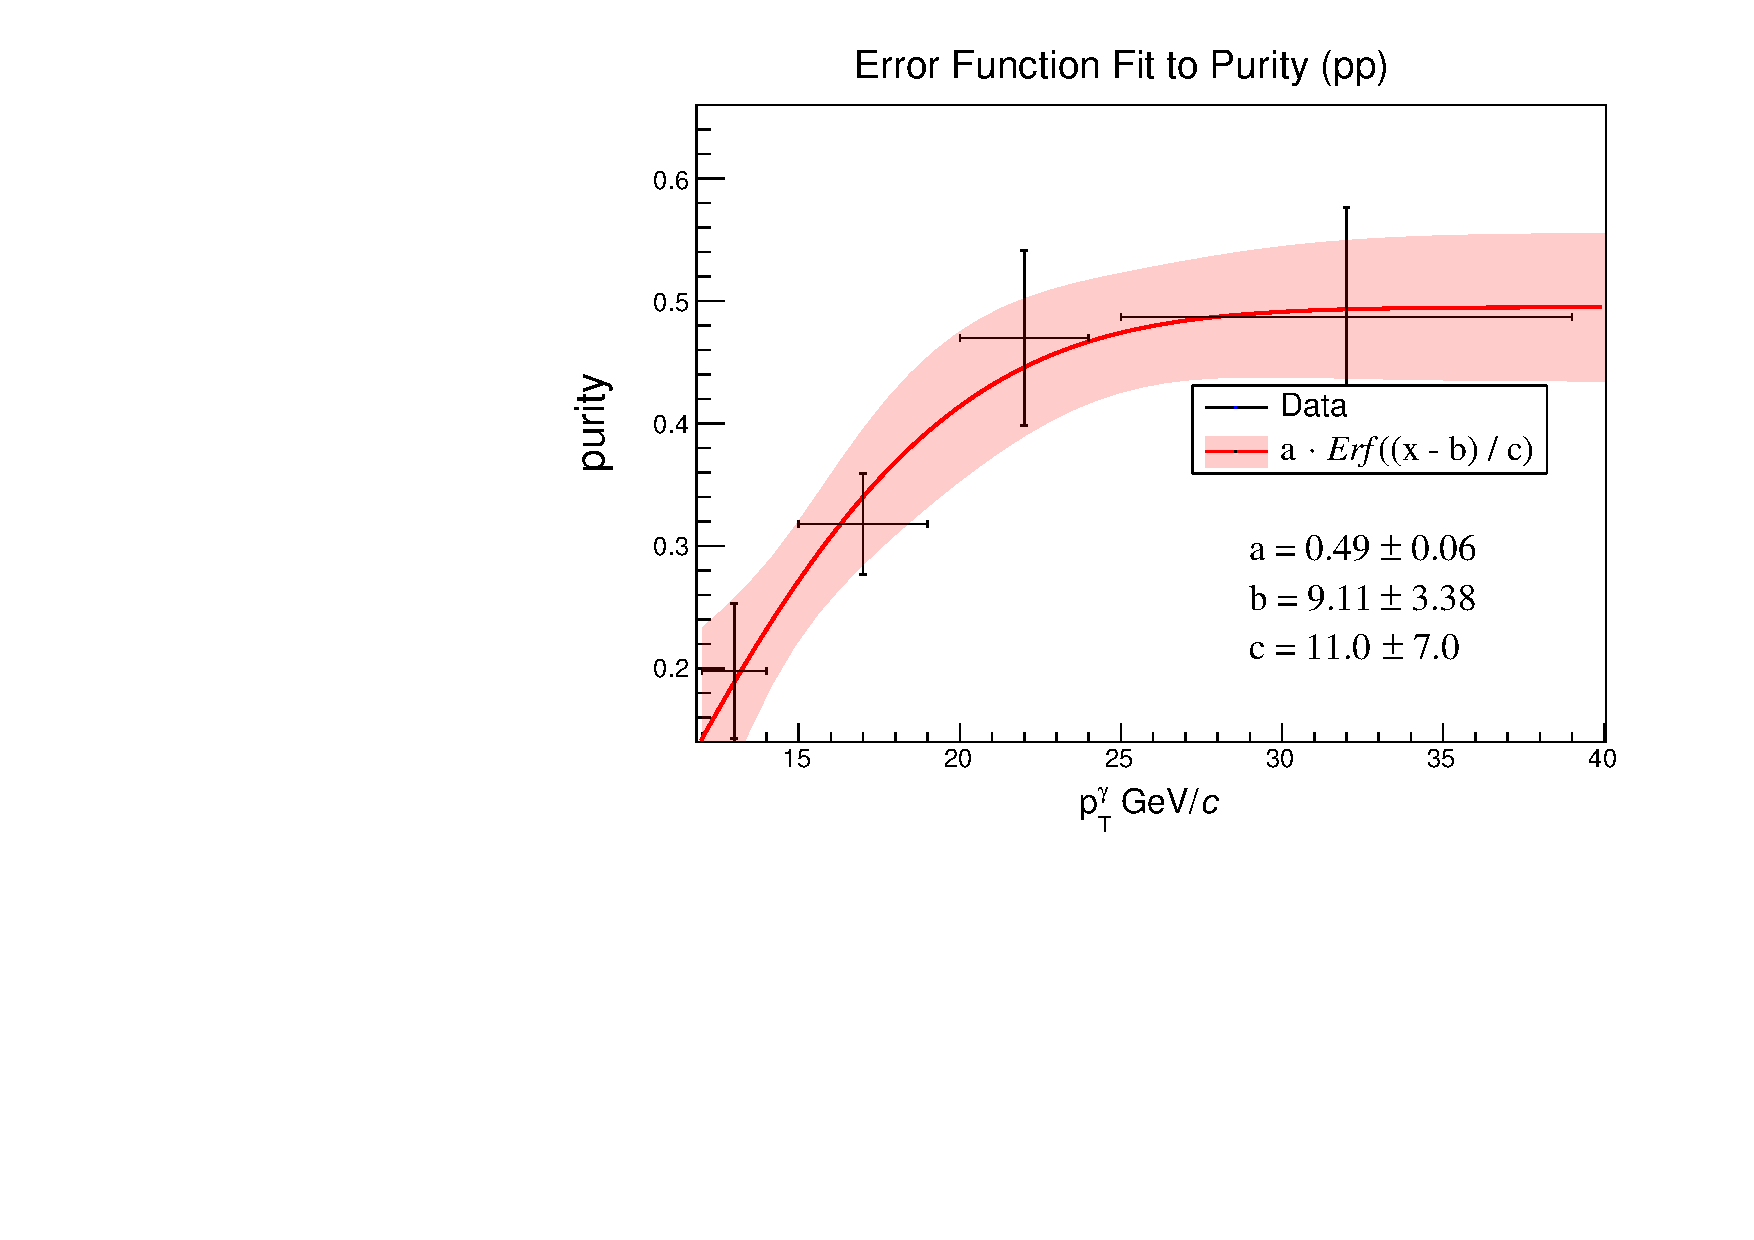
\includegraphics[width=0.49\textwidth]{G-H_New/pp_Err_Function_Purity.pdf}
    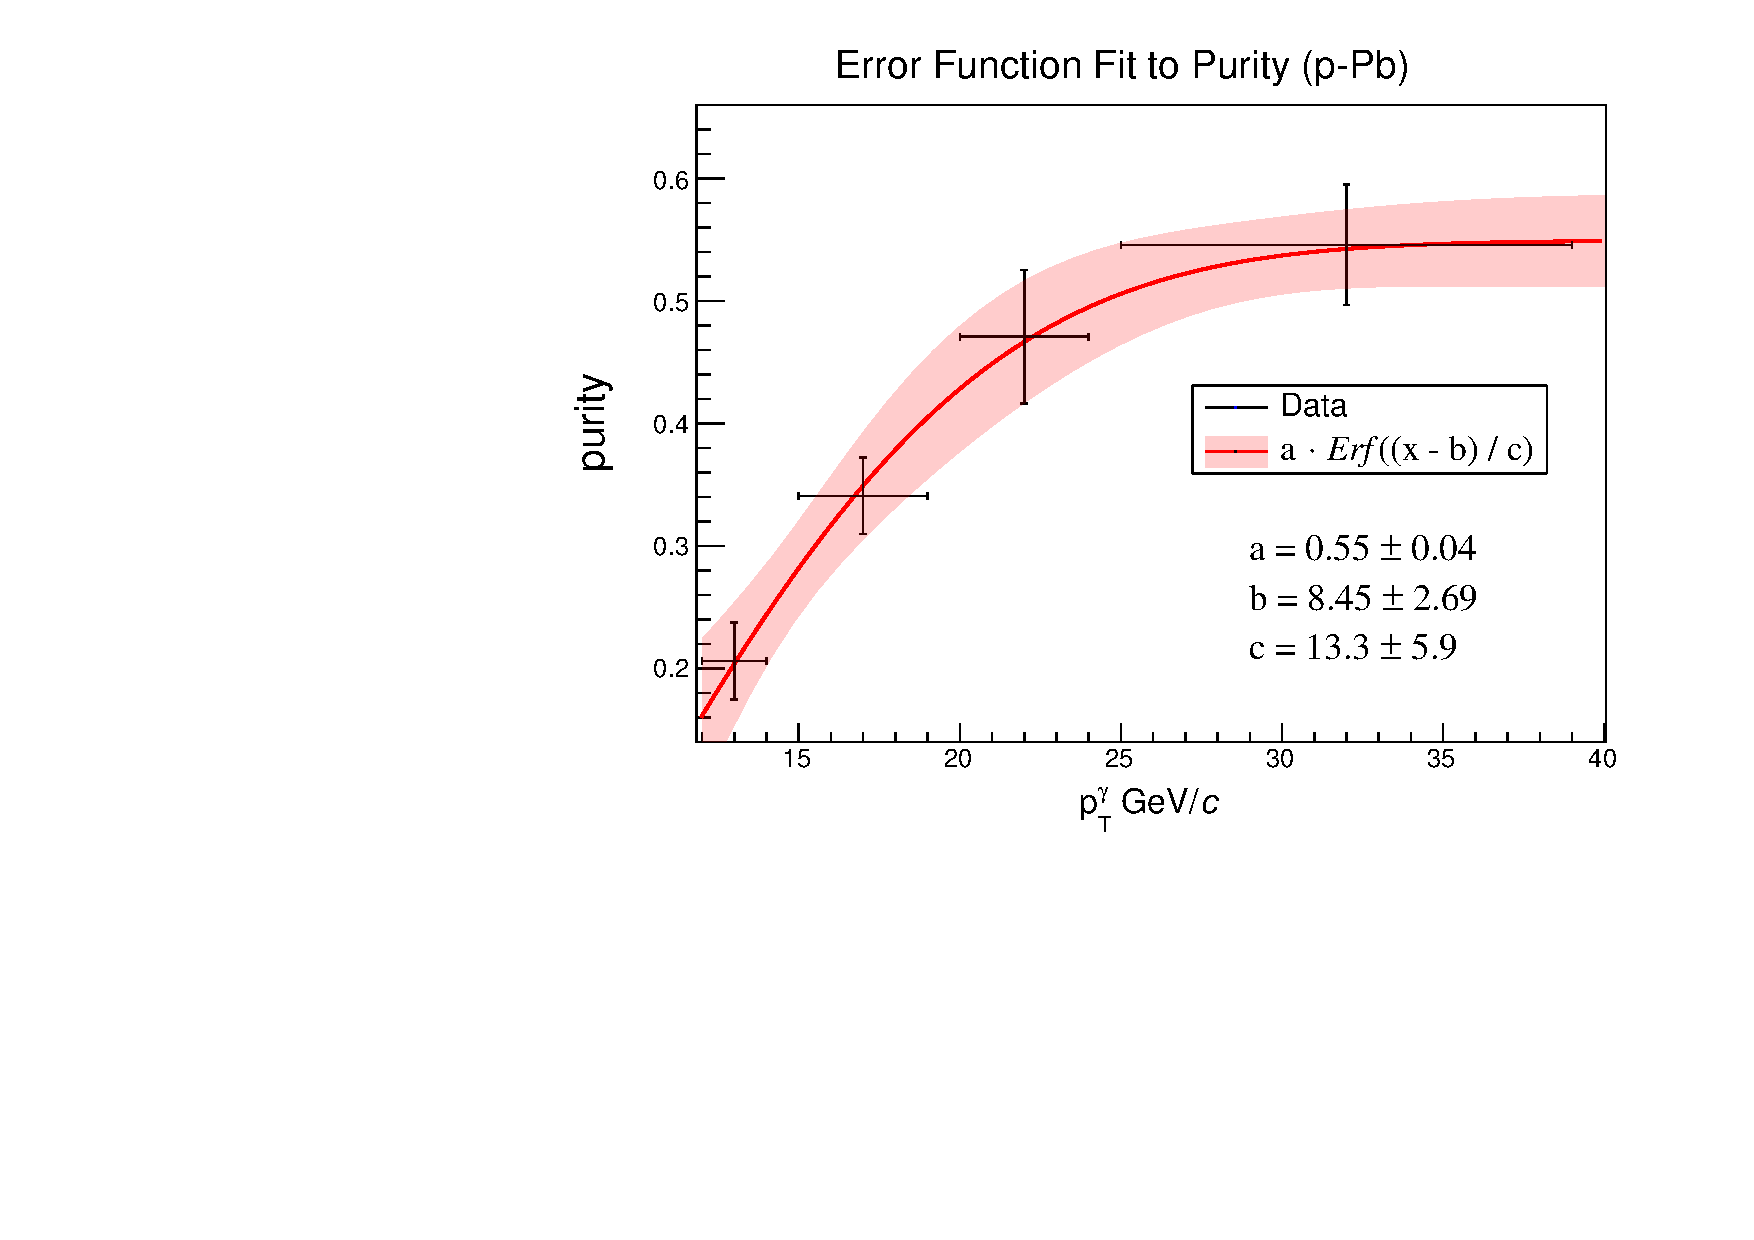
\includegraphics[width=0.49\textwidth]{G-H_New/p-Pb_Err_Function_Purity.pdf}
    \caption{A 3-parameter error function is fit to the purity values measured in pp (left) and \pPb~(right) data. The width of the band represents the uncertainty on the fit.}
    \label{fig:ErrFunc_Purity}
\end{figure}

%\subsubsection{Weighting the photon \pt~spectra of background estimate}

%The correlated background subtraction detailed in Equation~\ref{eq:FinalSubtraction} assumes that the decay-photon hadron correlation we directly measure, \CBR, is an accurate estimation of the decay-photon hadron correlation that pollutes signal region. In principle, the decay photons from neutral-meson decays that pass the shower shape cut may be biased toward pairs with a smaller opening angle (larger cluster \pt). 

%In order to correct for this effect, we weight the background-region clusters to enforce that their \pt~distribution matches that of clusters in the signal region. The cluster $\pt$ distributions before and after this weighting are shown in Figure~\ref{fig:Cluster_pT_Weight}.The effect of the weighting is negligible, because the cluster \pt~distribution in $\mathrm{SR}$ and $\mathrm{BR}$ regions are very similar. 
%\begin{figure}[h]
%    \centering
%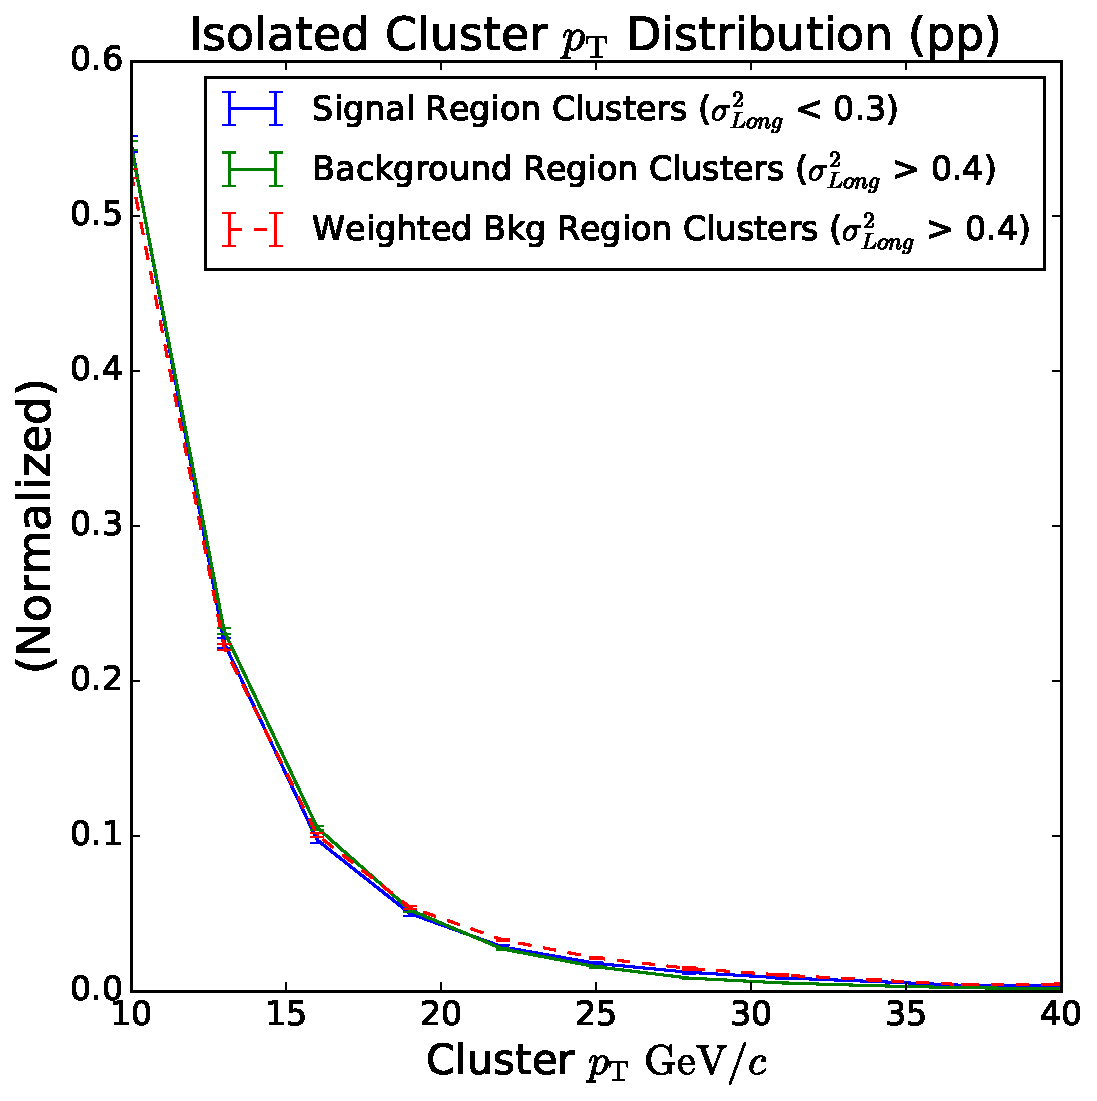
\includegraphics[width=0.49\textwidth]{G-H_New/pp_Cluster_pT_Weighted.pdf} 
%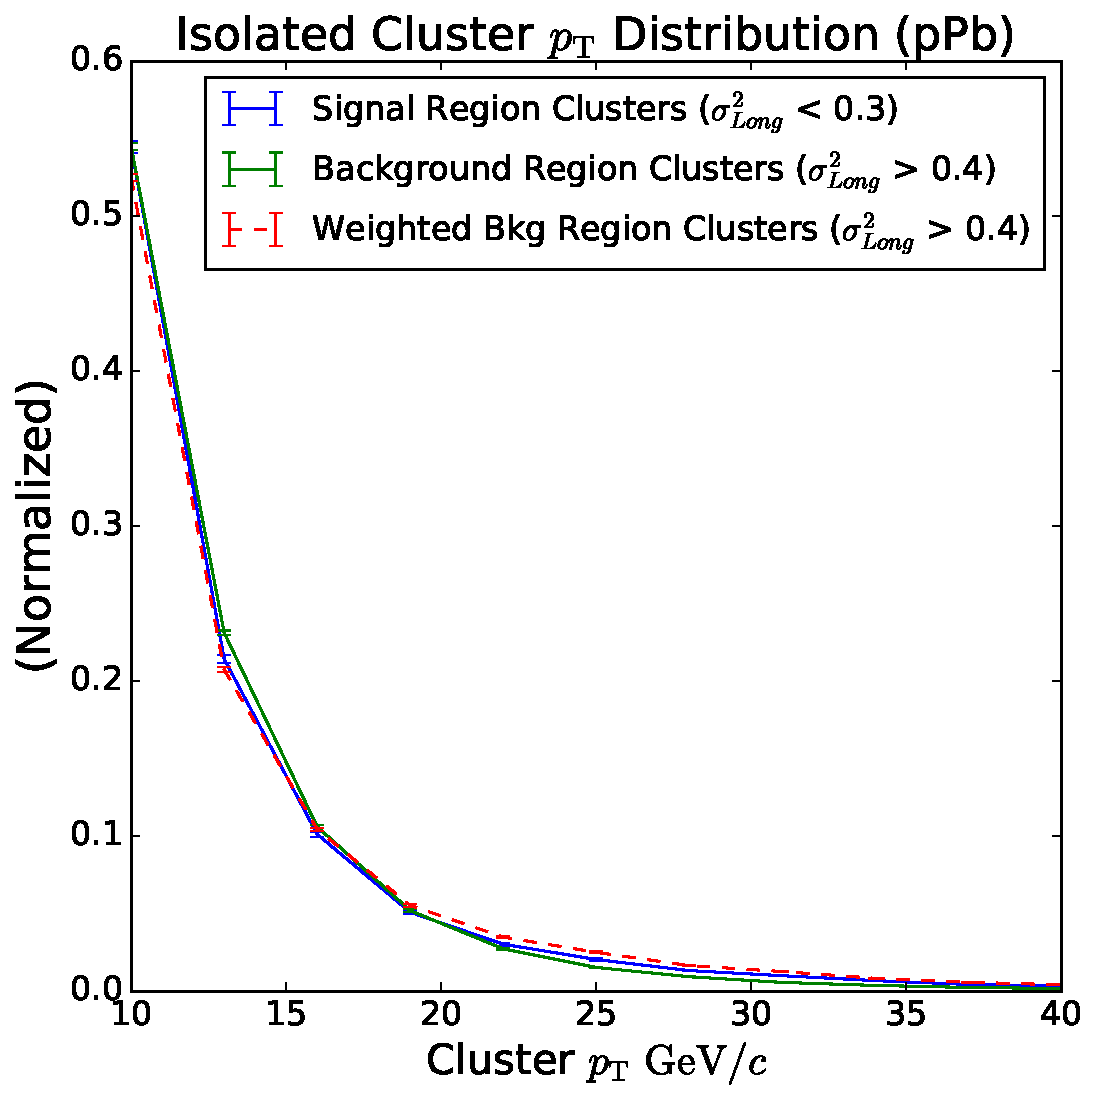
\includegraphics[width=0.49\textwidth]{G-H_New/pPb_Cluster_pT_Weighted.pdf}
    %\caption{Cluster \pt~distributions for signal and background region clusters (normalized) in pp and \pPb~collisions. }
%    \label{fig:Cluster_pT_Weight}
%\end{figure}



\subsubsection{Weighting for track efficiency, fake rate, and bin migration}
In order to correct for the tracking efficiency, fake rate, and bin-migration we apply a track-by-track weighting according to:

\begin{equation}
w_{\mathrm{tracking}}(\pt^{\mathrm{track}}) = \frac{1}{\epsilon}\times(1- f)\times b.
\end{equation}

Here $\epsilon$ is the track efficiency, $f$ is the fake rate, and $b$ is the bin-to-bin migration correction. These are described in Section~\ref{sec:tracking}. The corrections are estimated independently for pp and \pPb~data although the performance is very similar.  

\subsection{Corrected correlations}
The fully-corrected \CSR~and \CBR~correlations are shown in Figures~\ref{fig:pp_SR_BR_Overlay_pp} and \ref{fig:pPb_SR_BR_Overlay_pPb}. Our \gammaiso--hadron correlations are the difference between the scaled-\CSR~and the scaled-\CBR, which are shown in blue and red respectively. While the statistical precision of both \CSR~and \CBR~is high in all \zt~bins and datasets, this gets diluted in the subtraction. That is, the low-purity leads to the subtraction of two comparable numbers, which results in a large statistical uncertainty.

\begin{sidewaysfigure}
\centering   
    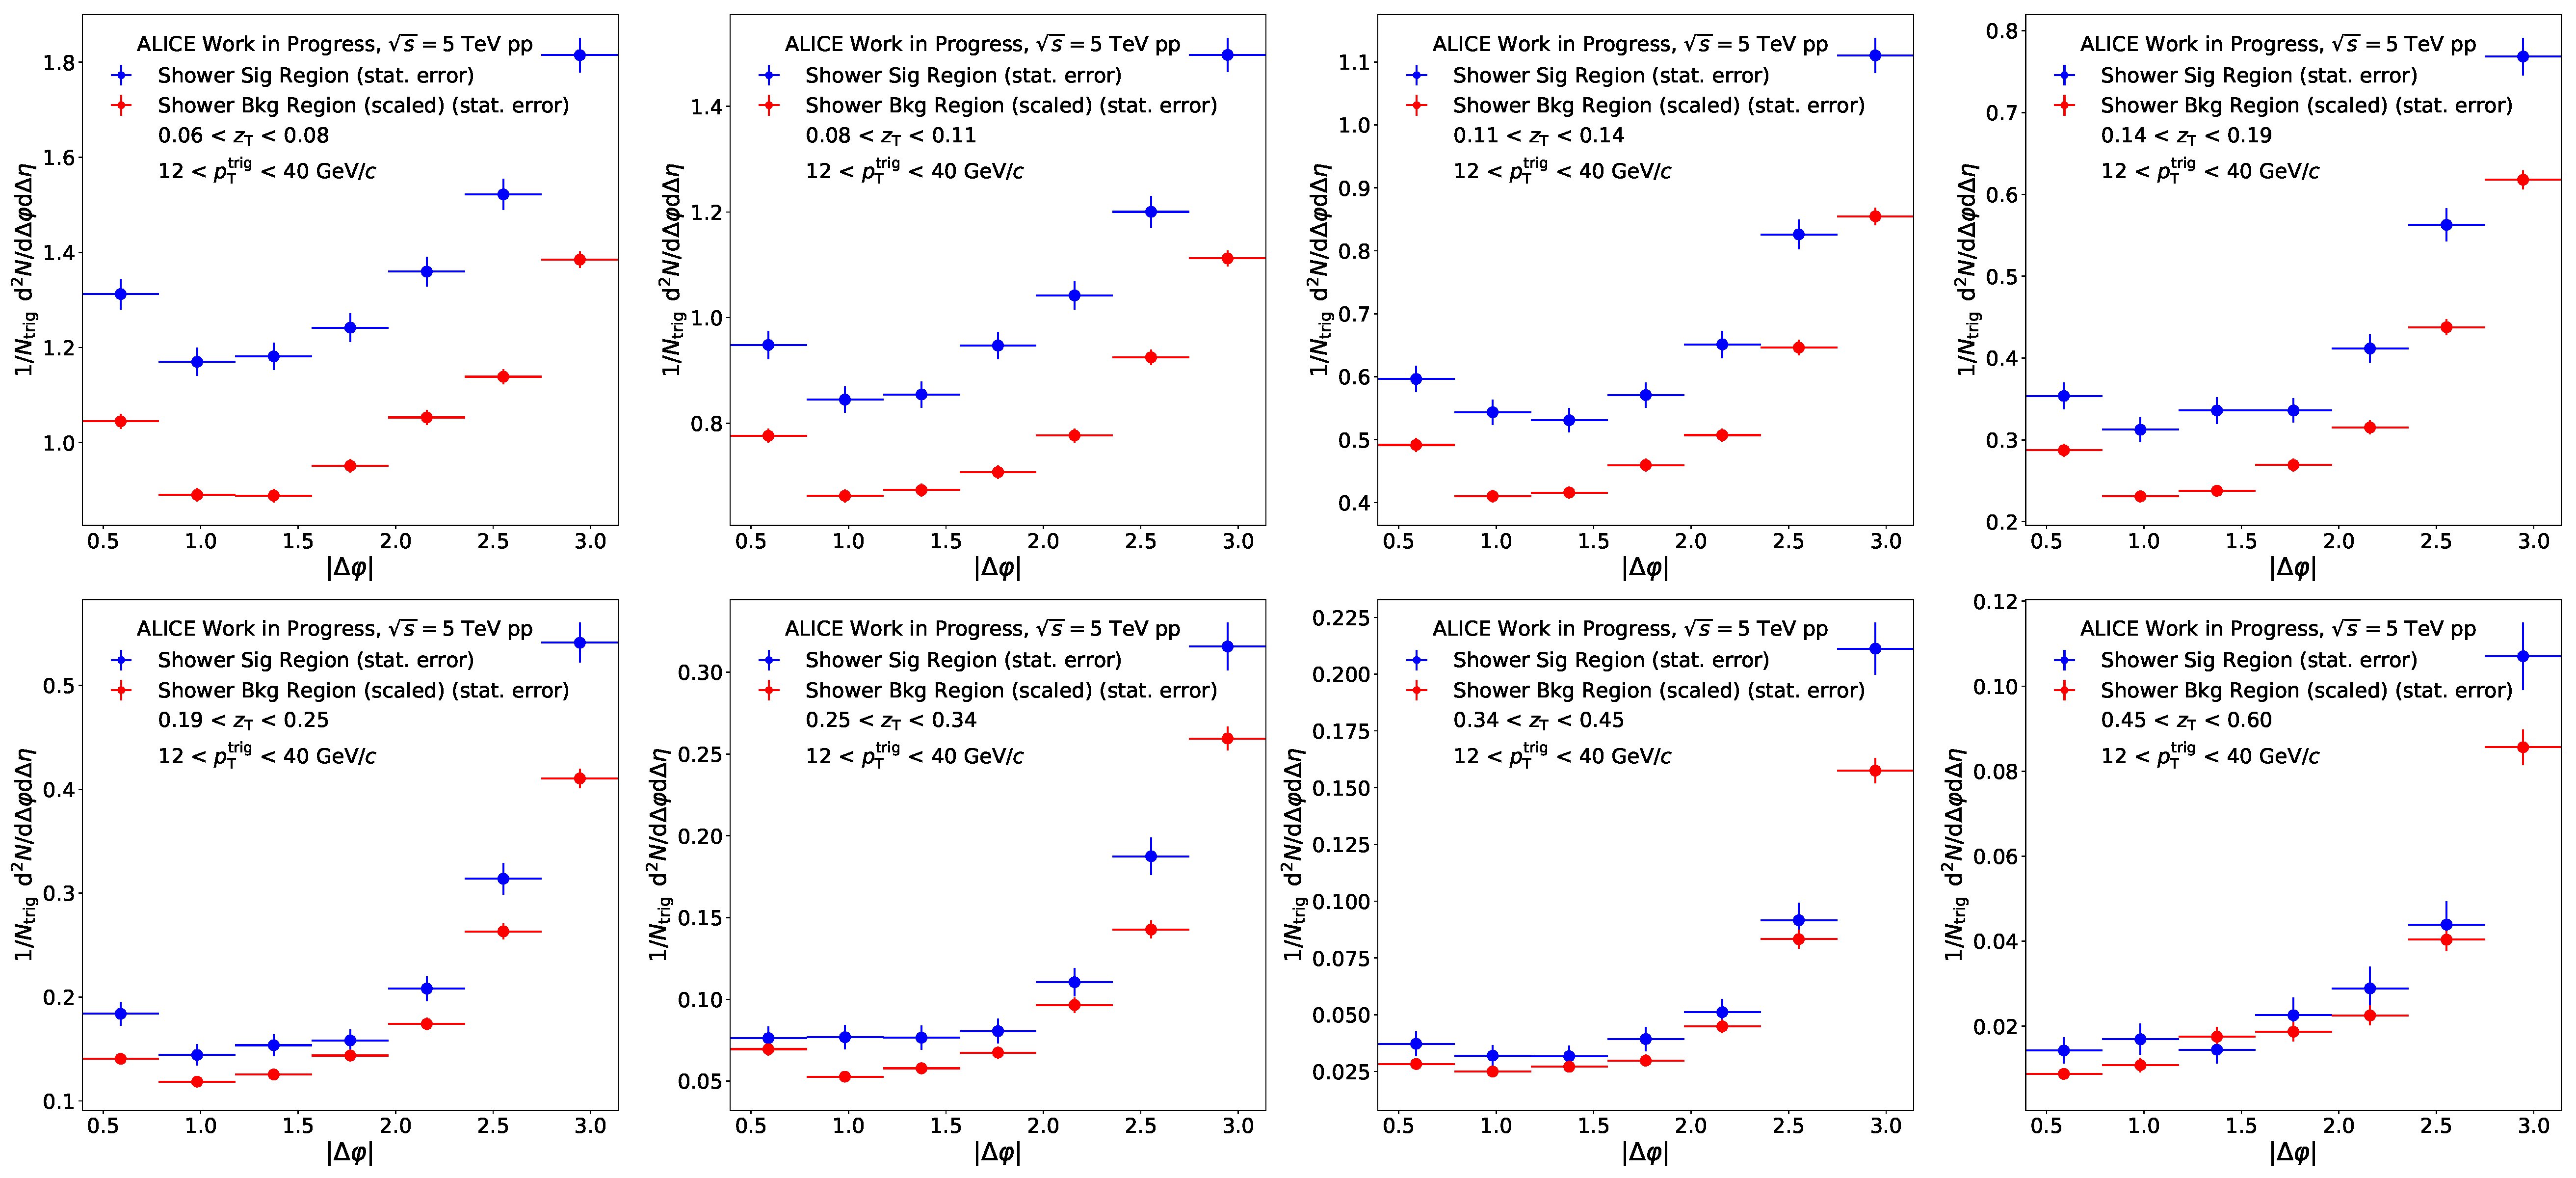
\includegraphics[width = 1.0 \textwidth]{G-H_New/pp_SR_BR_Overlay_pT_0.pdf}
    \caption{Signal-region correlation \CSR~(blue) and background-region correlation \CBR~(red) in pp collisions for various \zt~intervals. The error bars represent statistical uncertainties only.}
    \label{fig:pp_SR_BR_Overlay_pp}
\end{sidewaysfigure}

\begin{sidewaysfigure}
    \centering
    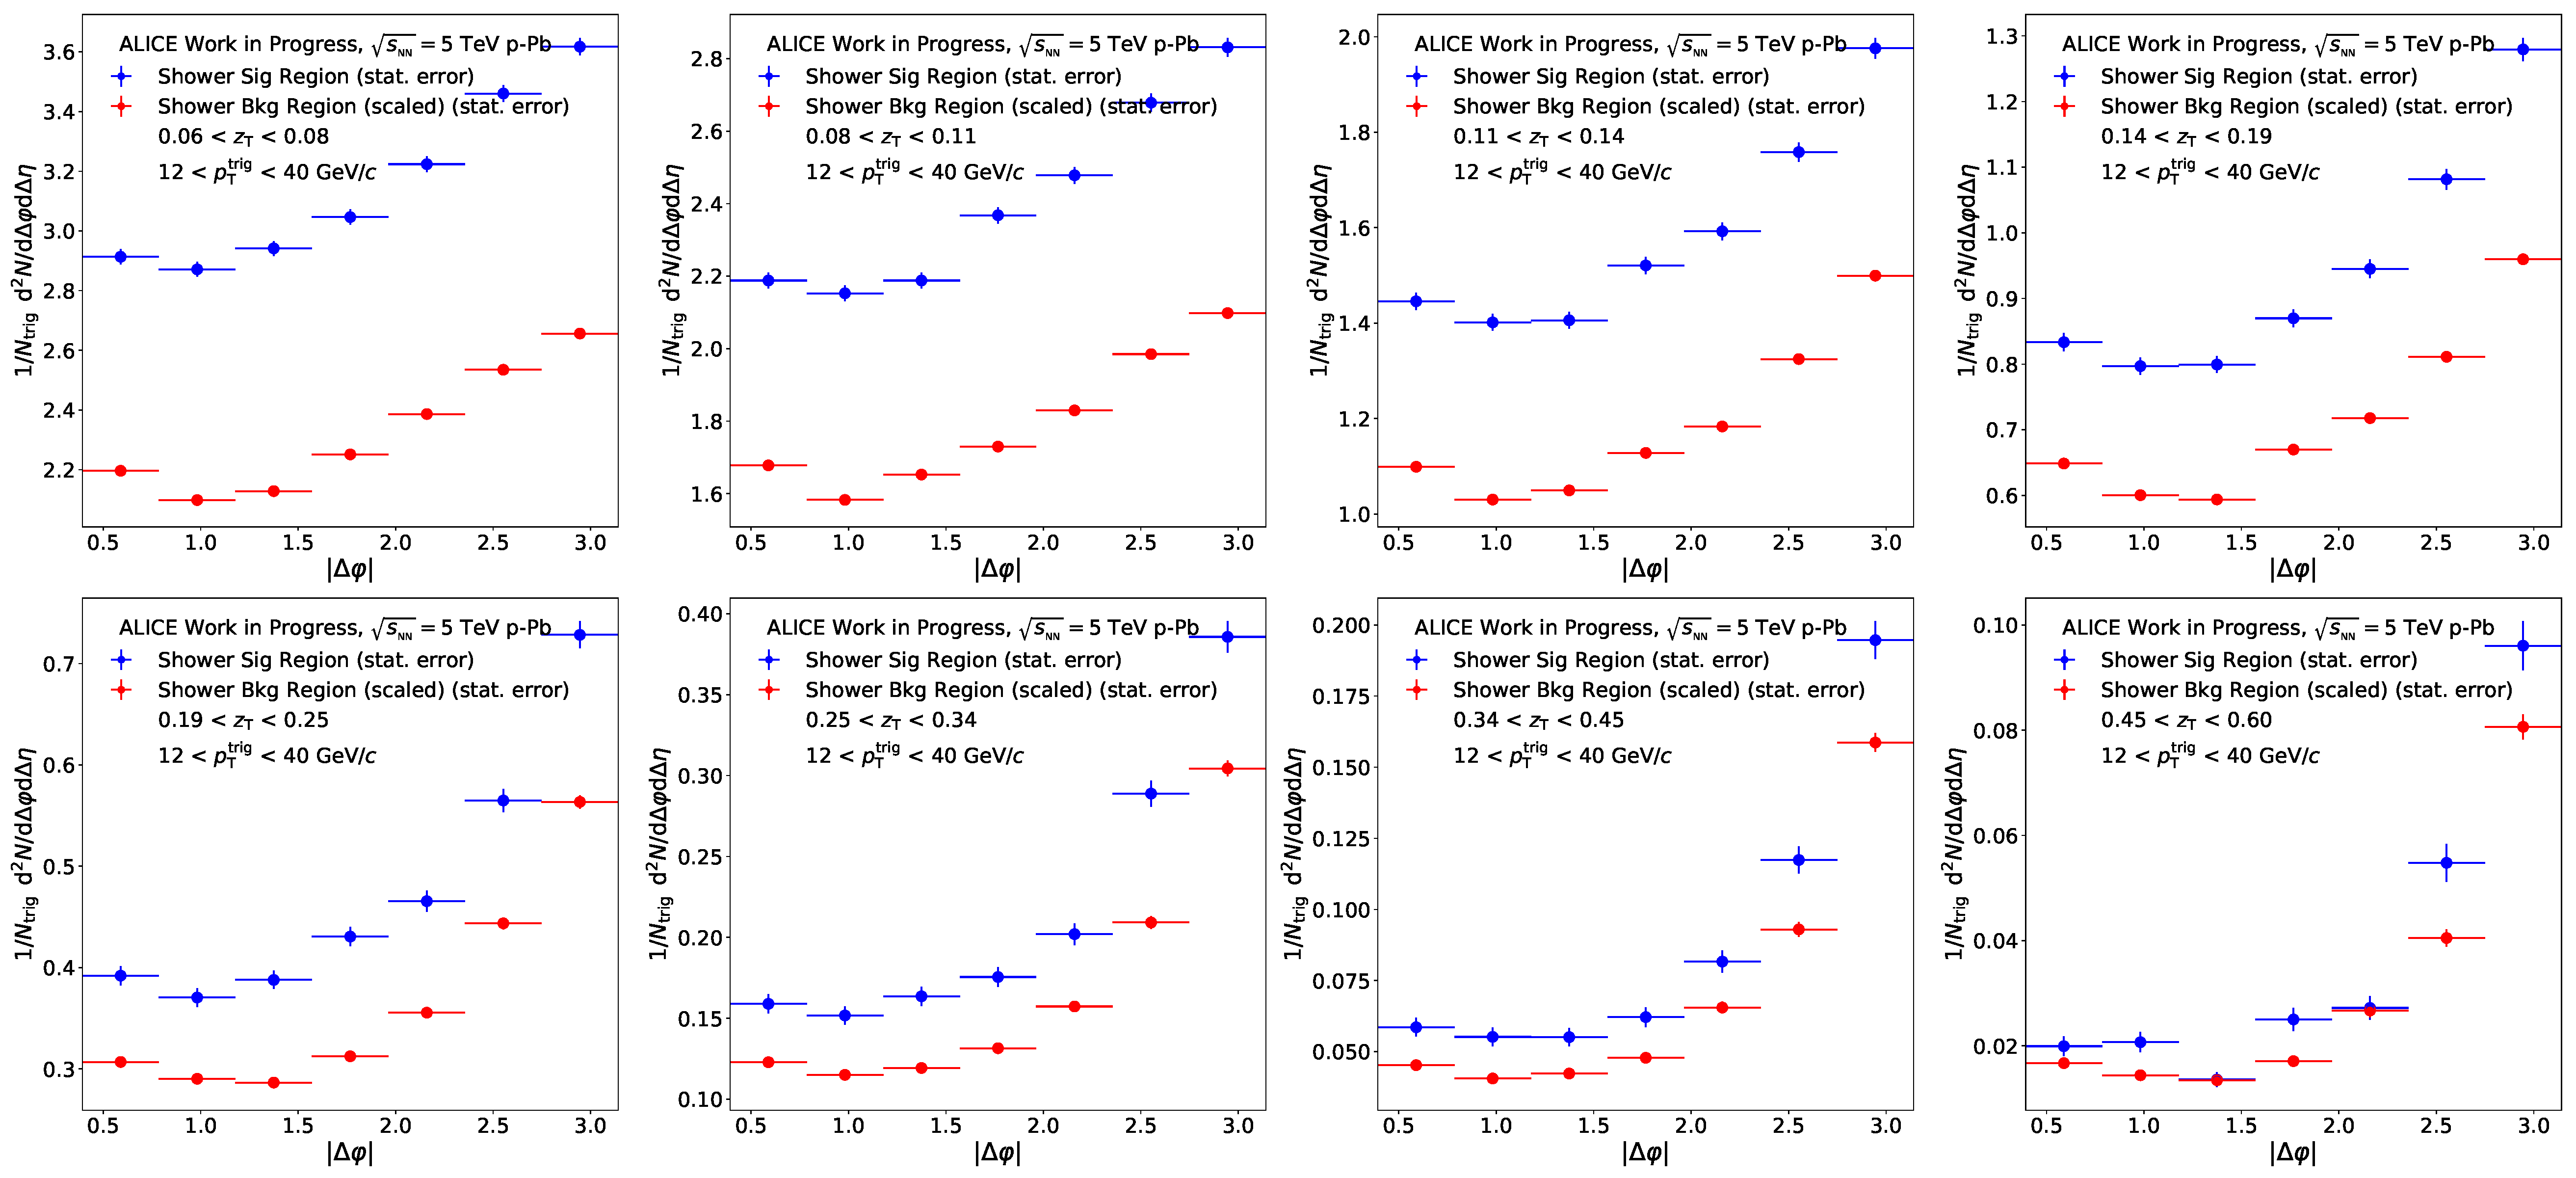
\includegraphics[width = 1.0 \textwidth]{G-H_New/p-Pb_SR_BR_Overlay_pT_0.pdf}
    \caption{Signal-region correlation \CSR~(blue) and background-region correlation \CBR~(red) in \pPb~collisions for various \zt~intervals. The error bars represent statistical uncertainties only.}
    \label{fig:pPb_SR_BR_Overlay_pPb}
\end{sidewaysfigure}
%\FloatBarrier
\subsection{Underlying event subtraction}
\label{sec:UncorrBkgnd}

This section describes the subtraction of underlying-event from the isolated photon-hadron correlations. We use a modified ZYAM procedure to estimate the uncorrelated background, where we take advantage of a feature of isolated photons-hadron correlations. The use of an isolated photon removes the near-side jet peak in the correlation function. We therefore us the $\Delta\varphi$ range of $0.4 < \Delta\varphi < 1.6$  to estimate the underlying event pedestal, and refer to this method as ZYAM moving forward.

As a check on the ZYAM procedure, we use the fact that the UE-estimation is independent of $\Delta\eta$ and that that genuine correlations due to hard-scatterings decrease as $\Delta\eta$ increases. To this end, we pick a region that is dominated by UE and extrapolate back to the region that would normally contains both UE and hard-scattering contribution. The UE is estimated by projecting the large $\Delta\eta$ region defined as $0.8 < |\Delta\eta| < 1.4$ onto the $\Delta\varphi$ axis. To minimize bias from the isolation cut as well as the away side jet peak, the uncorrelated background is estimated from the projection in the region $0.4 < \Delta\varphi < 1.4$. This $\Delta\varphi\Delta\eta$ region is illustrated in Figure~\ref{fig:LE_Map}. 

The statistical uncertainty in the UE estimate method is taken as a systematic uncertainty for $\Delta\varphi$ correlations as it is completely correlated bin-to-bin in $\Delta\varphi$.

\begin{figure}[h]
\center
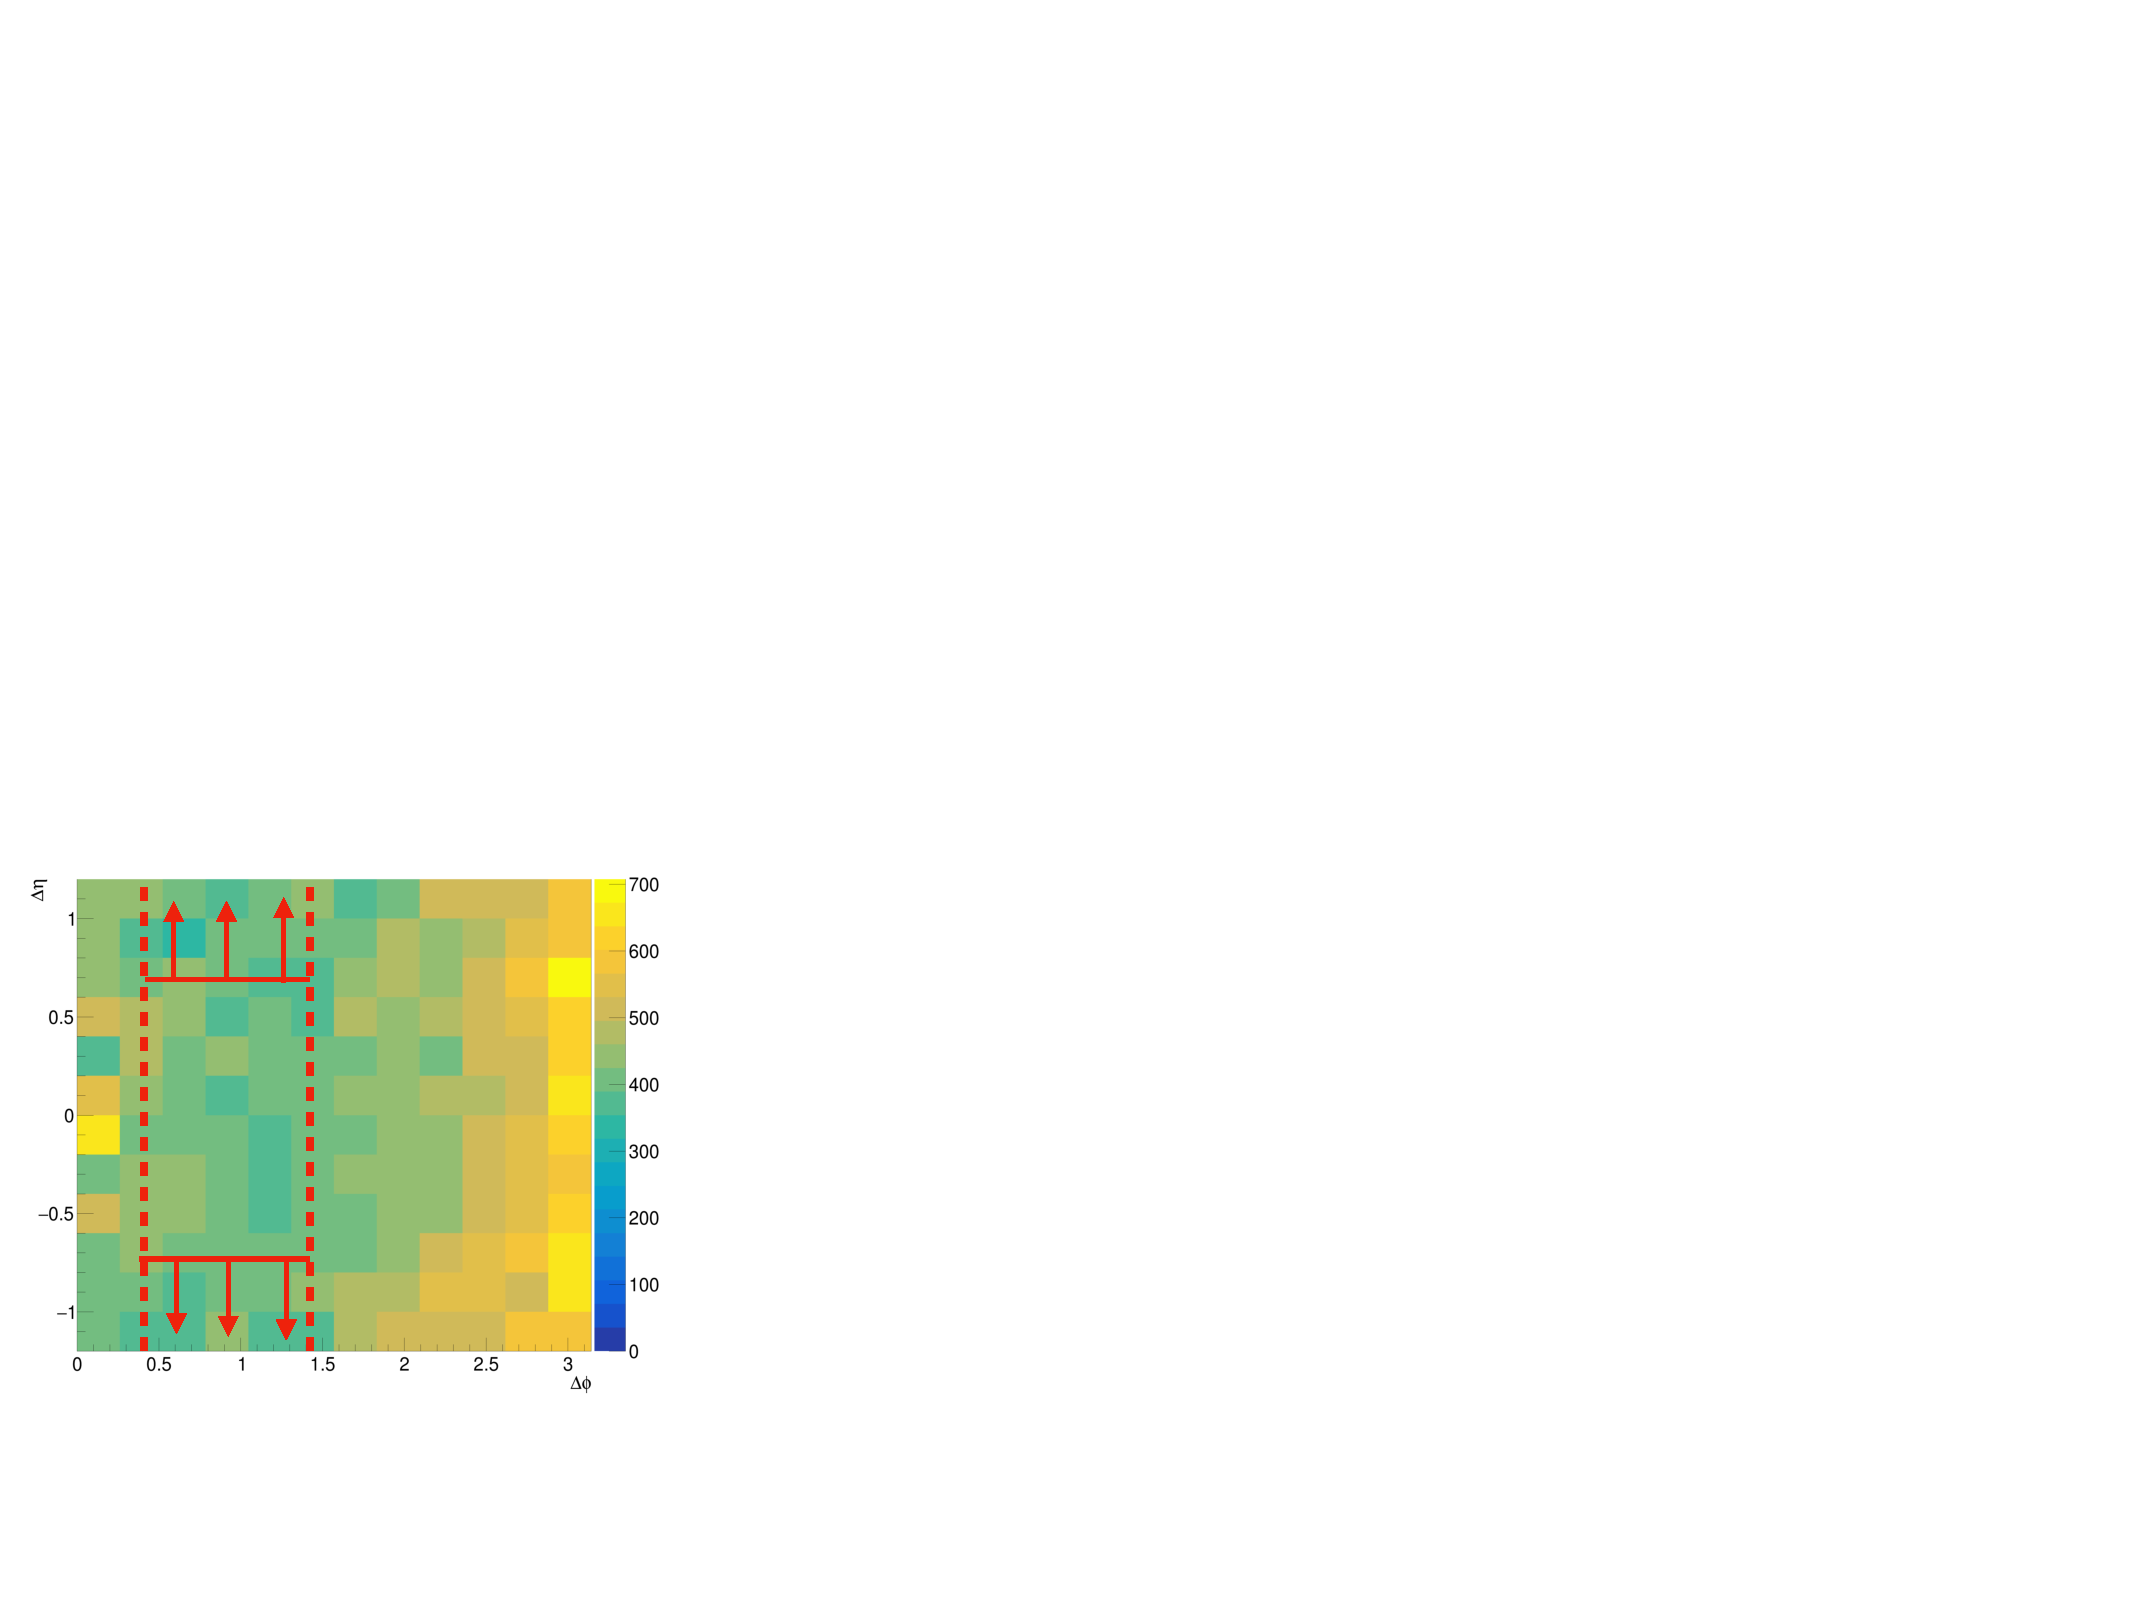
\includegraphics[width=0.5\textwidth]{EventMixing/LE_map.pdf}
\caption{The 2D region used to calculate the uncorrelated background. The $\Delta\varphi$ region is chosen to avoid the away side jet peak, as well as our isolation region of R$=$0.4. The $\Delta\eta$ region is chosen assuming that genuine correlations from hard-scatterings decrease as $\Delta\eta$ increases. The large $\Delta\eta$ is projected onto the $\Delta\varphi$ axis, and then averaged within region of 0.4 $<\Delta\varphi<$ 1.4. ZYAM is estimated in the region $ 0.4 < \Delta\varphi < 1.4$, but for our full $\Delta\eta$ range ($-1.2 < \Delta\eta < 1.2$).}
\label{fig:LE_Map}
\end{figure}

Figure~\ref{small_uncorr} shows the two UE estimates compared with the isolated photon-hadron $\Delta\varphi$ 
%bvj projections 
correlations for only 2 \zt~bins in order to show detail. The full detail of our two UE estimates is shown in Tables~\ref{tab:UE_Average} for pp and \pPb~data. The two estimates are consistent within uncertainties for almost all \zt~bins in both pp and \pPb~data. For the only case where a significant disagreement is observed, which is for the lowest \zt~bin in \pPb~data, we add in quadrature the difference as an additional systematic uncertainty. 

\begin{figure}[h]
	\center
	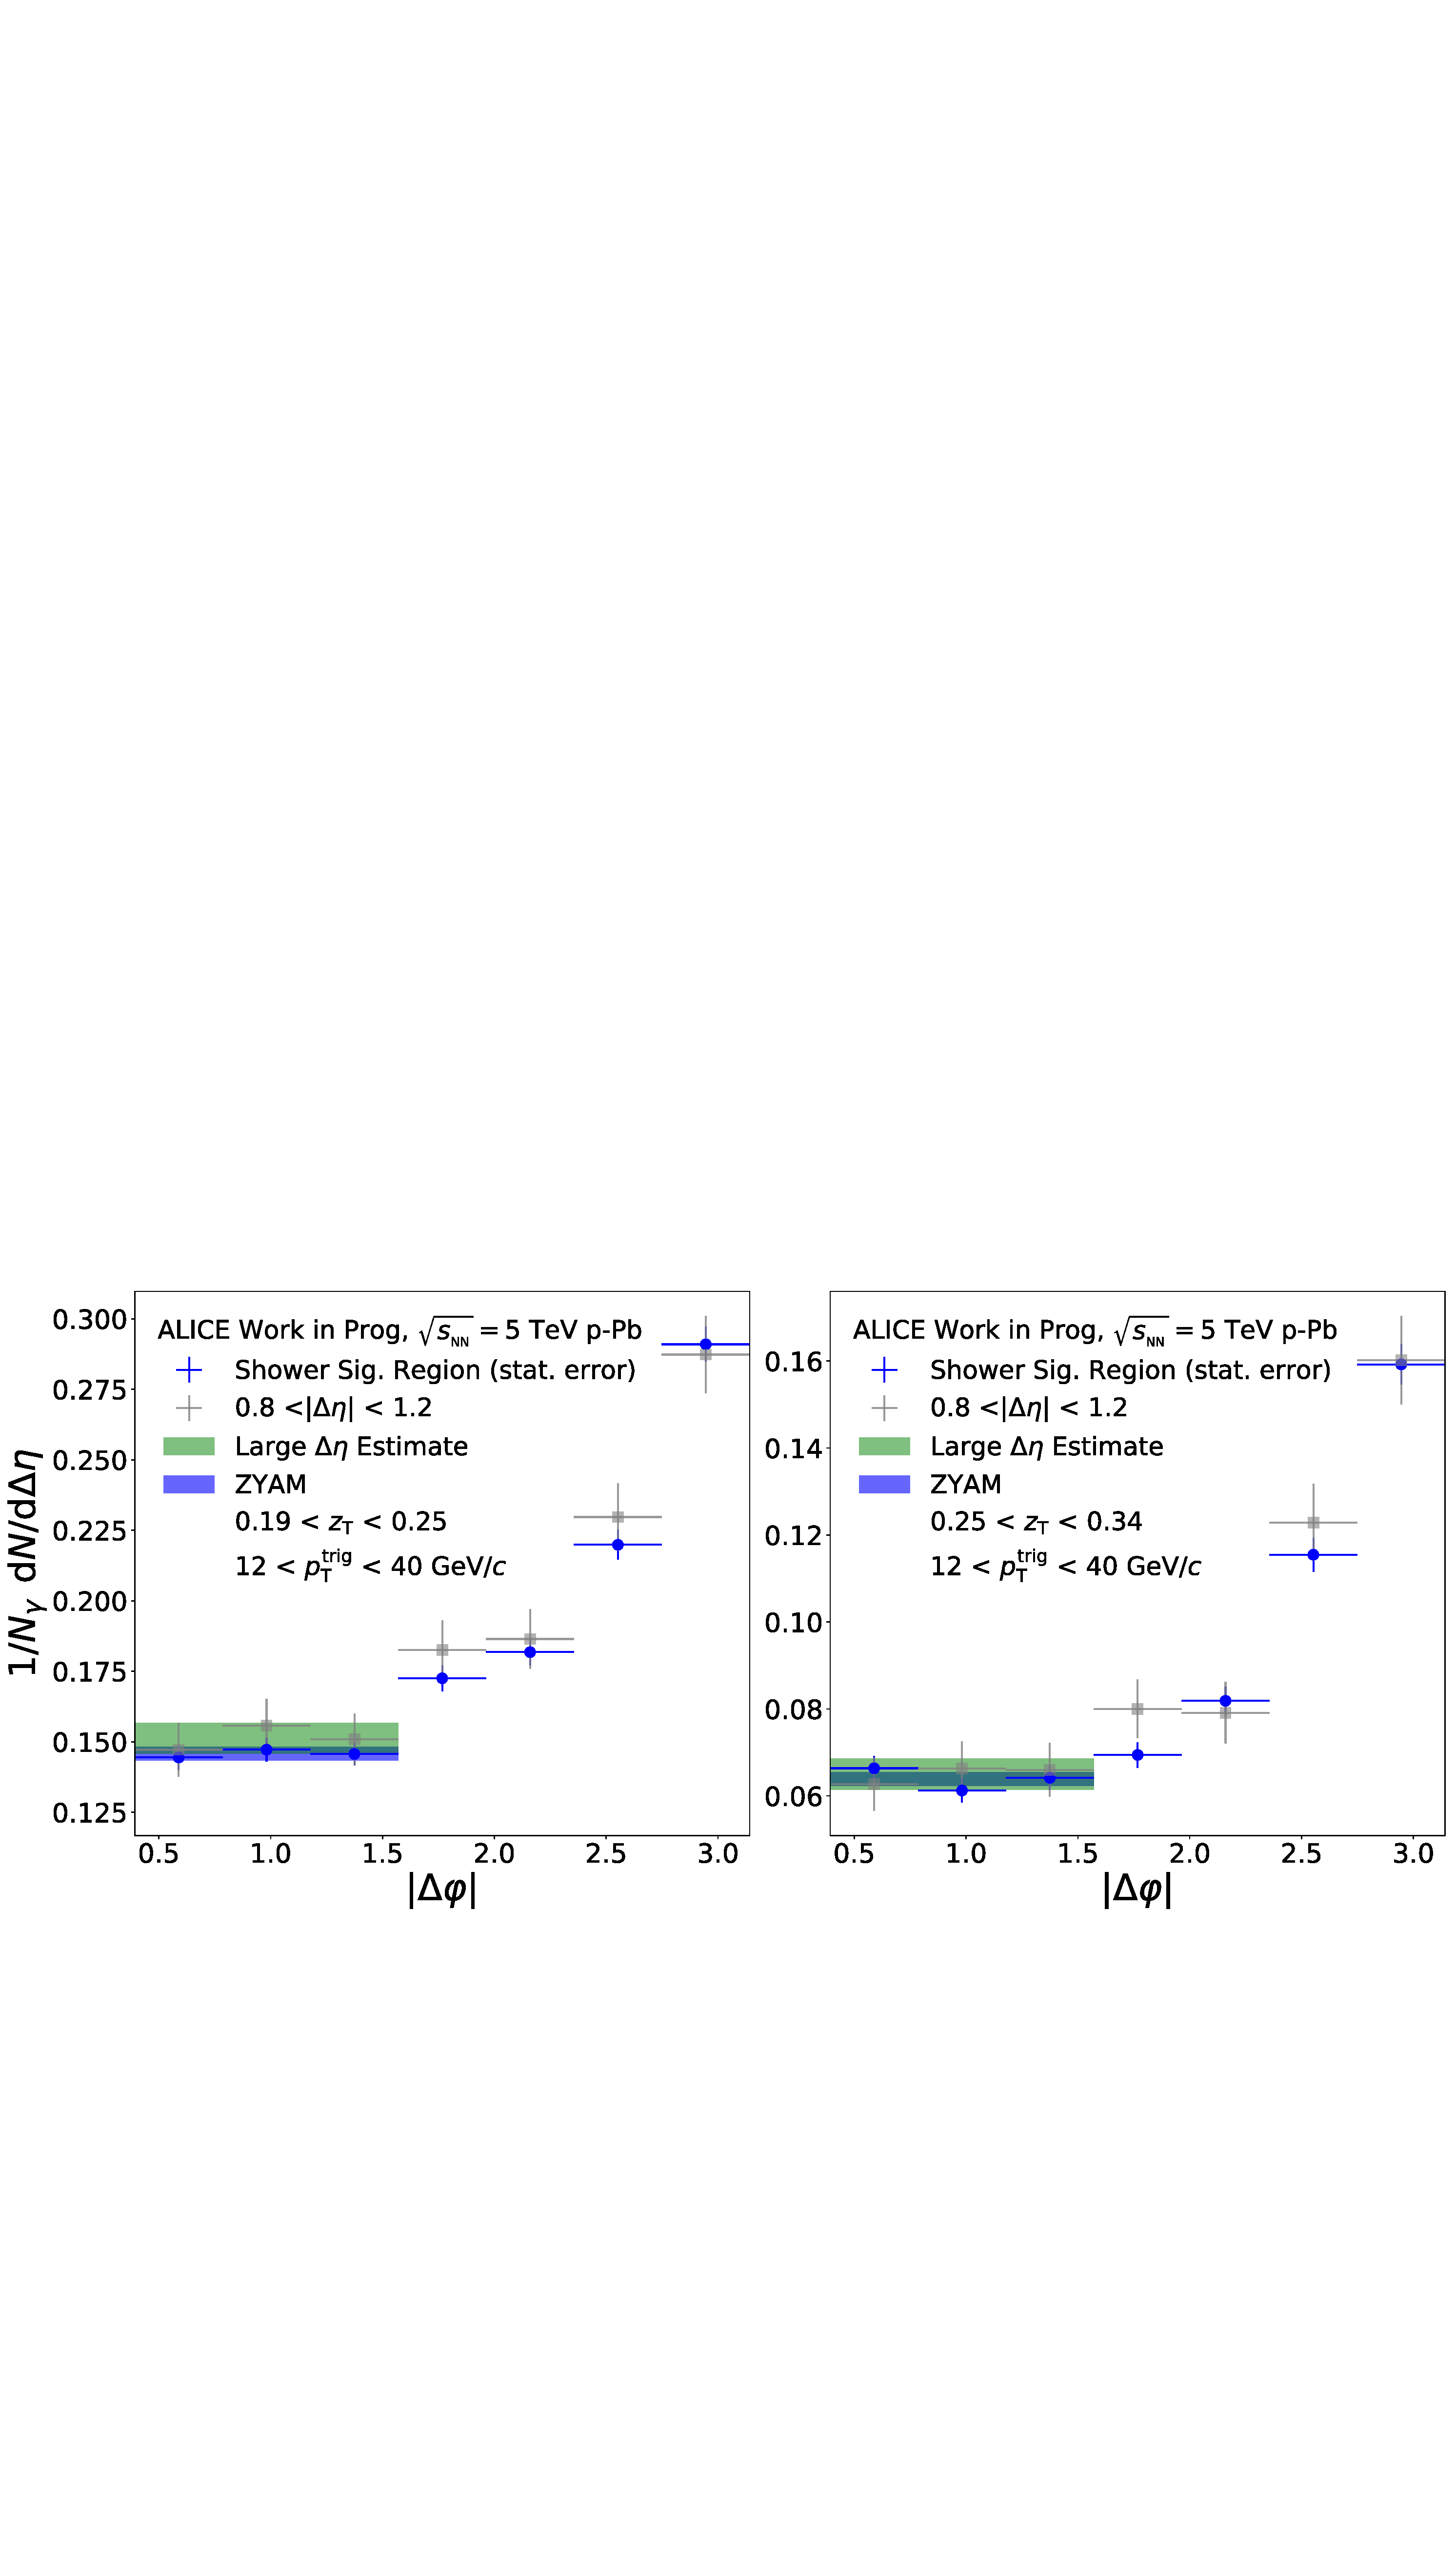
\includegraphics[width=.99\textwidth]{G-H_New/UE_Plot_p-Pb_Single.pdf}
\caption{Projections of the $\gammaiso$--hadron correlations in \pPb~collisions in 2 $\zt$~bins after correlated subtraction with UE estimates plotted. The grey points represent the large $\Delta\eta$ region ( $ 0.8 < |\Delta\eta| < 1.2$) projected onto the $\Delta\varphi$ axis. The blue band represents the region used to calculate ZYAM and the green band represents the region of large $\Delta\eta$ points used to calculate the Large $\Delta\eta$ estimate.}
\label{small_uncorr}
\end{figure}


\begin{table}
   \centering
      \caption{Summary of UE-pedestal estimates with ZYAM and the $\Delta\eta$ method for various $\zt$ bins, as well as the difference between LE and ZYAM estimates. The background estimate is shown in units of pairs per trigger. The uncertainty quoted is statistical only.}
   \begin{tabular*}{1.0\columnwidth}{@{\extracolsep{\fill}}lccc@{}}
    \hline
		$z_\mathrm{T}$ interval & ZYAM  & Large $\Delta\eta$ & Difference\\
		\hline
		pp & & \\
		\hline
0.06 - 0.08 & 0.480 $\pm$ 0.007 & 0.472 $\pm$ 0.015 & 0.008 $\pm$ 0.016\\
0.08 - 0.11 & 0.347 $\pm$ 0.006 & 0.346 $\pm$ 0.012 & 0.000 $\pm$ 0.014\\
0.11 - 0.14 & 0.219 $\pm$ 0.005 & 0.209 $\pm$ 0.010 & 0.009 $\pm$ 0.011\\
0.14 - 0.19 & 0.131 $\pm$ 0.004 & 0.129 $\pm$ 0.008 & 0.002 $\pm$ 0.008\\
0.19 - 0.25 & 0.063 $\pm$ 0.002 & 0.058 $\pm$ 0.005 & 0.005 $\pm$ 0.006\\
0.25 - 0.34 & 0.030 $\pm$ 0.002 & 0.025 $\pm$ 0.003 & 0.005 $\pm$ 0.004\\
0.34 - 0.45 & 0.013 $\pm$ 0.001 & 0.015 $\pm$ 0.003 & 0.002 $\pm$ 0.003\\
0.45 - 0.60 & 0.006 $\pm$ 0.001 & 0.005 $\pm$ 0.002 & 0.001 $\pm$ 0.002\\
	\hline 
	\pPb & & \\
	\hline
0.06 - 0.08 & 1.142 $\pm$ 0.006 & 1.190 $\pm$ 0.013 & 0.047 $\pm$ 0.014\\
0.08 - 0.11 & 0.855 $\pm$ 0.005 & 0.864 $\pm$ 0.011 & 0.010 $\pm$ 0.012\\
0.11 - 0.14 & 0.557 $\pm$ 0.004 & 0.566 $\pm$ 0.009 & 0.009 $\pm$ 0.010\\
0.14 - 0.19 & 0.318 $\pm$ 0.003 & 0.317 $\pm$ 0.007 & 0.001 $\pm$ 0.007\\
0.19 - 0.25 & 0.151 $\pm$ 0.002 & 0.159 $\pm$ 0.005 & 0.009 $\pm$ 0.005\\
0.25 - 0.34 & 0.062 $\pm$ 0.001 & 0.062 $\pm$ 0.003 & 0.000 $\pm$ 0.003\\
0.34 - 0.45 & 0.022 $\pm$ 0.001 & 0.021 $\pm$ 0.002 & 0.001 $\pm$ 0.002\\
0.45 - 0.60 & 0.007 $\pm$ 0.000 & 0.006 $\pm$ 0.001 & 0.001 $\pm$ 0.001\\

   \end{tabular*}
   \label{tab:UE_Average}
\end{table}

In order to show the effect of pedestal subtraction on the correlation functions in pp and \pPb~data, we overlay the correlation functions in both systems in Figure~\ref{fig:BF_UE_zT_second} . By construction, the points at small $\Delta\varphi$ are consistent with zero as demonstrated by the dark grey bands. Additionally, the figures demonstrate the larger underlying event in \pPb~data, as well as the agreement in away side yields in the two systems after pedestal subtraction. This also shows visually the fraction of signal to background, particularly at low \zt~in \pPb~collisions.


\begin{sidewaysfigure}[ht]
\centering
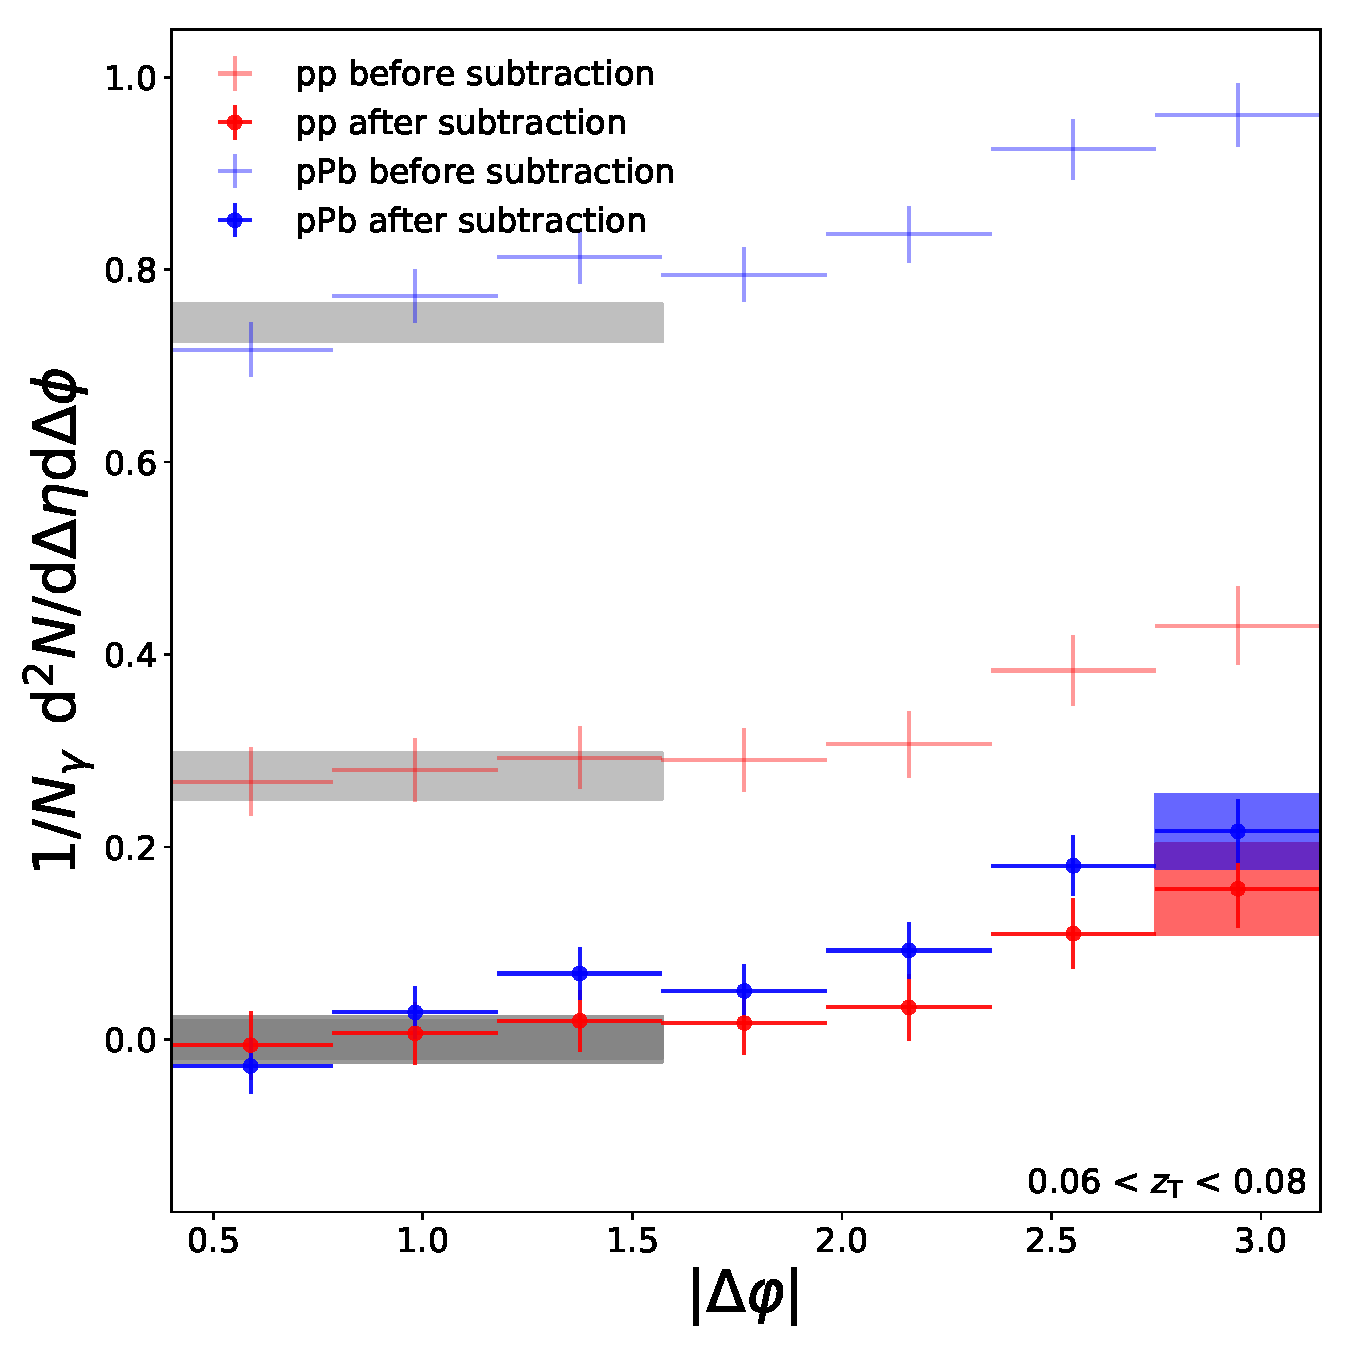
\includegraphics[width = 0.24 \textwidth]{G-H_New/Befor_After_UE_pp-pPb_pT_0_zT_0.pdf}
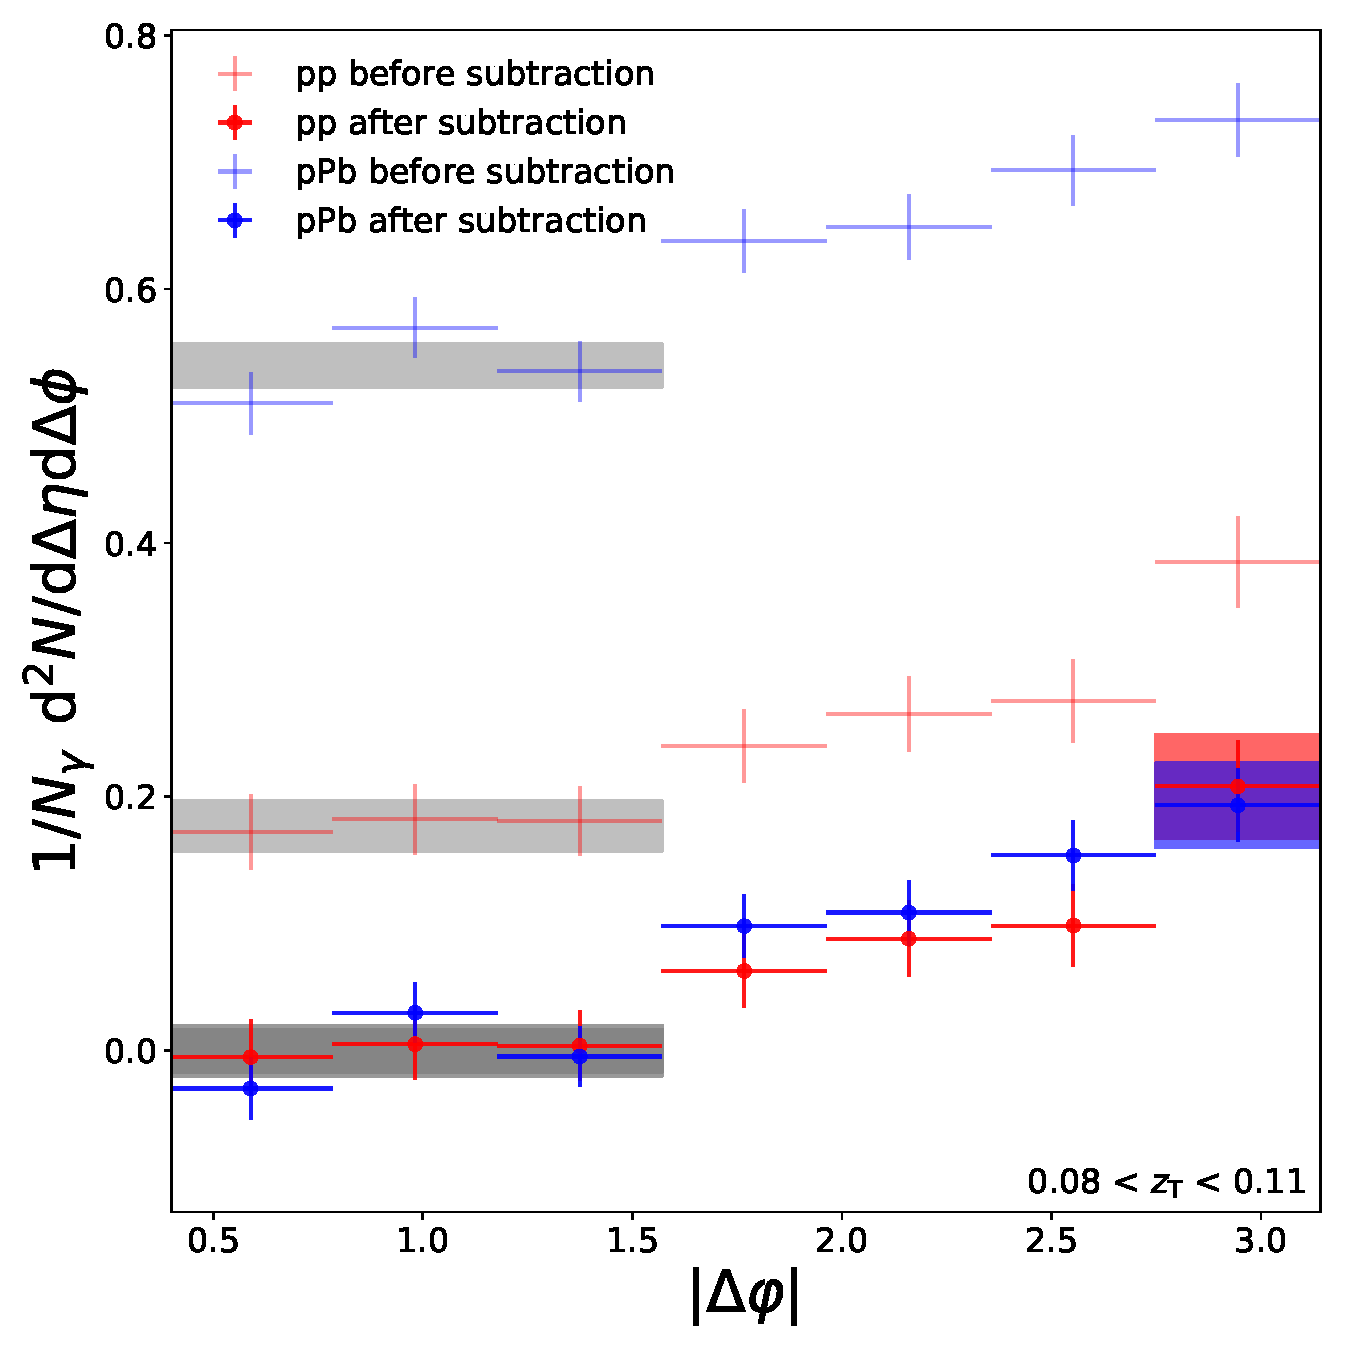
\includegraphics[width = 0.24 \textwidth]{G-H_New/Befor_After_UE_pp-pPb_pT_0_zT_1.pdf}
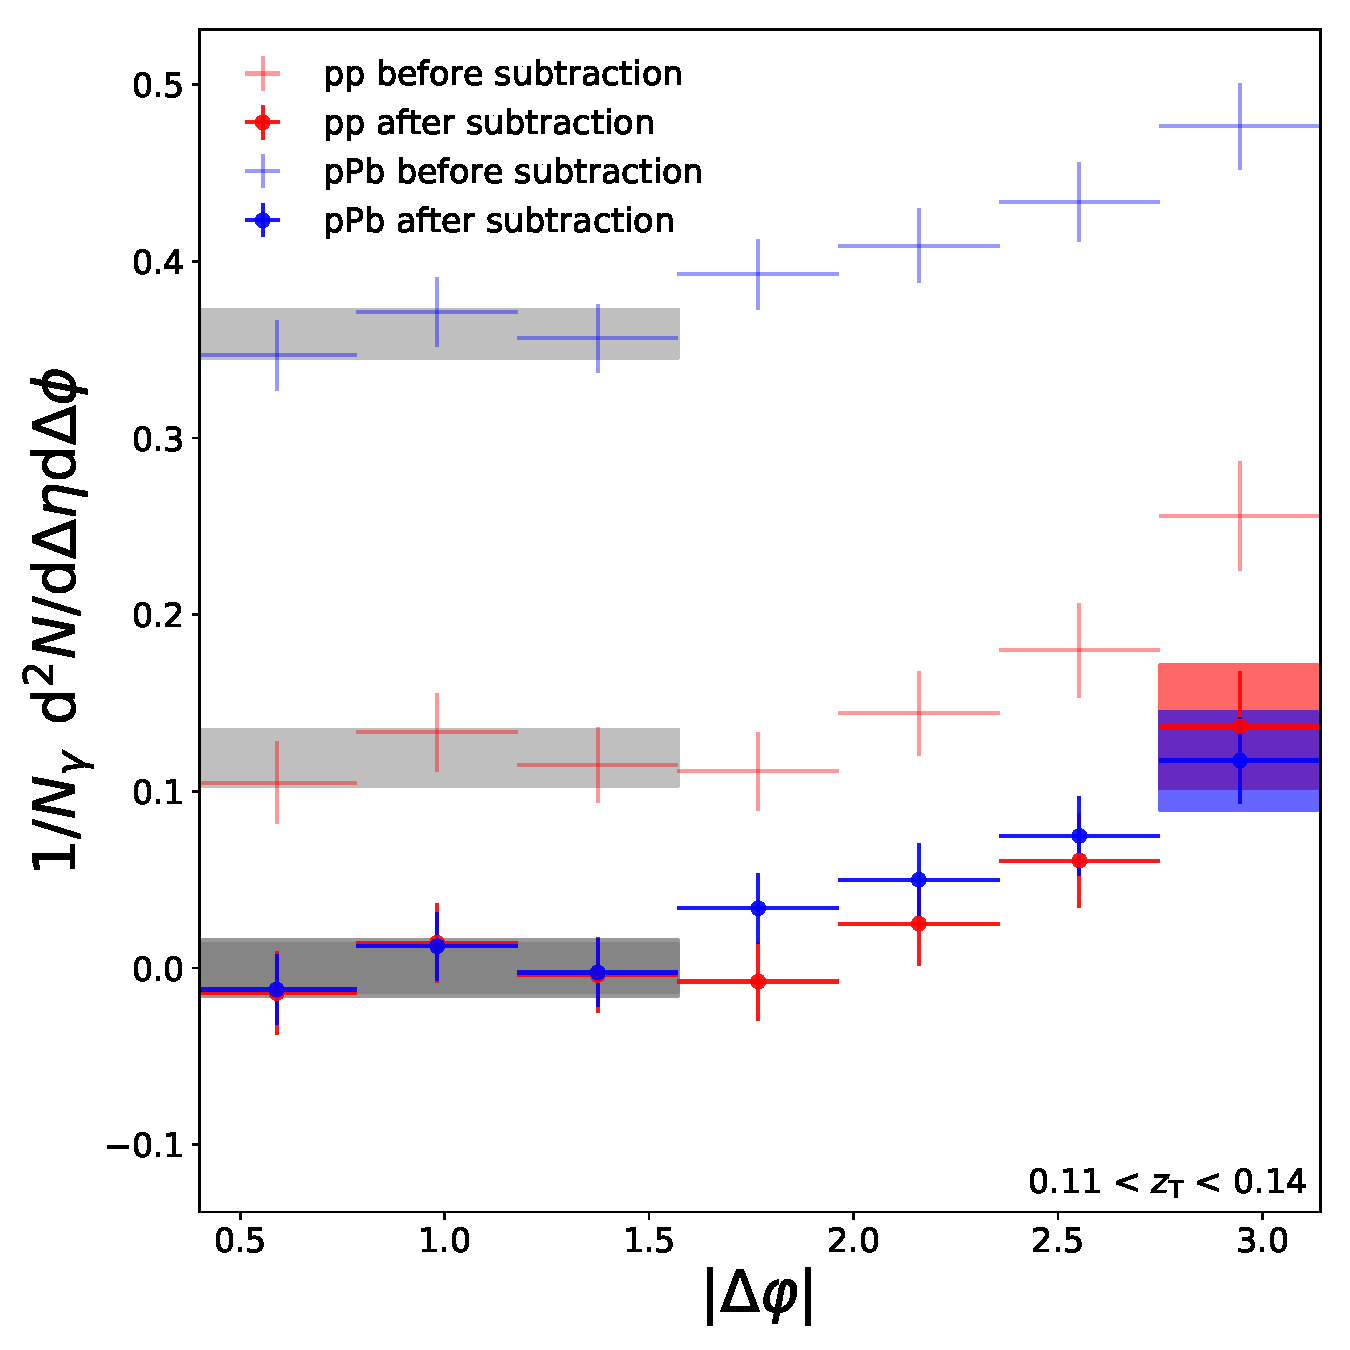
\includegraphics[width = 0.24 \textwidth]{G-H_New/Befor_After_UE_pp-pPb_pT_0_zT_2.pdf}
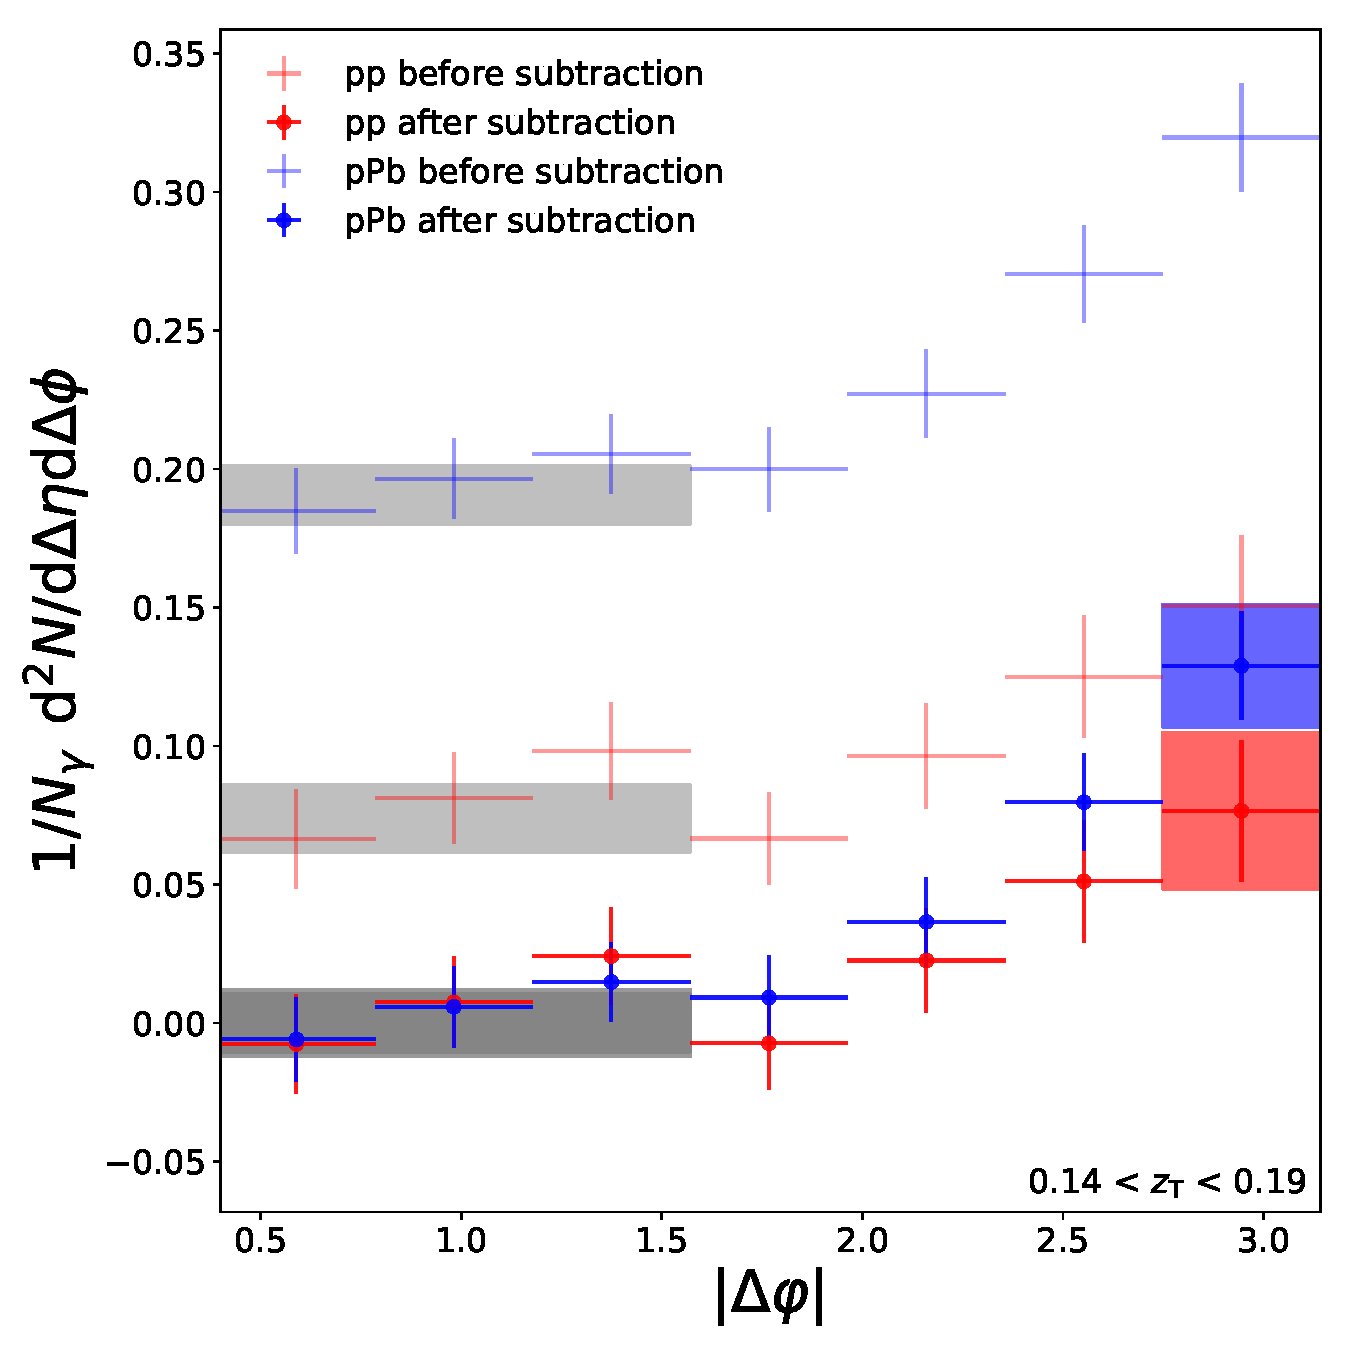
\includegraphics[width = 0.24 \textwidth]{G-H_New/Befor_After_UE_pp-pPb_pT_0_zT_3.pdf}
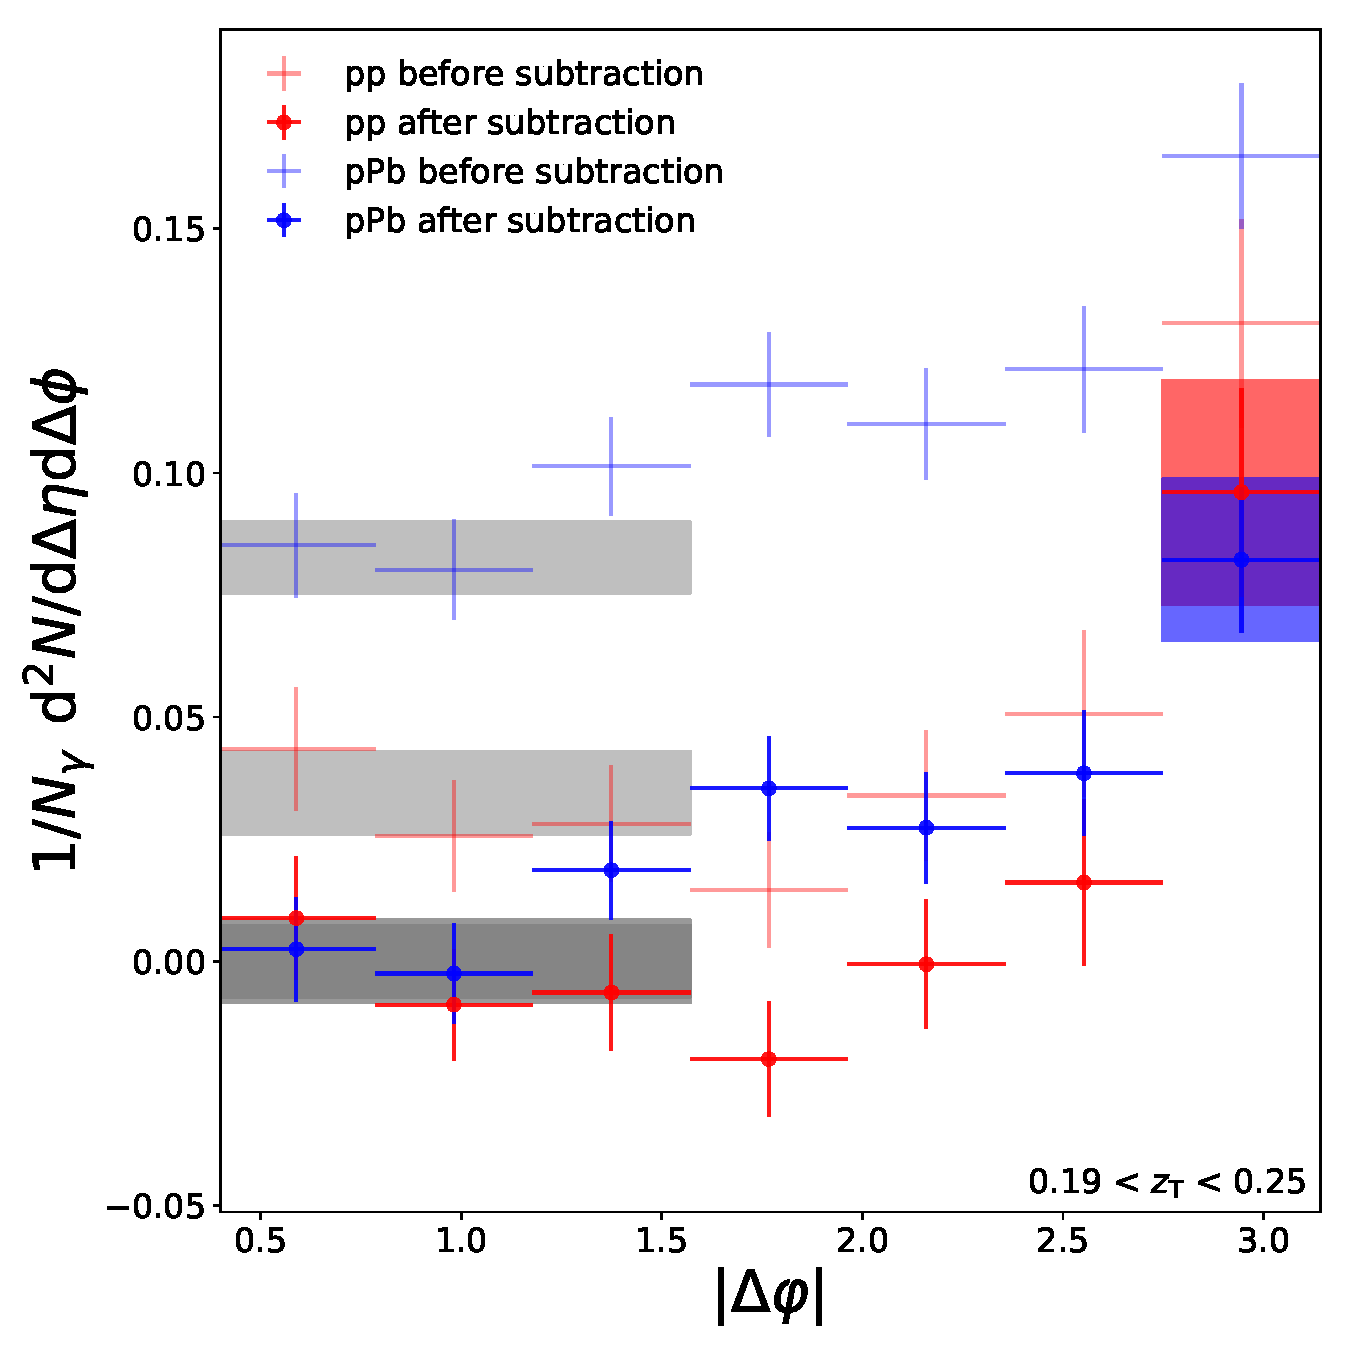
\includegraphics[width = 0.24 \textwidth]{G-H_New/Befor_After_UE_pp-pPb_pT_0_zT_4.pdf}
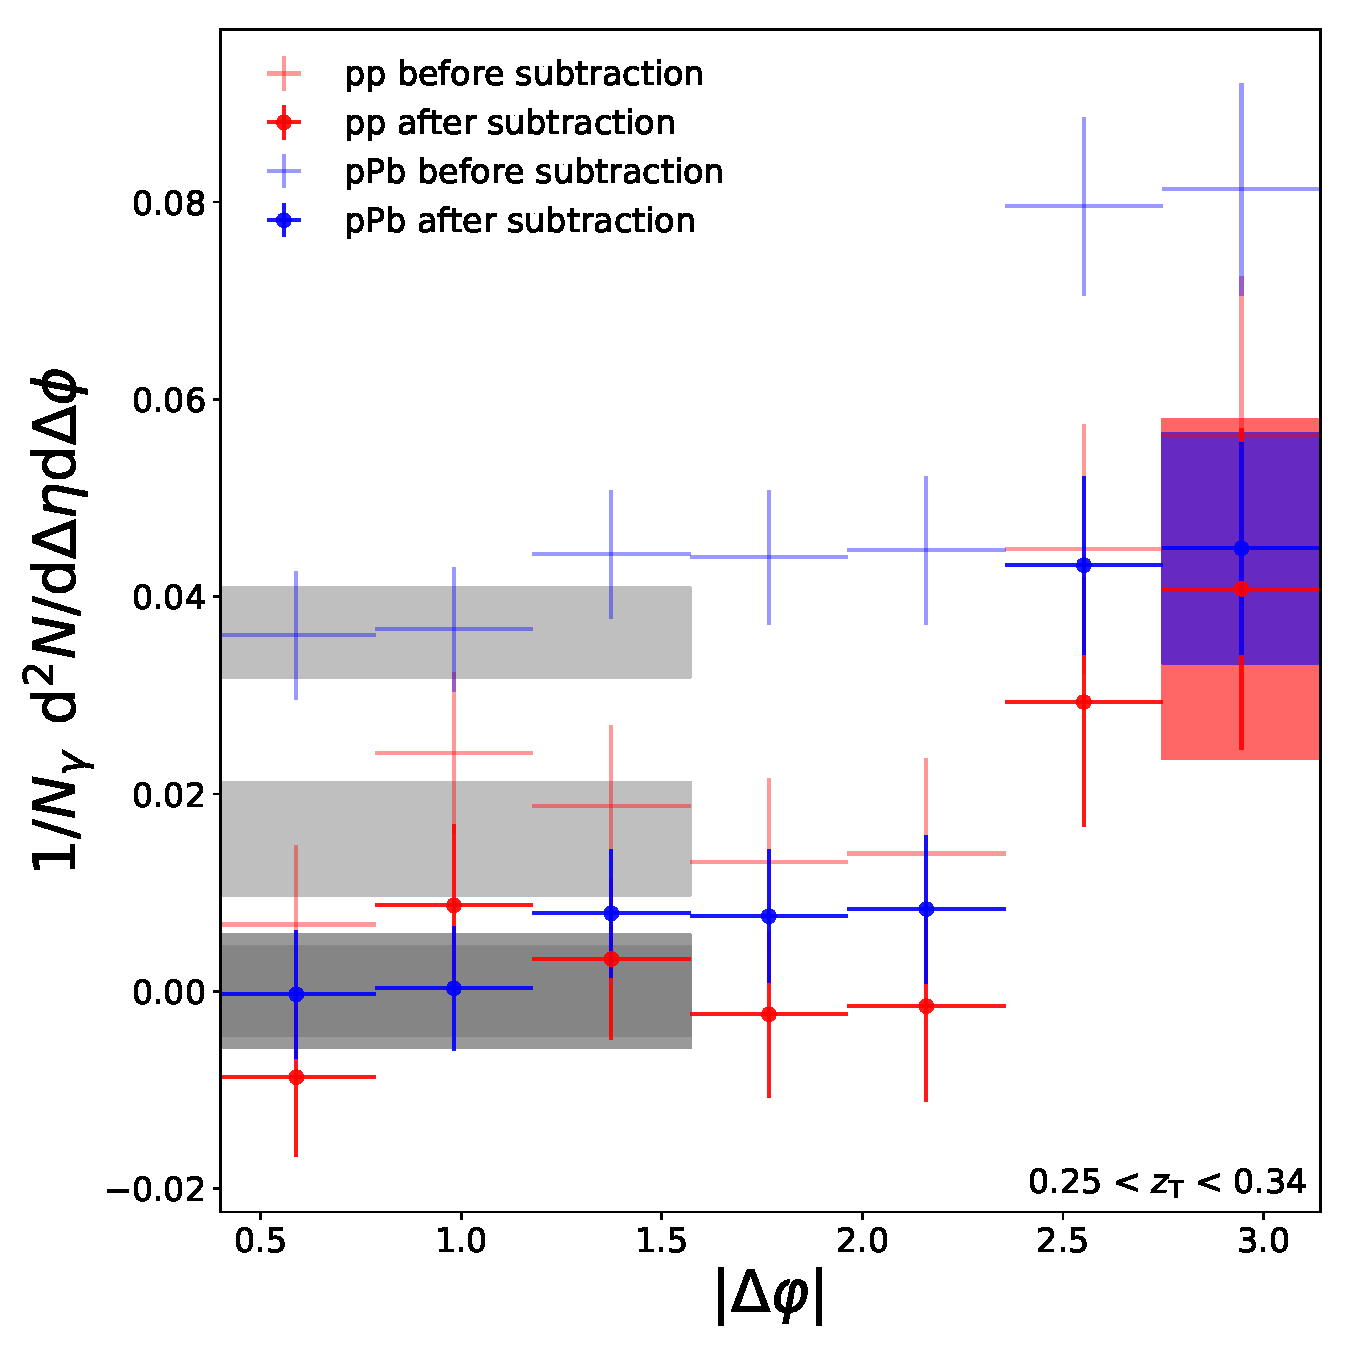
\includegraphics[width = 0.24 \textwidth]{G-H_New/Befor_After_UE_pp-pPb_pT_0_zT_5.pdf}
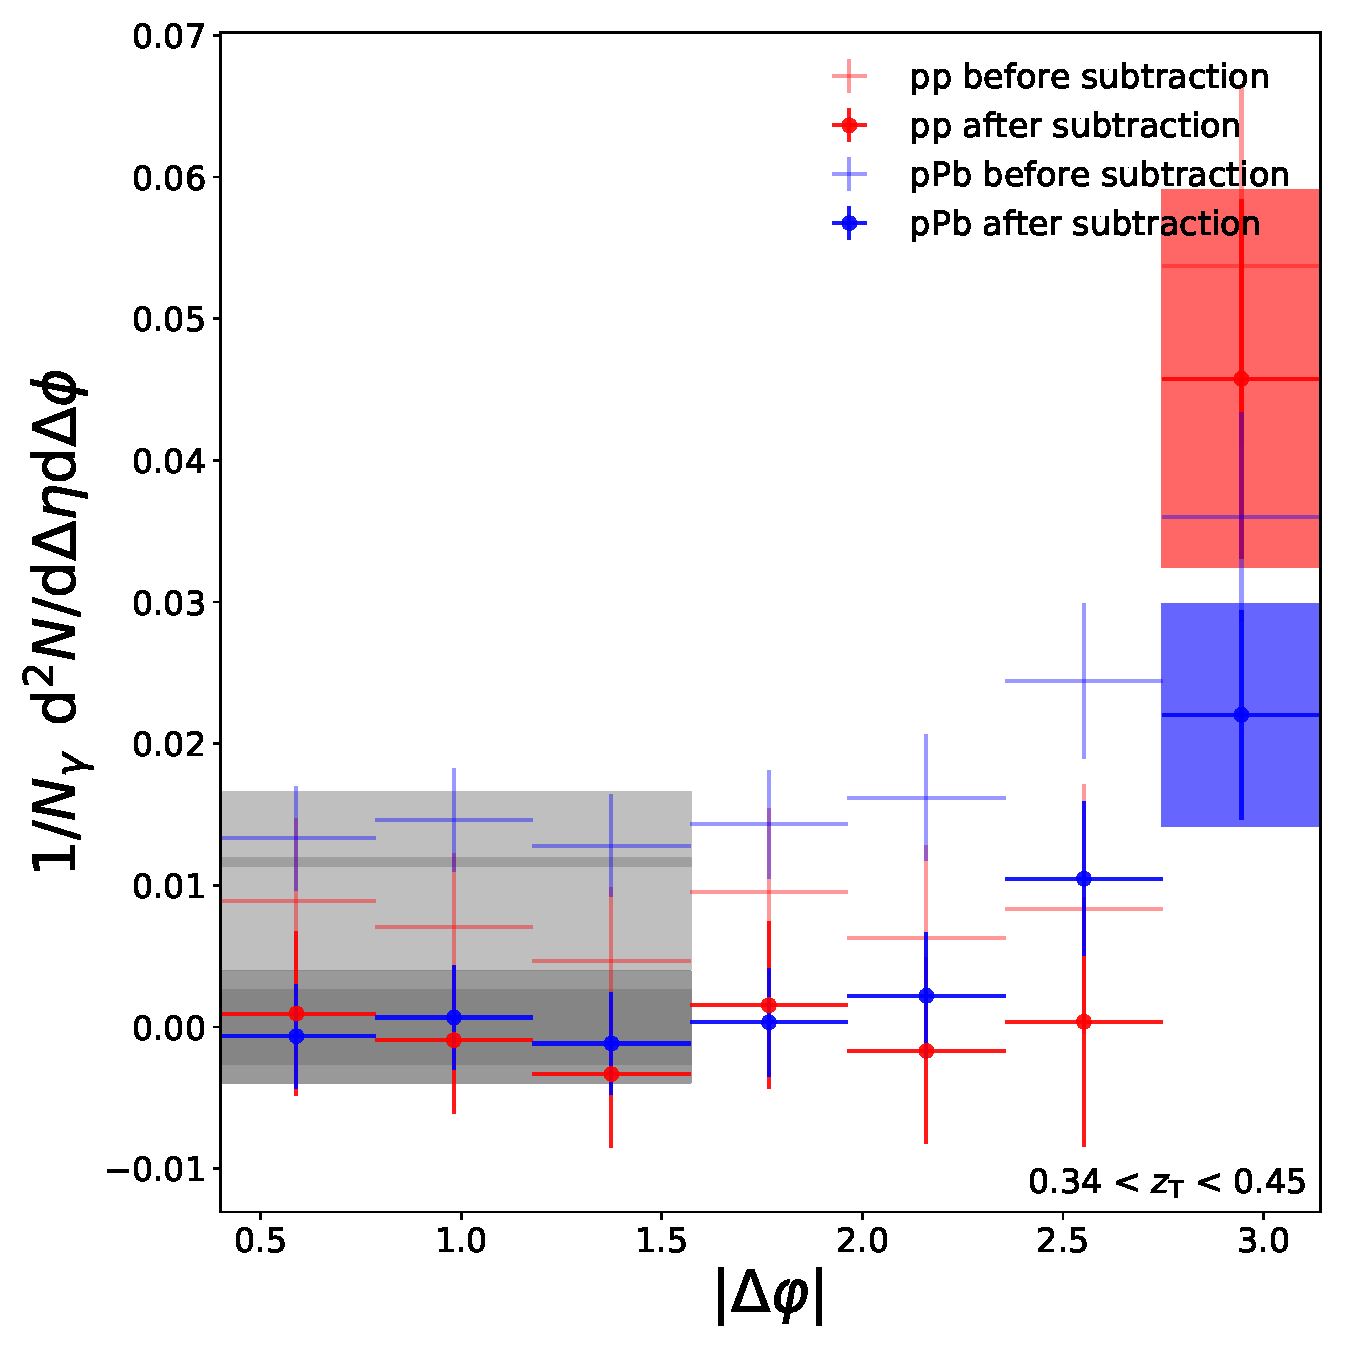
\includegraphics[width = 0.24 \textwidth]{G-H_New/Befor_After_UE_pp-pPb_pT_0_zT_6.pdf}
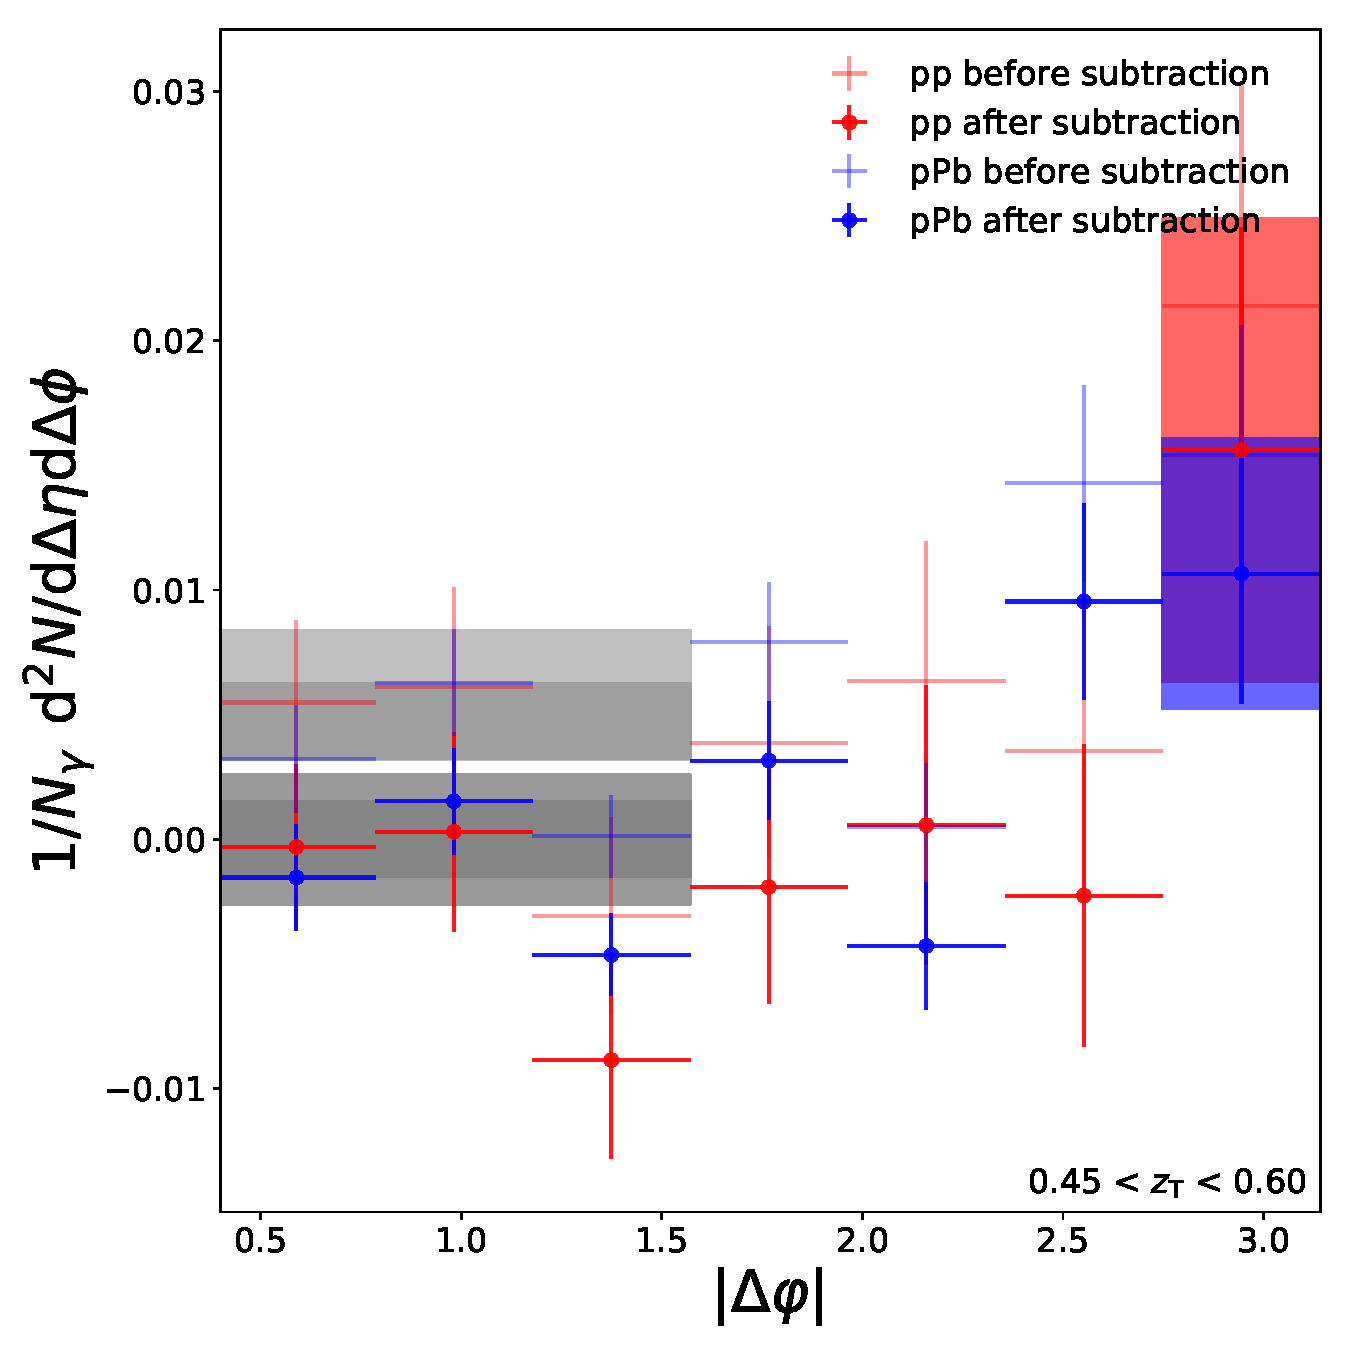
\includegraphics[width =0.24 \textwidth]{G-H_New/Befor_After_UE_pp-pPb_pT_0_zT_7.pdf}
\caption{Correlation functions in pp (red) and \pPb~(blue) before and after pedestal subtraction. The light grey bands represent the ZYAM estimates, while the dark gray bands represent the near side average after subtraction. The colored bands represent the away side average after pedestal subtraction}
\label{fig:BF_UE_zT_second}
\end{sidewaysfigure}

\subsubsection{Study of neutral energy in isolation variable using \textsc{Pythia8}}

In our analysis, we chose to construct the isolation variable using only charged-particles. In principle, we could have added neutral particles as well in the isolation definition. However, that would have limited the acceptance our our measurement. For example, the recent ALICE isolated photon paper~\cite{Acharya:2019jkx} restricted the pseudorapidity of the $\gammaiso$ to $|\eta|<0.27$ to ensure a good containment of the isolation cone that has a radius of $R=0.4$ (the EMCal acceptance is $|\eta|<0.67$). An acceptance limitation would have a large impact of this analysis so we chose to use only ``charged-only" isolation. This is not different than several ALICE jet analyses that report ``charged-only" jets and not ``full-jets". 

We use \textsc{Pythia8} events to estimate what difference would it make in our measurement to include neutral-particles in our isolation variable. Figure~\ref{fig:PythiaNeutralIsolation} shows the comparison of the prompt-photon hadron correlations according to \textsc{Pythia8} when using no isolation requirement; with an isolation variable based on charged particles (this is what we use in our analysis); and with an isolation variable based on both charged-particles and neutral particles. In all cases, the charged-particles and neutral particles are final-state particles and have $\pt>150$ MeV/$c$ and $|\eta|<0.8$. We observe that there is no significant difference between the selection of 1.5 \GeVc~based on charged particles and the selection based on 2.0 \GeVc~based on charged and neutral particles. We conclude therefore than our $\iso<1.5$ \GeVc~selection is enough to suppress the near-side peak in the correlation functions coming from fragmentation photons, and that using neutral-particles in our isolation variable would not yield any significant improvement.

\begin{sidewaysfigure}[ht]
\centering
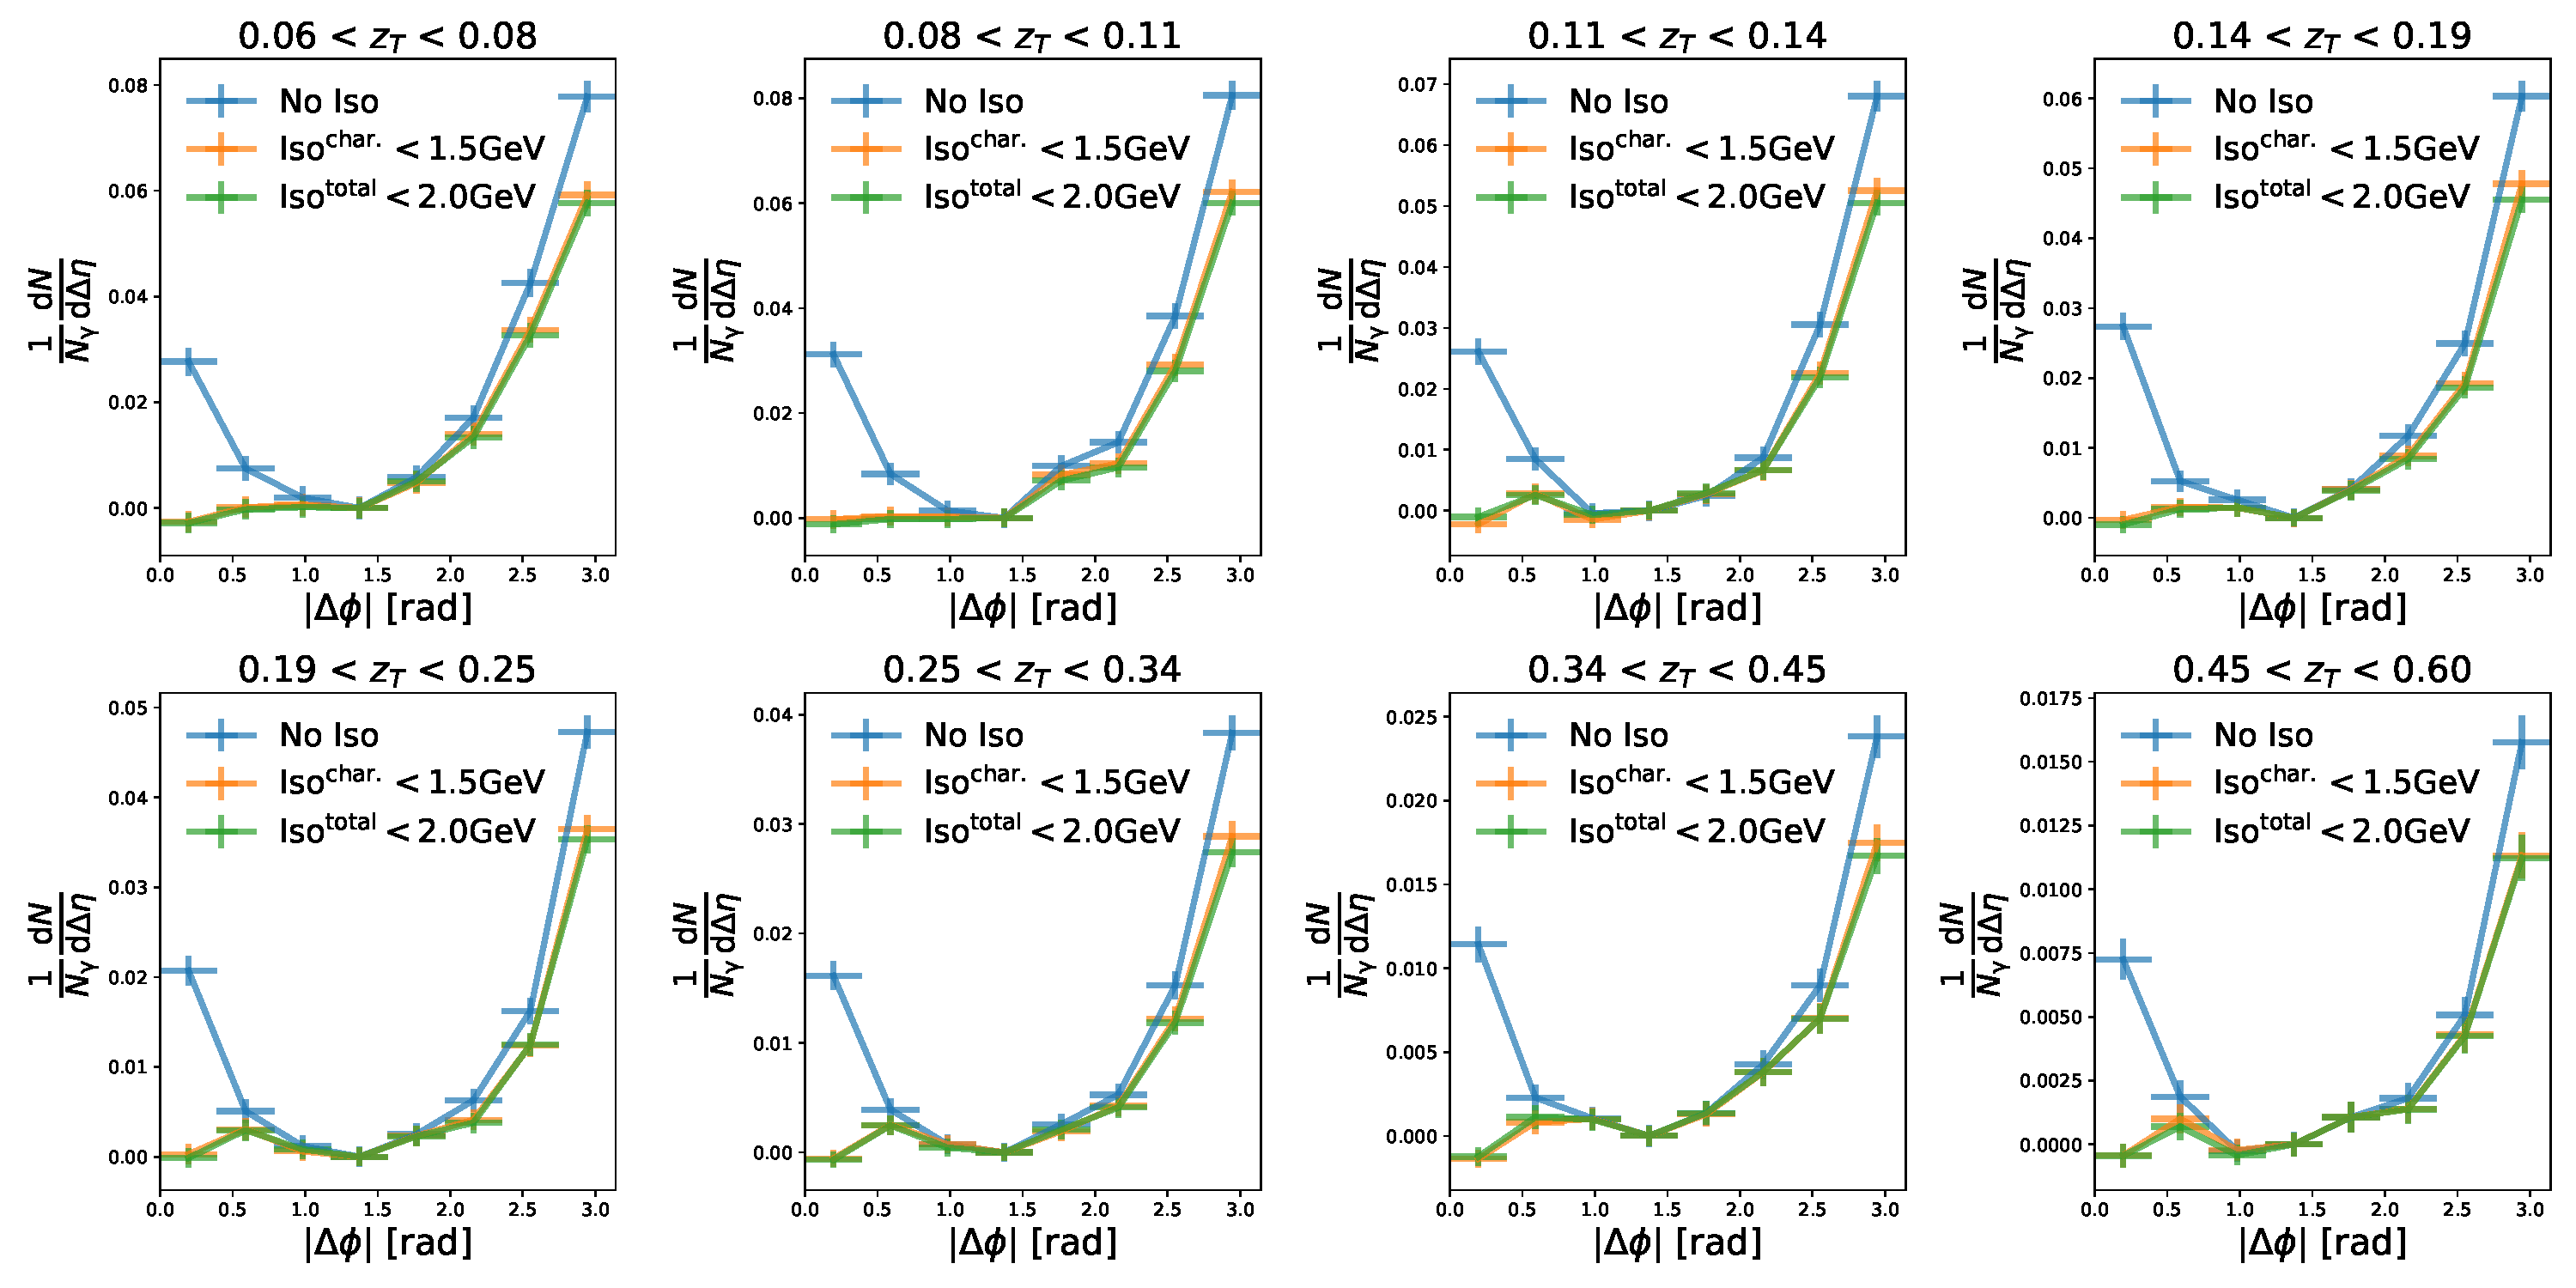
\includegraphics[width = 1.0 \textwidth]{PythiaStudyNeutralIso}
\caption{Correlation function between prompt photons and hadrons from \textsc{Pythia8} for various \zt~bins. Three selections on the prompt photons based on isolation are presented: no isolation (blue); $\iso< 1.5$\GeVc~that considers only charged-particles (orange); and $\iso<2.0$ \GeVc~that considers both charged and neutral particles (green). In all cases, the uncorrelated background has been subtracted using the ZYAM method. The error bar represent statistical uncertainty only. }
\label{fig:PythiaNeutralIsolation}
\end{sidewaysfigure}


\subsubsection{Estimate of impact of acceptance difference between pp and \pPb~due to boost}
\label{sec:bootstudy}

In this section, we estimate the impact of the acceptance difference between pp and \pPb~data that arises due to the boost in \pPb~data. The boost in \pPb~data arises due to the energy difference between the proton and lead beam, and it amounts to a rapidity difference of $\Delta y = 0.47$  in the proton-going direction. That means that in \pPb~collisions, our lab acceptance for photons that is $-0.67<\eta<0.67$ corresponds to $-0.2<\eta<1.14$ in the center-of-mass frame, whereas our charged-particle acceptance of $-0.8<\eta<0.8$ corresponds to $-0.33<\eta<1.27$  in the center-of-mass frame. 

We use \textsc{Pythia8} events to estimate what is the difference between \gammaiso--hadron correlations with the acceptance of $\gammaiso$ and charged particles  $-0.20<\eta<1.14$ and $-0.33<\eta<1.27$ instead of the nominal ranges of $-0.67<\eta<0.67$ and $-0.8<\eta<0.8$. This is shown in Figure~\ref{fig:PythiaBoostStudy}. We observe that with boosted acceptance, the $\gammaiso$--hadron correlation of about 5$\%$ lower than with the nominal acceptance, irrespective of \zt~range. For illustration purposes, we also show the impact of a boost of $\Delta y =1.0$, which shows a decrease of about 15$\%$  with respect to the nominal acceptance, irrespective of \zt~range. 

\begin{sidewaysfigure}[ht]
\centering
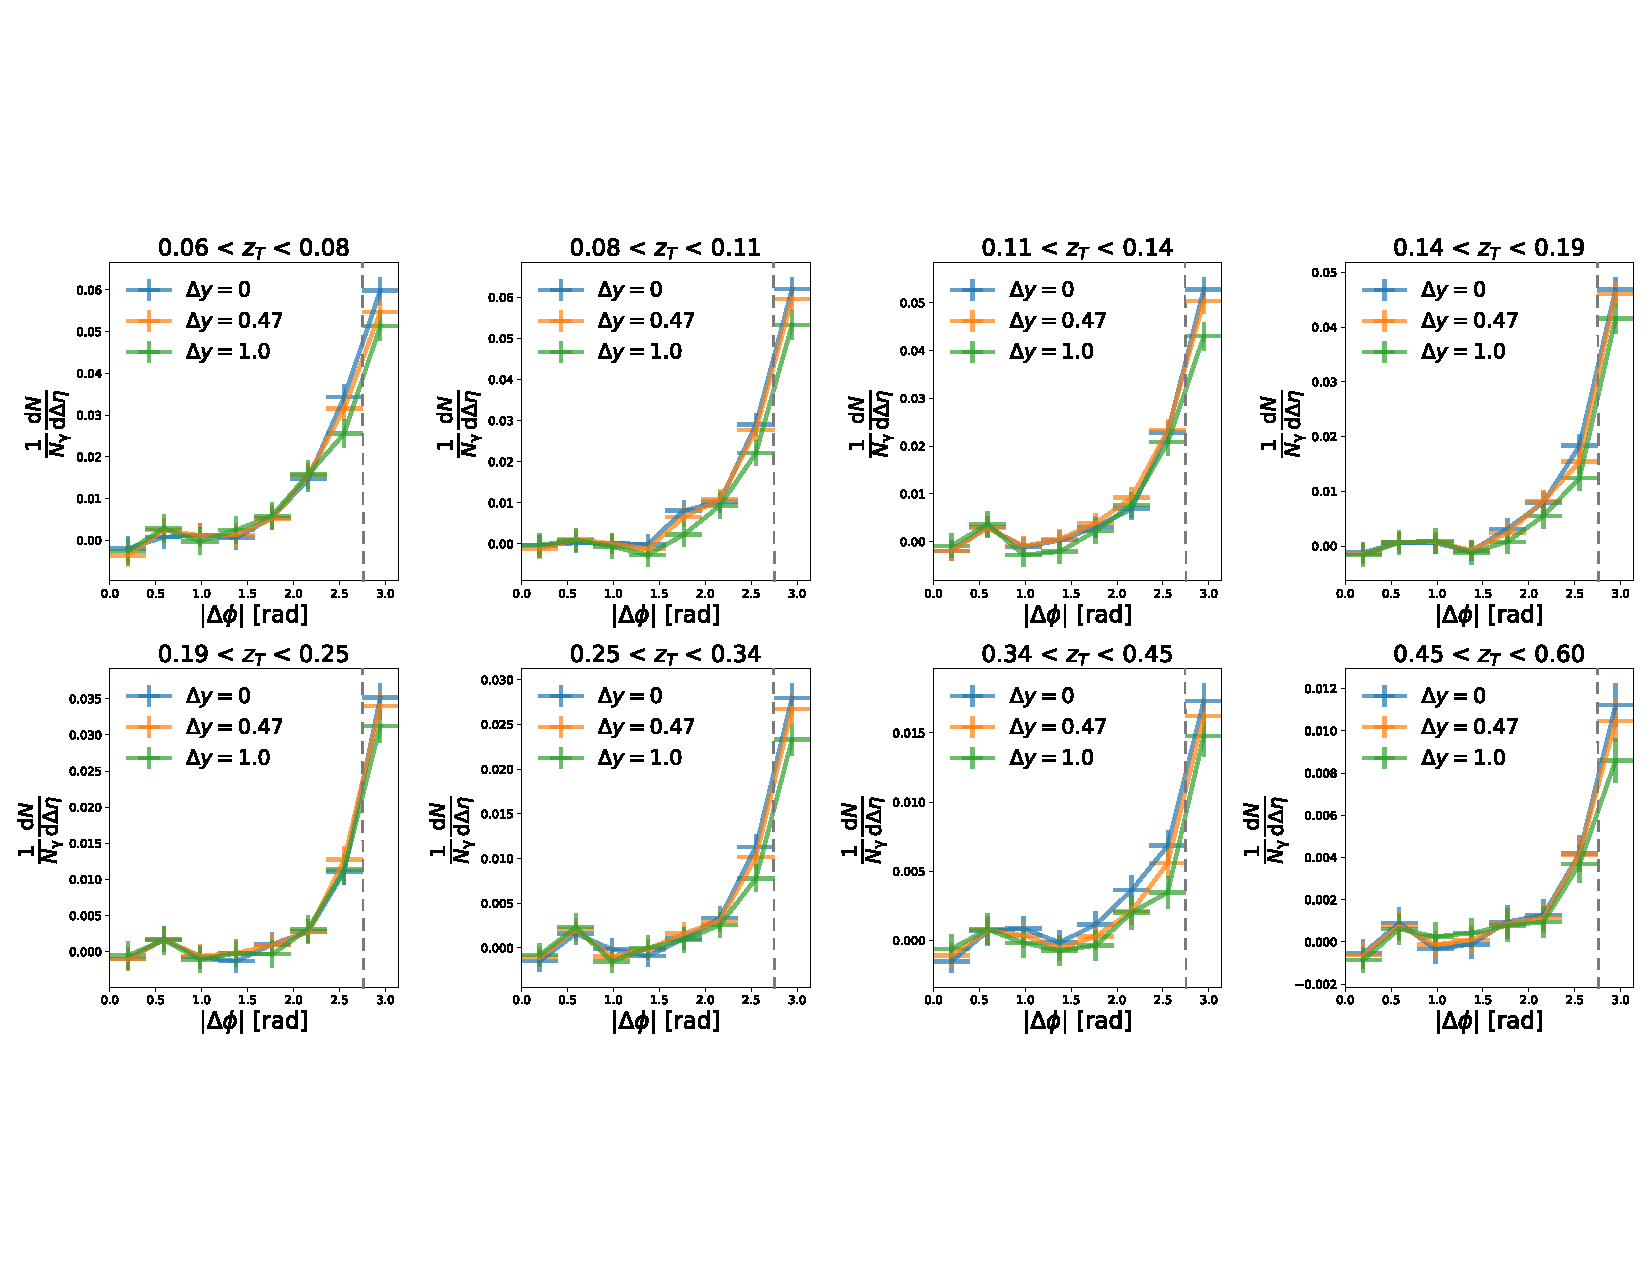
\includegraphics[width = 1.0 \textwidth]{PythiaStudyBoost_wLines.pdf}
\caption{Correlation function between isolated prompt photons and hadrons from \textsc{Pythia8} for various \zt~bins. The nominal result ($\Delta y =0$, in blue) is compared with results obtained with a kinematic selection that mimics the boost of \pPb~data (orange). For illustration purposes, we show the impact of a boost that is larger than the one of \pPb~data ($\Delta y = 1.0$ in green). The dashed lines at $\varphi = \frac{7\pi}{8} $ indicates the integration window used to obtain the away side yields.}
\label{fig:PythiaBoostStudy}
\end{sidewaysfigure}

The chosen integration window (dashed lines) in the figure above makes it clear what effect this may have on the final away side yields. We thus conclude that the effect of acceptance mismatch in our analysis is limited due to the relatively small boost of $\Delta y = 0.47$ and the limited acceptance of EMCal and ITS, which even with boost is within mid-rapidity region where the cross-sections do not change drastically. 














%%%%%%%%%%%%%%%%%%%%%%

%\subsection{$\chi^2$ Test and p-values}






%\subsection{Combining Trigger Photon \pt bins}
%The analysis is carried out independently in different \gammaiso-\pt bins. The measurement of the fragmentation is compatible in each bin, Figure {ratio of each bin to average}\ref{}. As a result, the measurement in each bin is combined using a weighted average.  The inverse relative uncertainty in each \zt bin is used as the weight to obtain an average over all \gammaiso-\pt bins:

%\begin{eqnarray}
%	&A = \frac{\sum_{i=1}^{\mathrm{N}\ z_\mathrm{T} Bins} w_i x_i}{\sum_{i=1}^{n} w_i}\\
%	&w_i = \frac{1}{\sigma_i^2}\\
%	&\sigma_i = \sqrt{\sigma_{i,stat_{rel}}^2 + \sigma_{i,purity_{rel}}tt^2}
%\end{eqnarray}





%\subsection{Comparison of Shower Shapes}
%\label{sec:FF_Shower}

%We repeat the analysis using $\lambdasquare$ and compare to the results obtained using the neural net. Figure \ref{ff_shower} compares the integrated correlation functions, and shows a comparison of pPb/pp ratios between using the two shower shapes.

%\begin{figure}[h]
%\center
%\includegraphics[width=0.9\textwidth]{GammaHadron/Shower_FFunction.pdf}
%%\includegraphics[width=0.475\textwidth]{GammaHadron/NN_L_FFunction.pdf}
%\caption{Comparison $\gammaiso$-tagged Fragmentation function of pp and pPb data between $\lambdasquare$ and the neural net as the shower shape.}
%\label{ff_shower}
%\end{figure}

%Figure \ref{ff_shower} shows good agreement between results using the two different shower shapes, and demonstrates that the effective difference between tho two shower shapes for this analysis is the purity of the signal region as described in section \ref{sec:purity}.



%%%% SR BR UE TABLE %%%%
%\begin{table}
%   \centering
%      \caption{Summary of UE-pedestal estimate with $\Delta\eta$ and ZYAM method for various $\zt$ bins in pp. The background estimate is shown in units of pairs per trigger. The uncertainty quoted is statistical only. } 
%   \begin{tabular*}{1.0\columnwidth}{@{\extracolsep{\fill}}lcccc@{}}
%    \hline
%  $\zt$ interval   & LE Signal Region & LE Background Region & ZYAM Signal Region & ZYAM Background Region  \\
%%  0.05--0.08 & 0.177 $\pm$ 0.007 & 0.182$\pm$ 0.005 & 0.193 $\pm$ 0.004 & 0.194 $\pm$ 0.003  \\
%%    0.08--0.12 & 0.121 $\pm$ 0.006 & 0.122$\pm$ 0.004 & 0.123 $\pm$ 0.003 & 0.130$\pm$ .002\\
% 0.12--0.18 & 0.061 $\pm$ 0.004 & 0.061$\pm$ 0.003 & 0.064 $\pm$ 0.002 & 0.065$\pm$ 0.002\\
%  0.18--0.28 & 0.025 $\pm$ 0.003 & 0.023$\pm$ 0.002 & 0.025 $\pm$ 0.001 & 0.026$\pm$ 0.001\\
%    0.28--0.42 & 0.007 $\pm$ 0.001 & 0.008$\pm$ 0.001 & 0.010 $\pm$ 0.001 & 0.009$\pm$ 0.001\\
%        0.42--0.65 & 0.003 $\pm$ 0.002 & 0.005$\pm$ 0.002 & 0.003 $\pm$ 0.001 & 0.003$\pm$ 0.001\\
%       \hline 
%   \end{tabular*}
%   \label{tab:UEsummary}
%\end{table}


%Table~\ref{tab:UEsummary} shows the resulting UE-pedestal estimate for various $\zt$ bins in pp and p--Pb data. The p--Pb estimates are roughly 2 times larger than the corresponding pp ones. This is consistent with the median transverse density estimates presented in Section~\ref{sec:UEsubtraction}. The statistical errors in the UE-pedestal estimates are taken as a systematic uncertainty in the final correlation function.
			
% DOING BR subtraction first, no longer applicable:
			
%The uncorrelated background is by definition independent of the trigger cluster shape. This is verified by the agreement between the uncorrelated background estimates from the two shower shape regions. 
%Consequently,
%we average the large $\Delta\eta$ uncorrelated background estimate from 
%the single photon signal and background DNN
%
%regions and subtract that value from both correlation functions. This ensures that the UE estimate is the same for both regions and reduces the statistical uncertainty in the estimate of the uncorrelated background; this statistical uncertainty on the uncorrelated background is taken as a systematic uncertainty in the final correlation. Tables \ref{tab:UEsummary} to \ref{tab:pPb_UE_Average} summarize the UE estimate in the two shower shape regions.
%
%Figure~\ref{OverlayppandPbafterUEsubtraction} shows the UE-subtracted correlation functions in pp and p--Pb data. The difference in the near side $\Delta\varphi$ region indicates that the isolation performs differently in the two systems, which is a result of the different UE in the two systems. The two systems are in reasonable agreement in the away side $\Delta\varphi$ regions, however, in most $z_{T}$ bins. 
%bvj This agreement hints at a proper UE-subtraction. (I removed this because it sounds a bit like circular reasoning. After all, we do the comparison to see whether they are different - we don't a priori know that they are not).

%\begin{figure}	
%\center
%\includegraphics[width=0.9\textwidth]{GammaHadron/pp_pPb_MC_Full_Sub.pdf}
%\caption{Comparison of UE-pedestal subtracted, signal region correlation functions within the region  $|\Delta\eta| < 0.6$ projected onto the $\Delta\varphi$-axis in pp and p+pPb. Vertical error bars represent statistical uncertainty of the data.}
%\label{OverlayppandPbafterUEsubtraction}
%\end{figure}
%
%\FloatBarrier

%\begin{table}[h]
%   \centering
%   \caption{A table of the correction factor as a function of $z_T$. The correction factor calculation includes the bin-by-bin \pt~correction from figure~\ref{fig:responseMatrixTPC} and the fake rate from figure~\ref{fig:tpcEff}.}
%   \label{tab:ZtCorrectionFactors}
%   \begin{tabular*}{1.0\columnwidth}{@{\extracolsep{\fill}}lccc@{}}
%    \hline
%     	Bin  		&Correction 	&Fake Rate\\
%       \hline
%		%0.05-0.08	&1.000			&0.018\\	
%		%0.08-0.1	&1.007			&0.018\\
%		0.12-0.18		&0.982			&0.020\\
%		0.18-0.28		&0.970			&0.022\\
%		0.28-0.42		&0.942			&0.030\\
%		0.42-0.65		&0.830			&0.085\\
%		%0.7-1.0		&0.640			&0.188\\
%\hline        
%   \end{tabular*}
%\end{table}

%\subsection{Inclusive $\gamma$ -- hadron correlations in pp}
%\label{sec:inclusivephotonhadronpp}
%We compute the correlation function, including the mixed-event correction described in Section~\ref{EventMixing}, for inclusive photons and hadrons in pp collisions. The inclusive photons are dominated by $\ydecay$ and thus this correlation is expected to be similar to di-hadron correlations. Figure~\ref{pp_2D} shows the two-dimensional correlation function. 
%\begin{figure}[h]
%\center
%\includegraphics[width=0.6\textwidth]{GammaHadron/2D_pp_inclusive_Correlations.pdf}
%\caption{Inclusive photon-hadron correlation in $\Delta\varphi$ and $\Delta\eta$ The near side "jet peak" is observed, centered at $\Delta\eta\Delta\varphi$. The away side peak extends to large values of $\Delta\eta$, as expected.}
%\label{pp_2D}
%\end{figure}
%
%
%%Figure~\ref{fig:inclusivephotonETA} shows the $\Delta\eta$ projection for inclusive photon-hadron correlations in the region $|\Delta\varphi|<\pi/2$. This illustrates the extent of the near-side or ``jet peak'' that results from particles collimated in $\varphi$ and $\eta$. The near-side peak gets narrower as $\zt$ increases; a similar observation was previously reported in Ref \cite{PhysRevLett.119.102301}.
%%\begin{figure}
%%\center
%%\includegraphics[width=1.0\textwidth]{GammaHadron/pp_Eta_Inclusive.pdf}
%%\caption{Inclusive photon hadron correlations for different hadron $\zt$ bins in pp collisions. The near-side peak is clearly visible. The projection is taken from the $\Delta\varphi$ range of $0< \Delta\varphi < \pi/2$. The error bar represent statistical uncertainty only. The grey band represents the uncorrelated background estimated from the large $\Delta\eta$ region  $0.8<\Delta\eta<1.4$.}
%%\label{fig:inclusivephotonETA}
%%\end{figure}
%
%This informs our choice for $\Delta\eta$ range used in one method for UE-pedestal estimate described in \ref{sec:UncorrBkgnd} . We choose the range $0.8<\Delta\eta<1.2$ that is a compromise between the statistical uncertainty and limiting the influence of any near-side jet signal.
%
%Figure~\ref{fig:inclusivephoton} shows correlation functions between inclusive $\gamma$ and hadrons in pp data projected onte the $\varphi$-axis. The correlation function shows a large near-side peak and a smaller away-side peak, resembling hadron-hadron correlations, as expected since the dominant source of inclusive $\gamma$'s is $\pi^{0}$ decay. 
%
%\begin{figure}
%\center
%\includegraphics[width=1.0\textwidth]{GammaHadron/pp_Inclusive_Phi.pdf}
%\caption{Inclusive photon hadron correlations for different hadron $\zt$ bins in pp collisions.  The projection is taken from the $\Delta\eta$ range of $|\Delta\eta <0.6$. The error bar represent statistical uncertainty only.}
%\label{fig:inclusivephoton}
%\end{figure}
%
%At low $\zt$, the correlation functions exhibit a large ``pedestal'' created by the association of clusters from hard-scattering with charged particles from the underlying event (UE). We define this as the uncorrelated background and this yields a uniform $\Delta\varphi$ background (except in very high multiplicity pp events, which are very rare). The UE-pedestal decreases as $\zt$ increases, as expected since the UE is dominated by soft particles. At $\zt=0.18$ and higher, the UE-pedestal is much smaller than the away-side peak. 
%
%This illustrates that our event-mixing correlation works as intended, as there are no large deviations from an expected correlation function. (i.e, no large dips or bumps in $\Delta\varphi$) 
%
%\FloatBarrier
%\subsection{Inclusive photon--hadron correlations in p--Pb data}
%\label{sec:inclusivephotonhadronpPb}
%
%%\begin{figure}
%%\center
%%\includegraphics[width=0.9\textwidth]{GammaHadron/13def_Eta_Inclusive.png}
%%\caption{Inclusive photon hadron correlations for different hadron $\zt$ bins in p--Pb collisions.  The region $\Delta\varphi$ $< \pi/2$ is projected onto the $\Delta\eta$-axis. The error bar represent statistical uncertainty only. The grey band represent the average of the large $|\Delta\eta|$ region, which gives an estimate to the uncorrelated background.}
%%\label{fig:pPbinclusivephotonETA}
%%\end{figure}
%
%Figure~\ref{fig:pPbinclusivephotonPhi} shows correlation functions between inclusive $\gamma$'s and hadrons in p--Pb data projected onto the $\Delta\eta$ axis, integrating the $\Delta\varphi$ range of $0< \Delta\varphi < \pi/2$ . %[Slope in eta being investigated]
%
%Relative to the inclusive photon results in pp, shown in Figure \ref{fig:inclusivephoton}, these results show a much larger UE-pedestal; the pedestal maximum is 
%%bvj that is largest 
%at the lowest $\zt$ bins (where the UE is higher by about of a factor of 3 than in pp collisions). This has the consequence that the jet peak seems smaller relative to the pedestal. However, closer inspection shows that the height of the peak relative to the UE-pedestal is indeed similar in p--Pb and pp data. This will be further investigated after UE-pedestal and decay-photon backgrounds subtraction, in Section \ref{sec:UncorrBkgnd}. Figure~\ref{fig:pPbinclusivephotonPhi} shows the projection onto the $\Delta\varphi$ axis.
%
%\begin{figure}[h]
%\center
%\includegraphics[width=0.9\textwidth]{GammaHadron/13def_Inclusive_Phi.pdf}
%\caption{Inclusive photon hadron correlations for different hadron $\zt$ bins in p--Pb collisions. The region within $|\Delta\eta| < 0.6$ is projected onto the $\Delta\varphi$-axis. The vertical error bars represent statistical uncertainty only, and are extremely small here due to the high statistics for inclusive photons..}
%\label{fig:pPbinclusivephotonPhi}
%\end{figure}


%--------------------------------------------------------

%\subsection{Isolated photon -- hadron correlations in pp}
%\label{sec:isolatedphoton_pp}
%As described in Section~\ref{sec:isolation}, we apply an isolation cut within a $\gammaiso$ selection. The correlation function from $\gammaiso$-candidates and hadrons in pp collisions is shown in Figure ~\ref{fig:IsolatedPhoton}. 
%
%%\begin{figure}
%%\center
%%\includegraphics[width=1.0\textwidth]{GammaHadron/pp_Eta_2DNN.pdf}
%%\caption{$\Delta\eta$ projection of Isolated photon hadron correlations for different hadron $\zt$ bins in pp collisions. To avoid integrating the away-side jet peak, the projection is taken from the $\Delta\varphi$ range of $0< \Delta\varphi < \pi/2$. The gray band represents the uncorrelated background estimate.}
%%\label{fig:isophotonETA}
%%\end{figure}
%
%%Figure~\ref{fig:isophotonETA} shows the $\Delta\eta$ projection for isolated photons in the two shower shape regions. 
%
%%Figure \ref{pp_2D} shows a 2D inclusive photon-hadron correlation in $\Delta\varphi$ and $\Delta\eta$. The $\Delta\eta$ projections. This informs the $\Delta\eta$ regions to use for the our uncorrelated background estimate, as well as for the final correlations.
%
% The analysis procedure in this section is carried out identically for cluster-track correlations in both shower shape regions, defined in Table \ref{tab:shape_table}, before the final subtraction outlined in Equation \ref{eq:FinalSubtraction}. 
% 
% We project the correlation function onto the $\Delta\varphi$ axis within the region $|\Delta\eta|< 1.2$. The projections of the two shower shape regions after correcting for detector acceptance effects are shown in Figure \ref{fig:IsolatedPhoton}.
%
%\begin{table}[h]
%\label{rec:Shape_Summary}
%   \centering
%      \caption{Summary of shower shape regions used to discriminate between our signal and background regions after the isolation cut is applied. The plots in this section are obtained using  $\lambdasquare$ The weighted average of the purity of the signal region for clusters within  $12 < p_T < 40$ is also given, though our use of the purity is described in section \ref{sec:purity_weight} }
%   \begin{tabular*}{1.0\columnwidth}{@{\extracolsep{\fill}}|c|c|c|c|@{}}
%    \hline
%  Shower Shape Variable   & Signal Region & Background Region & Purity(weighted average) \\
%  \hline
% %     DNN  &0.55 - 0.8 & 0.0 - 0.3 & 35\% \\
%  $\sigma^2_{\mathrm{long}}$ & $<$ 0.3 &  0.4--1.0 & 27\% \\
%% $\emax$ & 0.75- 0.95 & 0.1--0.45 & 30\%\\
%       \hline 
%   \end{tabular*}
%   \label{tab:shape_table}
%\end{table}
%
%\begin{figure}[h]
%\center
%\includegraphics[width=1.0\textwidth]{GammaHadron/pp_Phi_2DNN.pdf}
%\caption{Isolated photon hadron correlations in pp. The error bar represent statistical uncertainty only. }
%\label{fig:IsolatedPhoton}
%\end{figure}
%
%As expected, the near-side peak is 
%%bvj vastly reduced, it is 
%reduced by a factor of 2 with respect to the magnitude of the near-side peak shown in Figure~\ref{fig:inclusivephoton}. It is not completely eliminated though, because the isolation criteria requires $\iso<$1.5 GeV, which 
%%bvj is the variable that is 
%computed after UE-subtraction (about 1 GeV in p--Pb collisions and {0.5 GeV} in pp collisions). Thus, a $\gammaiso$ candidate could have up to {2.5 GeV} summed $\pt$ around it. 
%
%%bvj We measure correlations of clusters and charged particles for isolated clusters in our signal and background regions, shown in Figure~\ref{fig:IsolatedPhoton}. 
%Figure~\ref{fig:IsolatedPhoton} allows comparison of correlations functions for photons in the signal and bacgkround regions.
%As shown in Section~\ref{sec:purity}, the signal region in Figure~\ref{fig:IsolatedPhoton} is comprised of about 70$\%$ background from decay photons (i.e, it has 30$\%$ purity for prompt photons). The background region is almost exclusively background from decay photons. Thus, it is not surprising that the distributions mostly agree. 
%These distributions are used with the purity to extract the true isolated photon-hadron correlations.
%
%
%\subsection{Isolated photon--hadron correlations in p--Pb}
%\label{sec:isolatedphoton_pPb}
%
%%Figure \ref{fig:pPb_Isolated_photonETA} shows the $\Delta\eta$ projection for isolated photon-hadron correlations in our two shower shape regions for p--Pb collisions. The relative flatness in $\Delta\eta$ indicates that the mixed event technique does correct for detector acceptance effects, and justifies our use of large $\Delta\eta$ to estimate the uncorrelated background as described in section \ref{sec:UncorrBkgnd}. 
%
%Figure \ref{fig:pPb_Isolated_photonphi} shows the $\Delta\varphi$ projections for the two shower shape regions. As described in the coming sections, the UE event will be subtracted in both regions, after which the background region correlation will be scaled by the purity and subtracted from the signal region correlation.
%
%%\begin{figure}
%%\center
%%\includegraphics[width=1.0\textwidth]{GammaHadron/13def_Eta_2DNN.pdf}
%%\caption{Isolated $\gamma$-h correlations for different $\zt$ bins in p--Pb. Error bars represent statistical uncertainties. Here, he region $\Delta\varphi$ $< \pi/2$ is projected onto the $\Delta\eta$-axis. The width of the grey band represent the statistical uncertainty on the average of the large $\Delta\eta$ region ($|\Delta\eta|$ greater than 0.8). }
%%\label{fig:pPb_Isolated_photonETA}
%%\end{figure}
% 
% \newpage
% 
%\begin{figure}[h]
%\center
%\includegraphics[width=1.0\textwidth]{GammaHadron/13def_Phi_2DNN.pdf}
%\caption{$\Delta\varphi$ projection of Isolated photon hadron correlations for different hadron $\zt$ bins in p--Pb collisions. The region within $|\Delta\eta| < 1.2$ is projected onto the $\Delta\varphi$-axis. The error bar represent statistical uncertainty only.}
%\label{fig:pPb_Isolated_photonphi}
%\end{figure}
%
%\FloatBarrier


%	\begin{table}[h]
%	\centering
%	\caption{Summary of systematics uncertainties affect the fragmentation function in \textbf{proton-proton}. The label of each column indicate the source of the uncertainty. The uncertainties quoted are relative.} 
%	\begin{tabular*}{1.0\columnwidth}{@{\extracolsep{\fill}}lccccc@{}}
%	\hline
%	$\zt$ interval   	& Purity (sys.) & Purity(stat.)& Shower Shape & UE Estimate 	& Tracking Efficiency \\
%	%  0.05--0.08 & 5.7\%  & 12.5\% & 5.3\% & 5.0\% \\
%	%    0.08--0.12 & 0.2\%  & 0.4\% & 2.8\% & 5.0\% \\
%	0.12--0.18 		& 25\% 	&	 6\%	& 7\%	& 3\% 		& 5\% \\
%	0.18--0.28 		& 25\% 	&	 6\%	& 6\%	& 5\% 		& 5\% \\
%	0.28--0.42 		& 25\% 	&	 6\%	& 8\%	& 4\% 		& 5\% \\
%	0.42--0.65		& 25\%	&	 6\%	& 7\%	& 8\% 		& 5\% \\
%	   \hline 
%	\end{tabular*}
%	\label{tab:pp_FF_Uncertainties}
%	\end{table}
%	
%	
%	\begin{table}[h]
%	\centering
%	\caption{Summary of systematics uncertainties affect the fragmentation function in \textbf{proton-lead} collisions. The label of each column indicates the source of the uncertainty. The uncertainties quoted are relative.} 
%	\begin{tabular*}{1.0\columnwidth}{@{\extracolsep{\fill}}lccccc@{}}
%	\hline
%	$\zt$ interval  &Purity(sys.) &Purity (stat.) &Shower Shape	&UE Estimate	&Tracking Efficiency \\
%	%  0.05--0.08 & 25\%  & 2.5\% & 5.0\% \\
%	%    0.08--0.12 & 25\%  & 2.2\% & 5.0\% \\
%		0.12--0.18 		&25\% &	 6\%	& 2\%	&4\%			&5\% \\
%	0.18--0.28 		&25\% &	 6\%	& 1\%	&3\%			&5\% \\
%	0.28--0.42 		&25\% &	 6\%	& 1\%	&5\%			&5\% \\
%	0.42--0.65 		&25\% &	 6\%	& 1\%	&8\% 			&5\% \\
%	   \hline 
%	\end{tabular*}
%	\label{tab:pPb_FF_Uncertainties}
%	\end{table}
		
%\FloatBarrier

%\subsection{PYTHIA Check on UE}

%In the example of pp collisions, the underlying event arises from multi-parton scattering from the initial collision. In the pythia plots below, we show simulations from PYTHIA 8 Monash Tune. An indication that our underlying event subtraction is working well is if our results are compatible with and without MPI turned on in pythia. Figure \ref{fig:Pythia_Toggles} shows compatible results from pythia with and without MPI.
 
%\begin{figure}
%    \centering
%    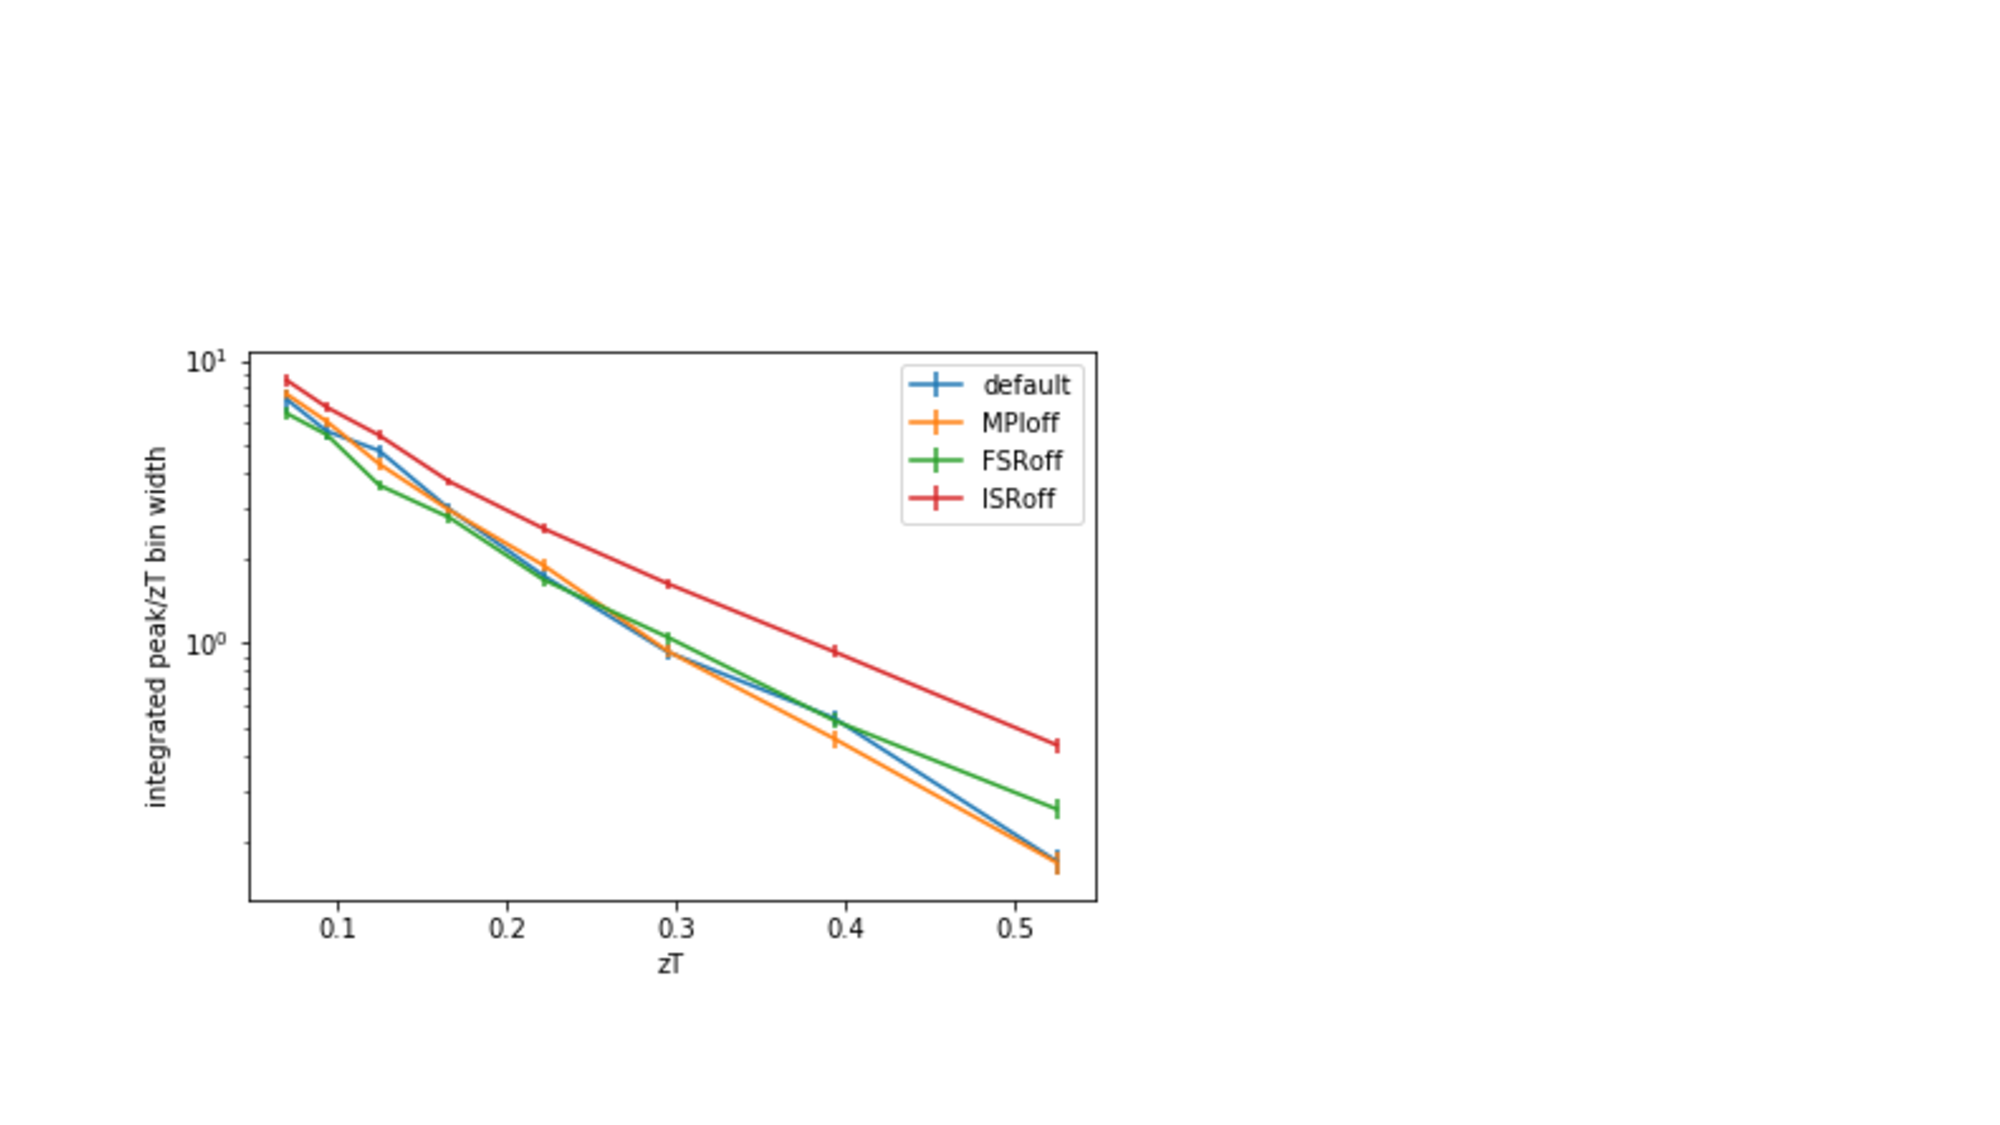
\includegraphics[width = 0.8 \textwidth]{G-H_New/Pythia_Toggles.pdf}
%    \caption{Several Interactions turned on and off for PYTHIA 8.2 Monash  simply to train the intuition and act as an additional check where appropriate. Particularly, we ses no difference in the fragmentation with and without MPI, indicating that the UE subtraction procedure is correct.}

%    \label{fig:Pythia_Toggles}
%\end{figure}

%\FloatBarrier

%\begin{figure}[h]
%\center
%\includegraphics[width=1\textwidth]{GammaHadron/NN_MC_FFunction.pdf}
%\caption{Ratio of the $\gammaiso$-tagged fragmentation function of p--Pb to pythia pp $\gamma$-jet. The black bar represents the remaining systematic+statistical uncertainties.}
%\label{ffRatio_MC}
%\end{figure}



%\begin{figure}[h]
%\center
%\includegraphics[width=0.495\textwidth]{GammaHadron/pp_FF_Fit.pdf}
%\includegraphics[width=0.495\textwidth]{GammaHadron/pPb_FF_Fit.pdf}
%\caption{Fit to fragmentation functions with an exponential in the zT range of $z_T = 0.12-0.65$.}
%\label{FF_Fit}
%\end{figure}

%\begin{equation}
%A = \frac{\sum_{i=1}^{n}w_i x_i}{\sum_{i=1}^{n}w_i} \mathrm{\ where\ weight\ } 
%\sigma_i = \sqrt{\sigma_{i,stat_{rel}}^2 + \sigma_{i,purity_{rel}}^2}
%\end{equation}

%\begin{figure}[h]
%\center
%\includegraphics[width=1\textwidth]{GammaHadron/MC_pPb_FFunction}
%\caption{Ratio of the $\gammaiso$-tagged fragmentation function of p--Pb to pythia gamma-jet simulation. The cyan error bar represents statistical only, The black bar represent the remaining systematic uncertainty. Full error propagation in process (Aug 12 2018)}
%\label{ffRatio}
%\end{figure}

%SR and BR uncertainties are summed in quadrature, with the remaining signal as the central values. 

%As an additional method for estimating the uncertainties derived from the purity, we repeat the full analysis with two different shower shape variables and use the spread in the final answer after purity-weighted subtraction to estimate the uncertainty arising from the purity measurement. The fragmentation functions in this section use the average values obtained from using the two shower shape variables,DNN and $\sigma_{long}$, with the difference from the average taken as an uncertainty. We call the source of this error simply "Shower Shape" in tables \ref{tab:pp_FF_Uncertainties} and \ref{tab:pPb_FF_Uncertainties}. A direct comparison of measurements using the two shower shapes is shown in figure \ref{ff_shower}.


%\begin{figure}[h]
%\center
%\includegraphics[width=0.495\textwidth]{GammaHadron/Ratio_Fit_0}
%\includegraphics[width=0.495\textwidth]{GammaHadron/R%atio_Fit_1}
%\caption{Fit of p--Pb/pp fragmenta.}
%\label{Ratio_Fit}
%\end{figure}

%We also take the ratio of p--Pb data to \textsc{Pythia} pp $\gamma$-jet simulation.

%To illustrate the methodology used in our correlation analyses, we begin with the simplest case, namely inclusive photon-hadron correlations in Sections~\ref{sec:inclusivephotonhadronpp} and \ref{sec:inclusivephotonhadronpPb}; Then, we describe the impact of the isolation cut in Sections ~\ref{sec:isolatedphoton_pp} and \ref{sec:isolatedphoton_pPb}.

% Each signal region cluster used in the correlation analysis is then weighted by  1/purity, where the purity obtained from the error function and that cluster's exact \pt. Background region clusters are weighted by  $\frac{1-p}{p}$, according to Equation \ref{eq:FinalSubtraction} in Section \ref{sec:decaybkgsubtraction}. 

%This cartoon is fine for thesis but not needed for analysis note 
%\begin{figure}
%    \centering
%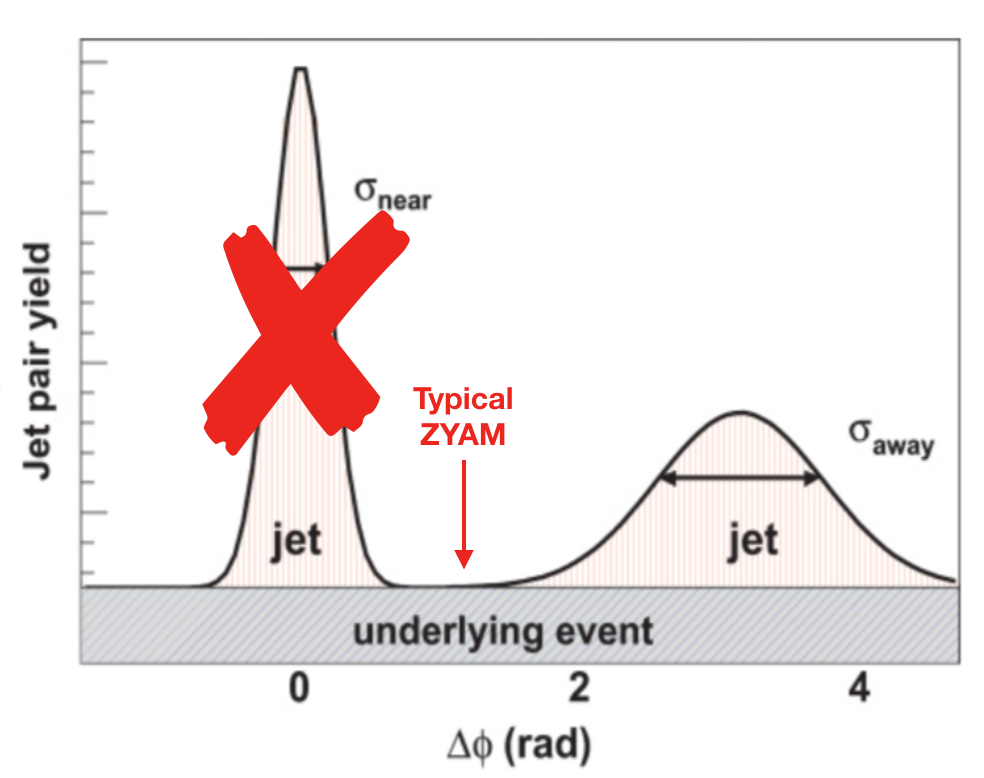
\includegraphics[width = 0.75 \textwidth]{G-H_New/Jet_Cartoon.png}
%    \caption{Isolated photon-hadron correlations do not contain the near--side jet peak present in dijet or hadron-hadron correlations. Additionally, the subtraction of $\gamma^{\mathrm{decay}}$--hadron correlations, where the photon is more likely to be part of a jet, further reduces the near-side side peak. As a result, we can use a much larger $\Delta\varphi$ range for our estimate to the underlying event}
%    \label{fig:Jet_Cartoon}
%\end{figure}
%Not needed, as it is summarized in the table
%Figures ~\ref{pp_Uncorr} and \ref{LE_ZYAM} show the two methods for all $\zt$~bins in proton-proton and proton-lead collisions respectively. The UE event estimate is roughly the same for the two shower shape regions in each $\zt$ bin. However, the UE pedestals are large, so even small differences between ZYAM and large-$\Delta\eta$ estimates can lead to noticable differences in the subtracted distribution. 
%\begin{figure}[h]
%\center
%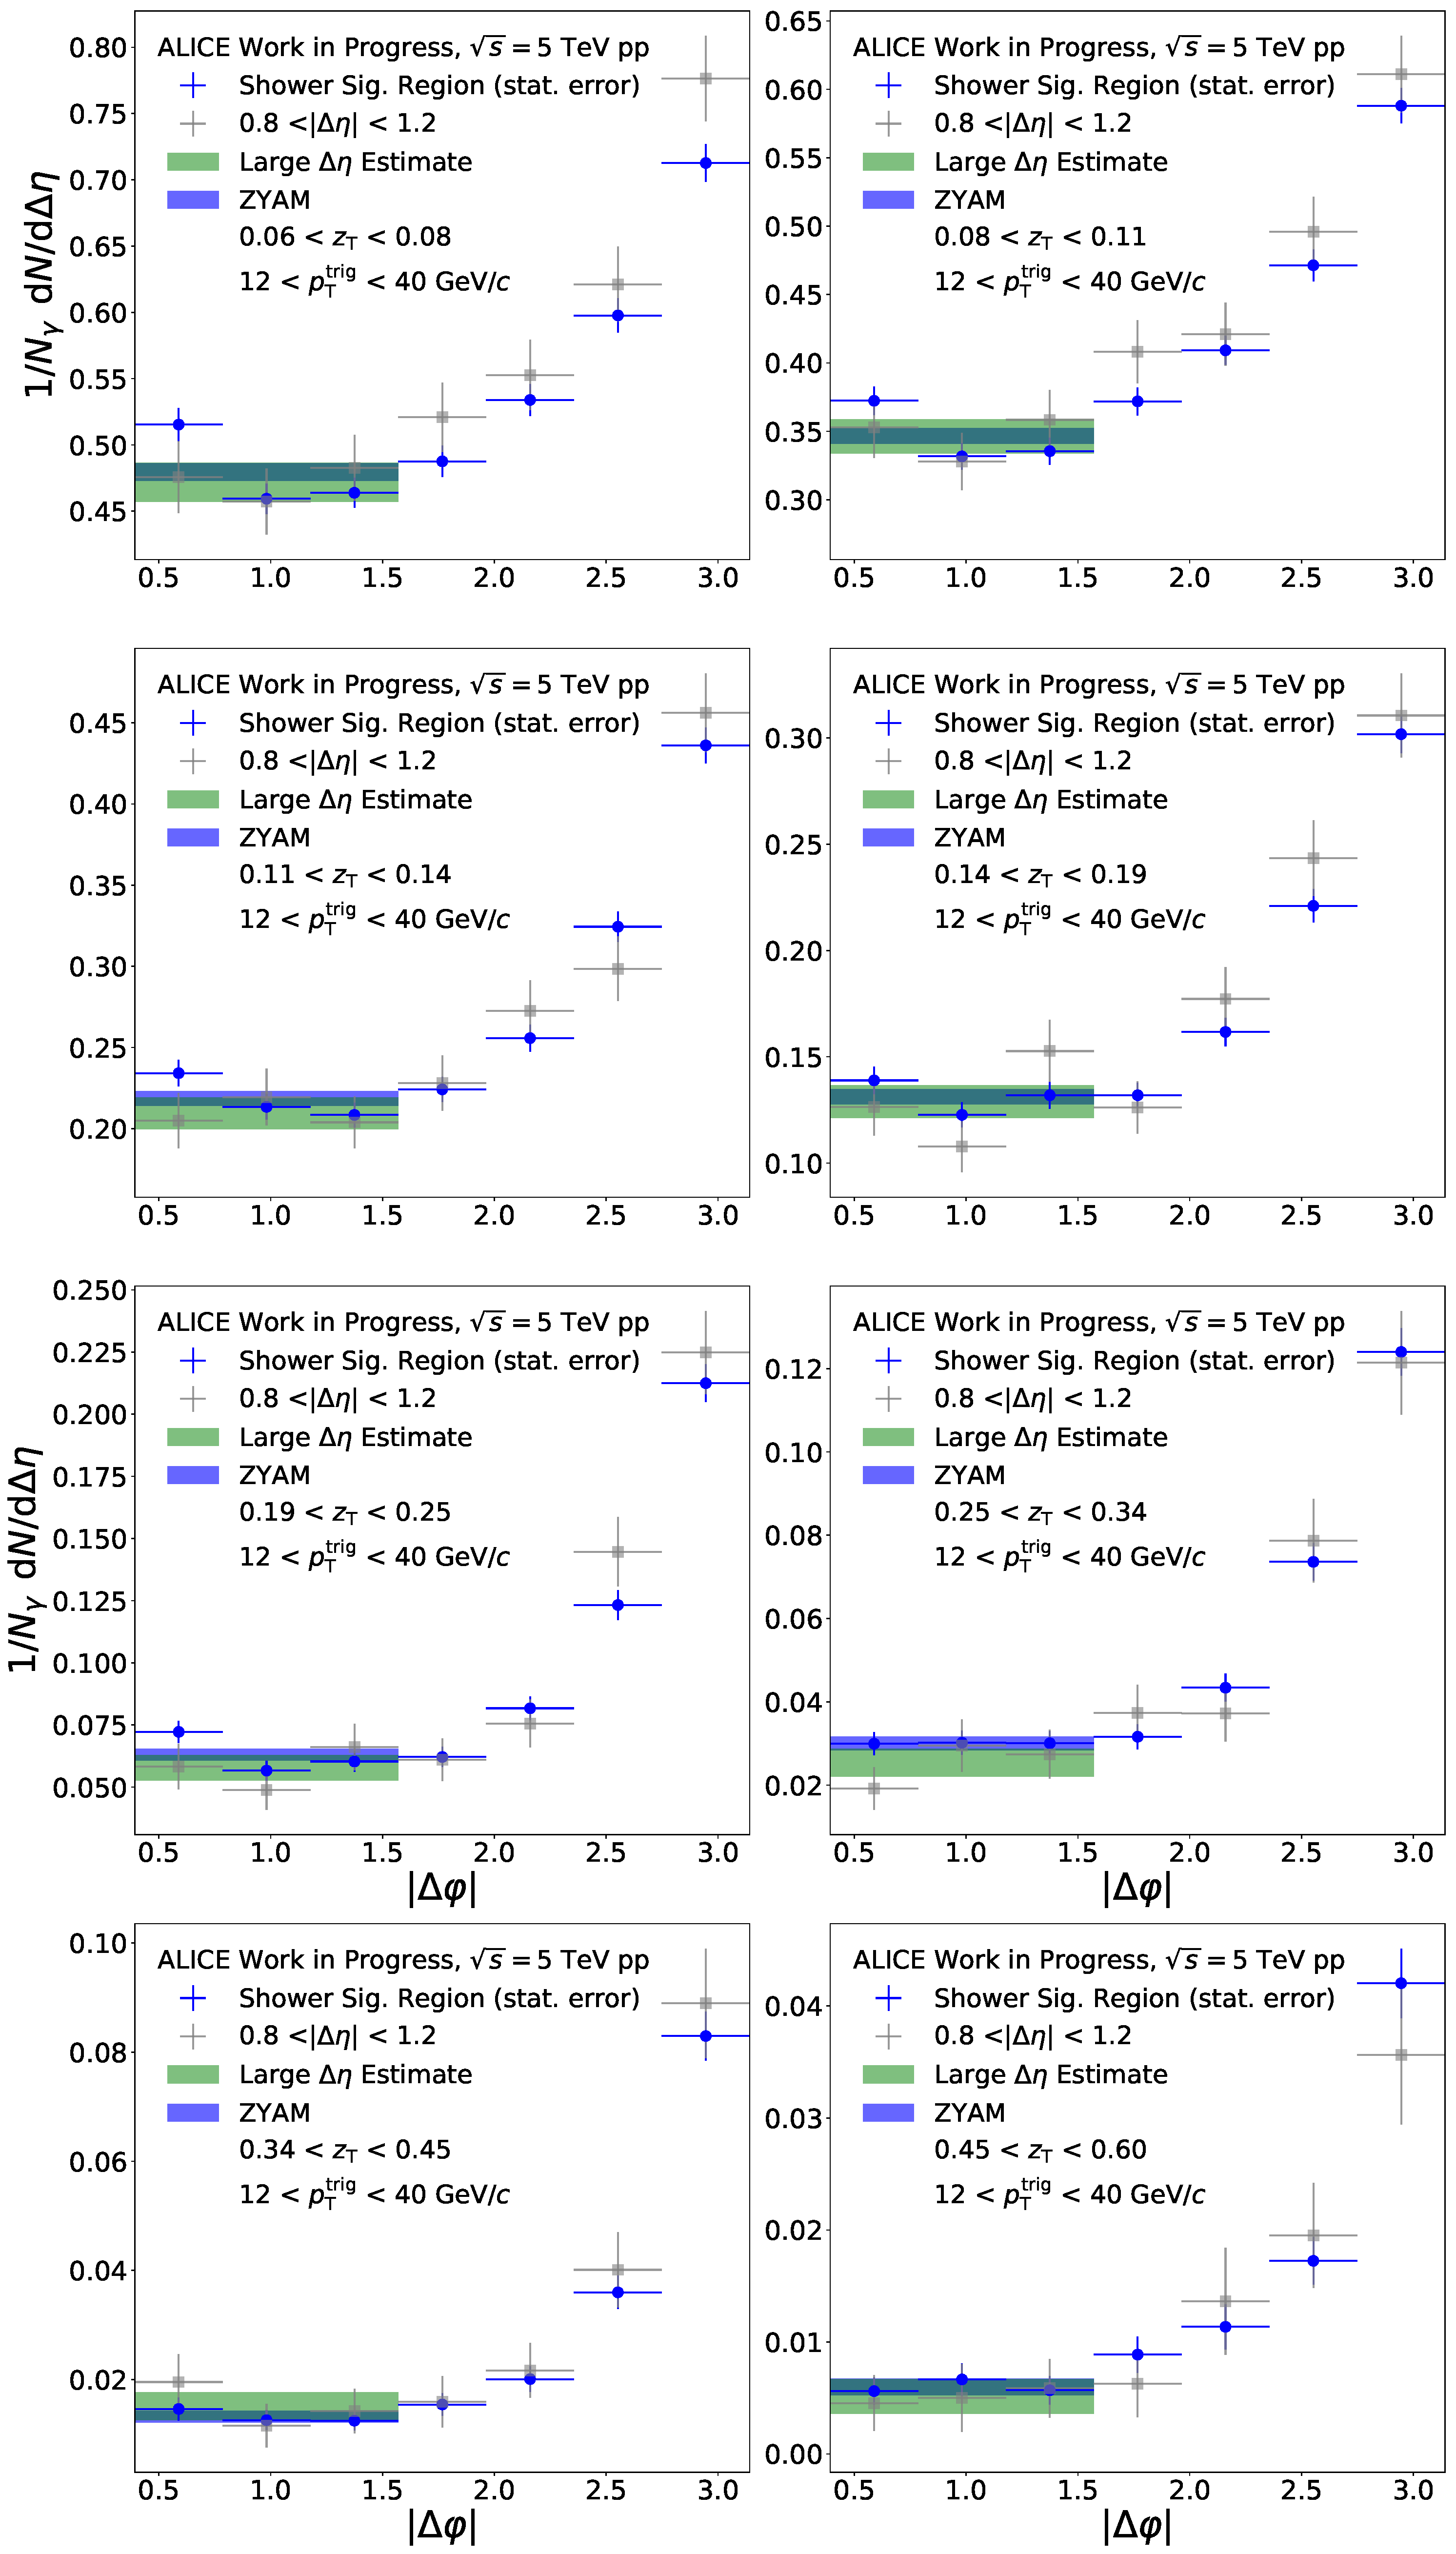
\includegraphics[width=0.8\textwidth]{G-H_New/UE_Plot_pp_pT_0__zT_7.pdf}
%\caption{$\Delta\varphi$ projections of the isolated $\gamma$-hadron correlations in pp collisions with ZYAM (blue) and large $\Delta\eta$ (green) estimates to the uncorrelated background. The empty boxes represent the full $\Delta\varphi$ projection from the large $\Delta\eta$ region.}
%\label{pp_Uncorr}
%\end{figure}

%\begin{figure}[h]
%\center
%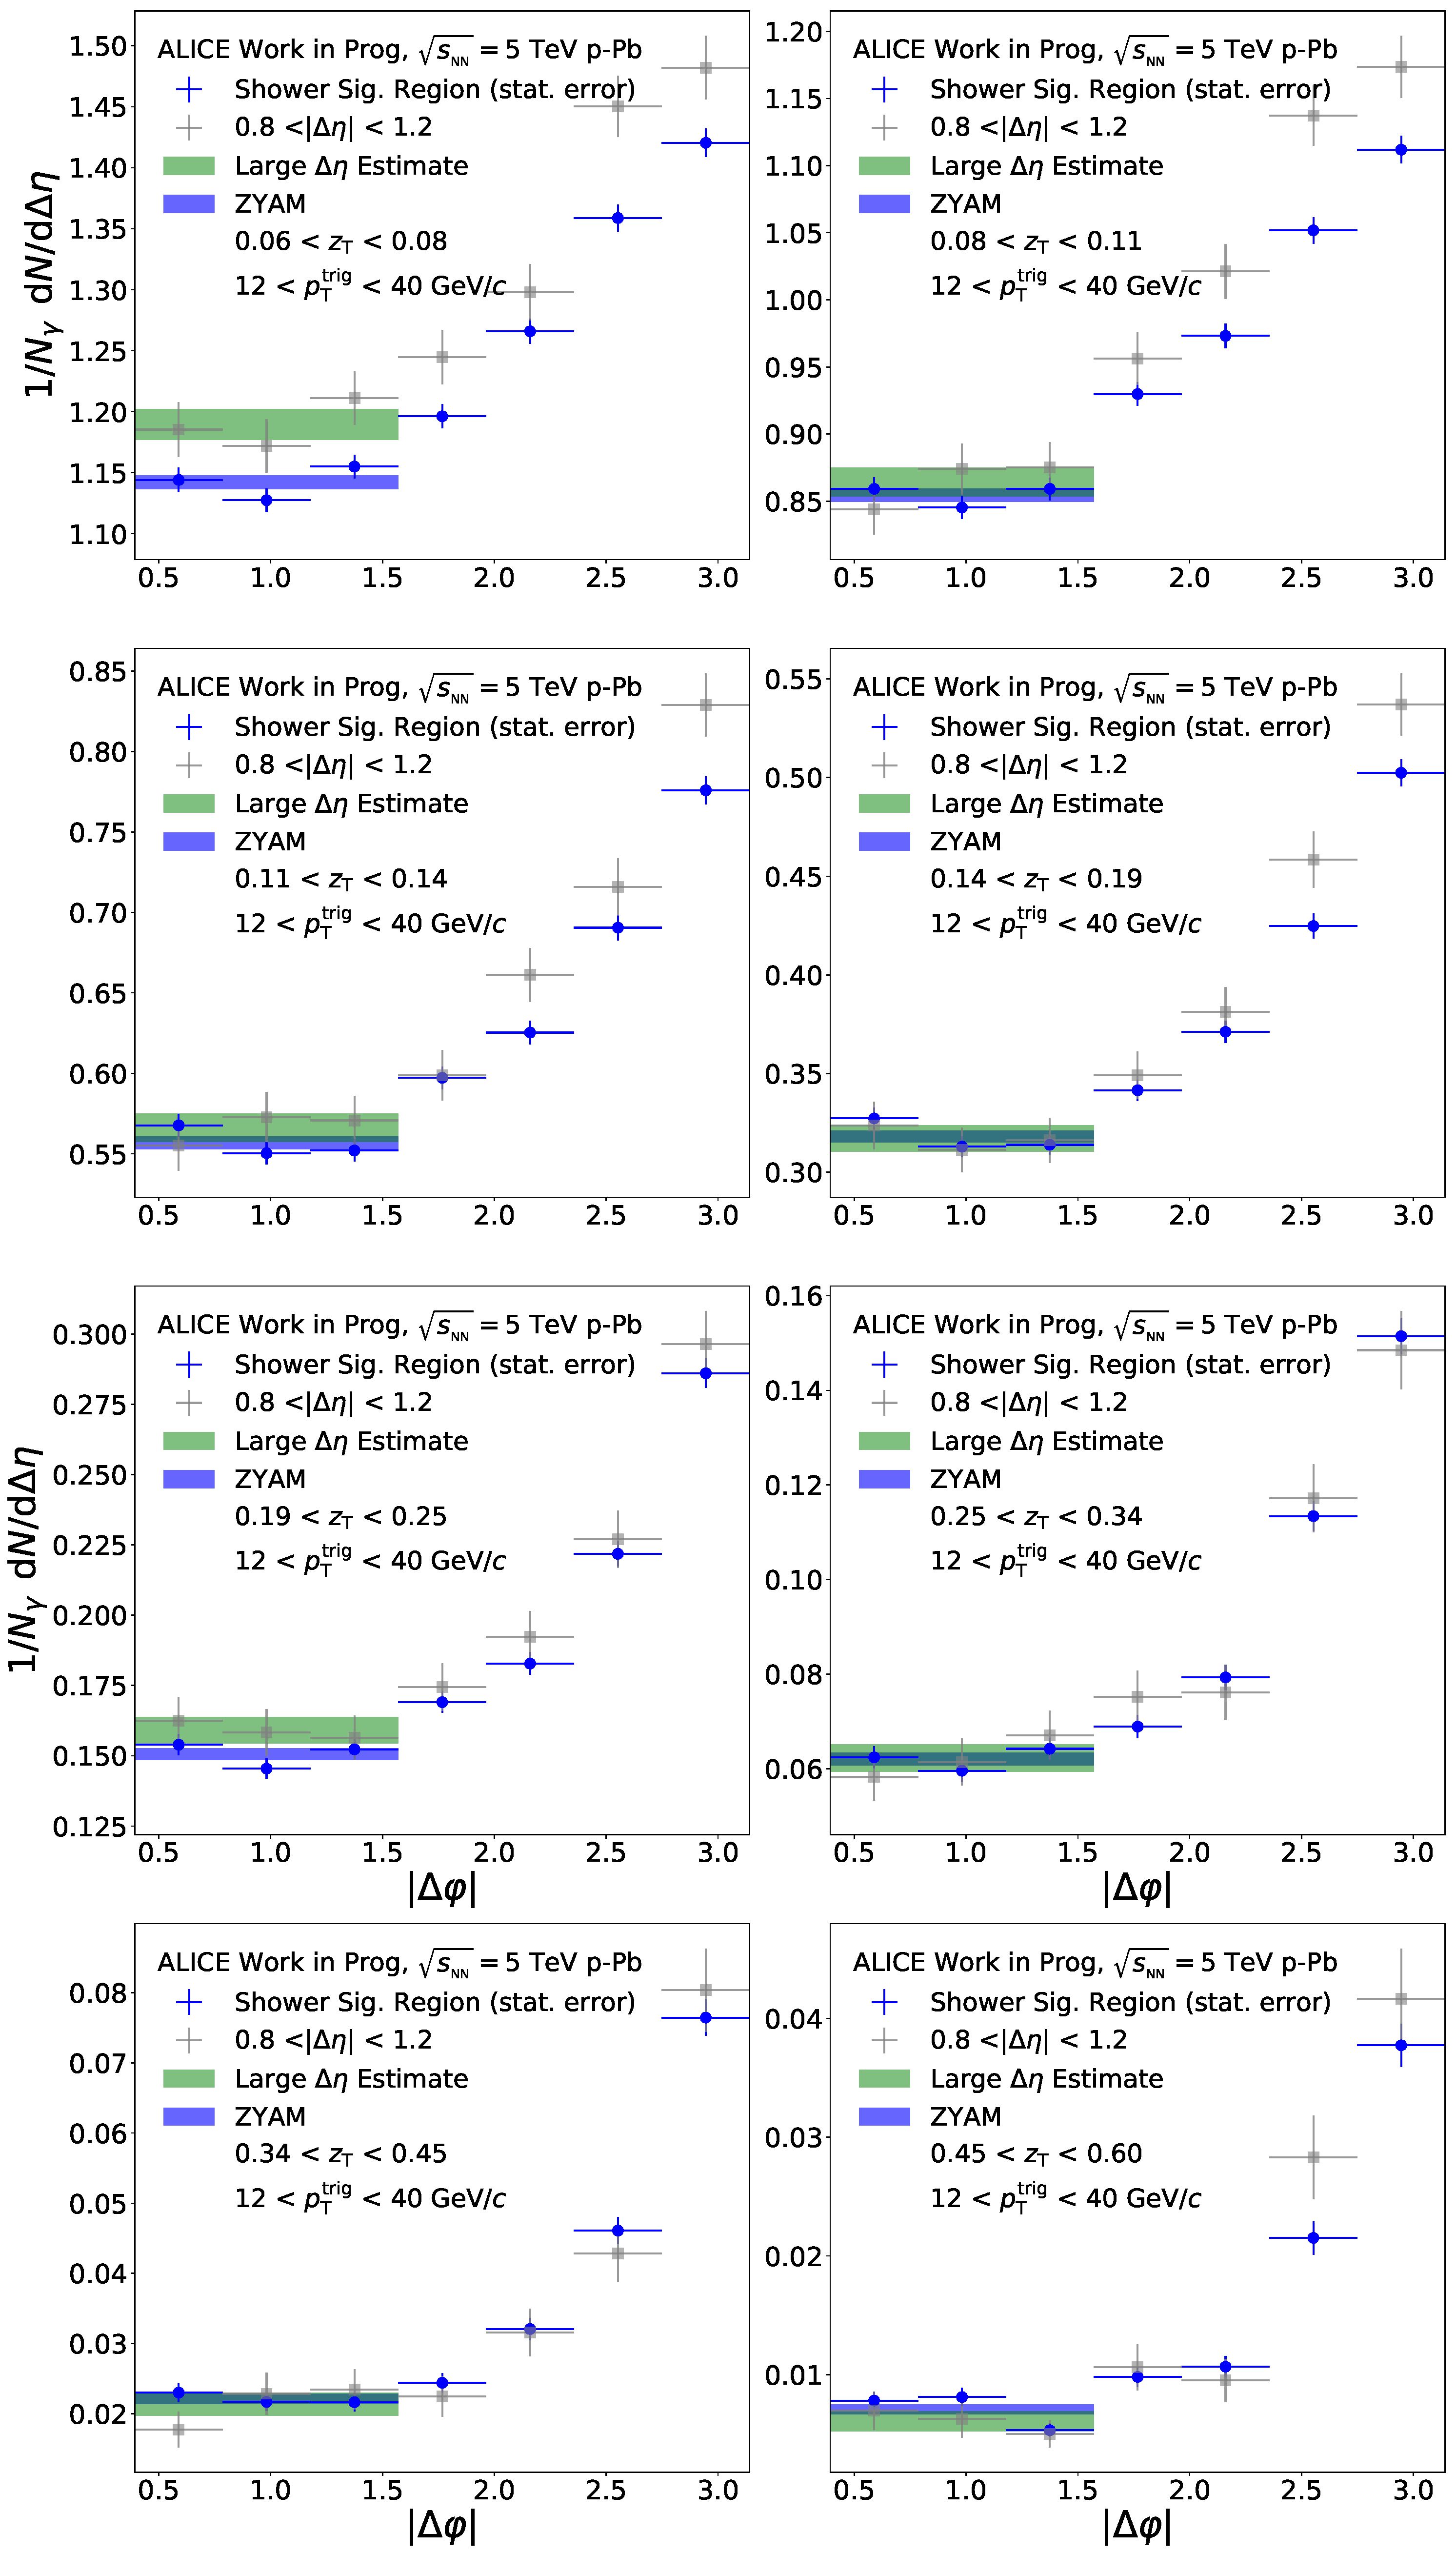
\includegraphics[width=0.8\textwidth]{G-H_New/UE_Plot_p-Pb_pT_0__zT_7.pdf}
%\caption{$\Delta\varphi$ projections of the isolated $\gamma$-hadron correlations in p--Pb collisions with ZYAM (blue) and large $\Delta\eta$ (green) estimates to the uncorrelated background. The empty boxes represent the full $\Delta\varphi$ projection from the large $\Delta\eta$ region. }
%\label{LE_ZYAM}
%\end{figure}

%\subsection{Comment on Order of Subtraction}
%Previous iterations of our analysis used the weighted average purity corresponding to our \lambdasquare cuts shown in Table \ref{tab:shape_table}, albeit for a smaller \pt~range. This gave us the flexibility to subtract the pedestal in both the shower signal and shower background separately, and then scale the two regions according to \ref{eq:FinalSubtraction}. This is shown in figures \ref{fig:Reverse_Sub_UE} and \ref{tab:BigSummaryGammaJet}

%\begin{figure}
%\label{fig:Reverse_Sub_UE}
%\centering
%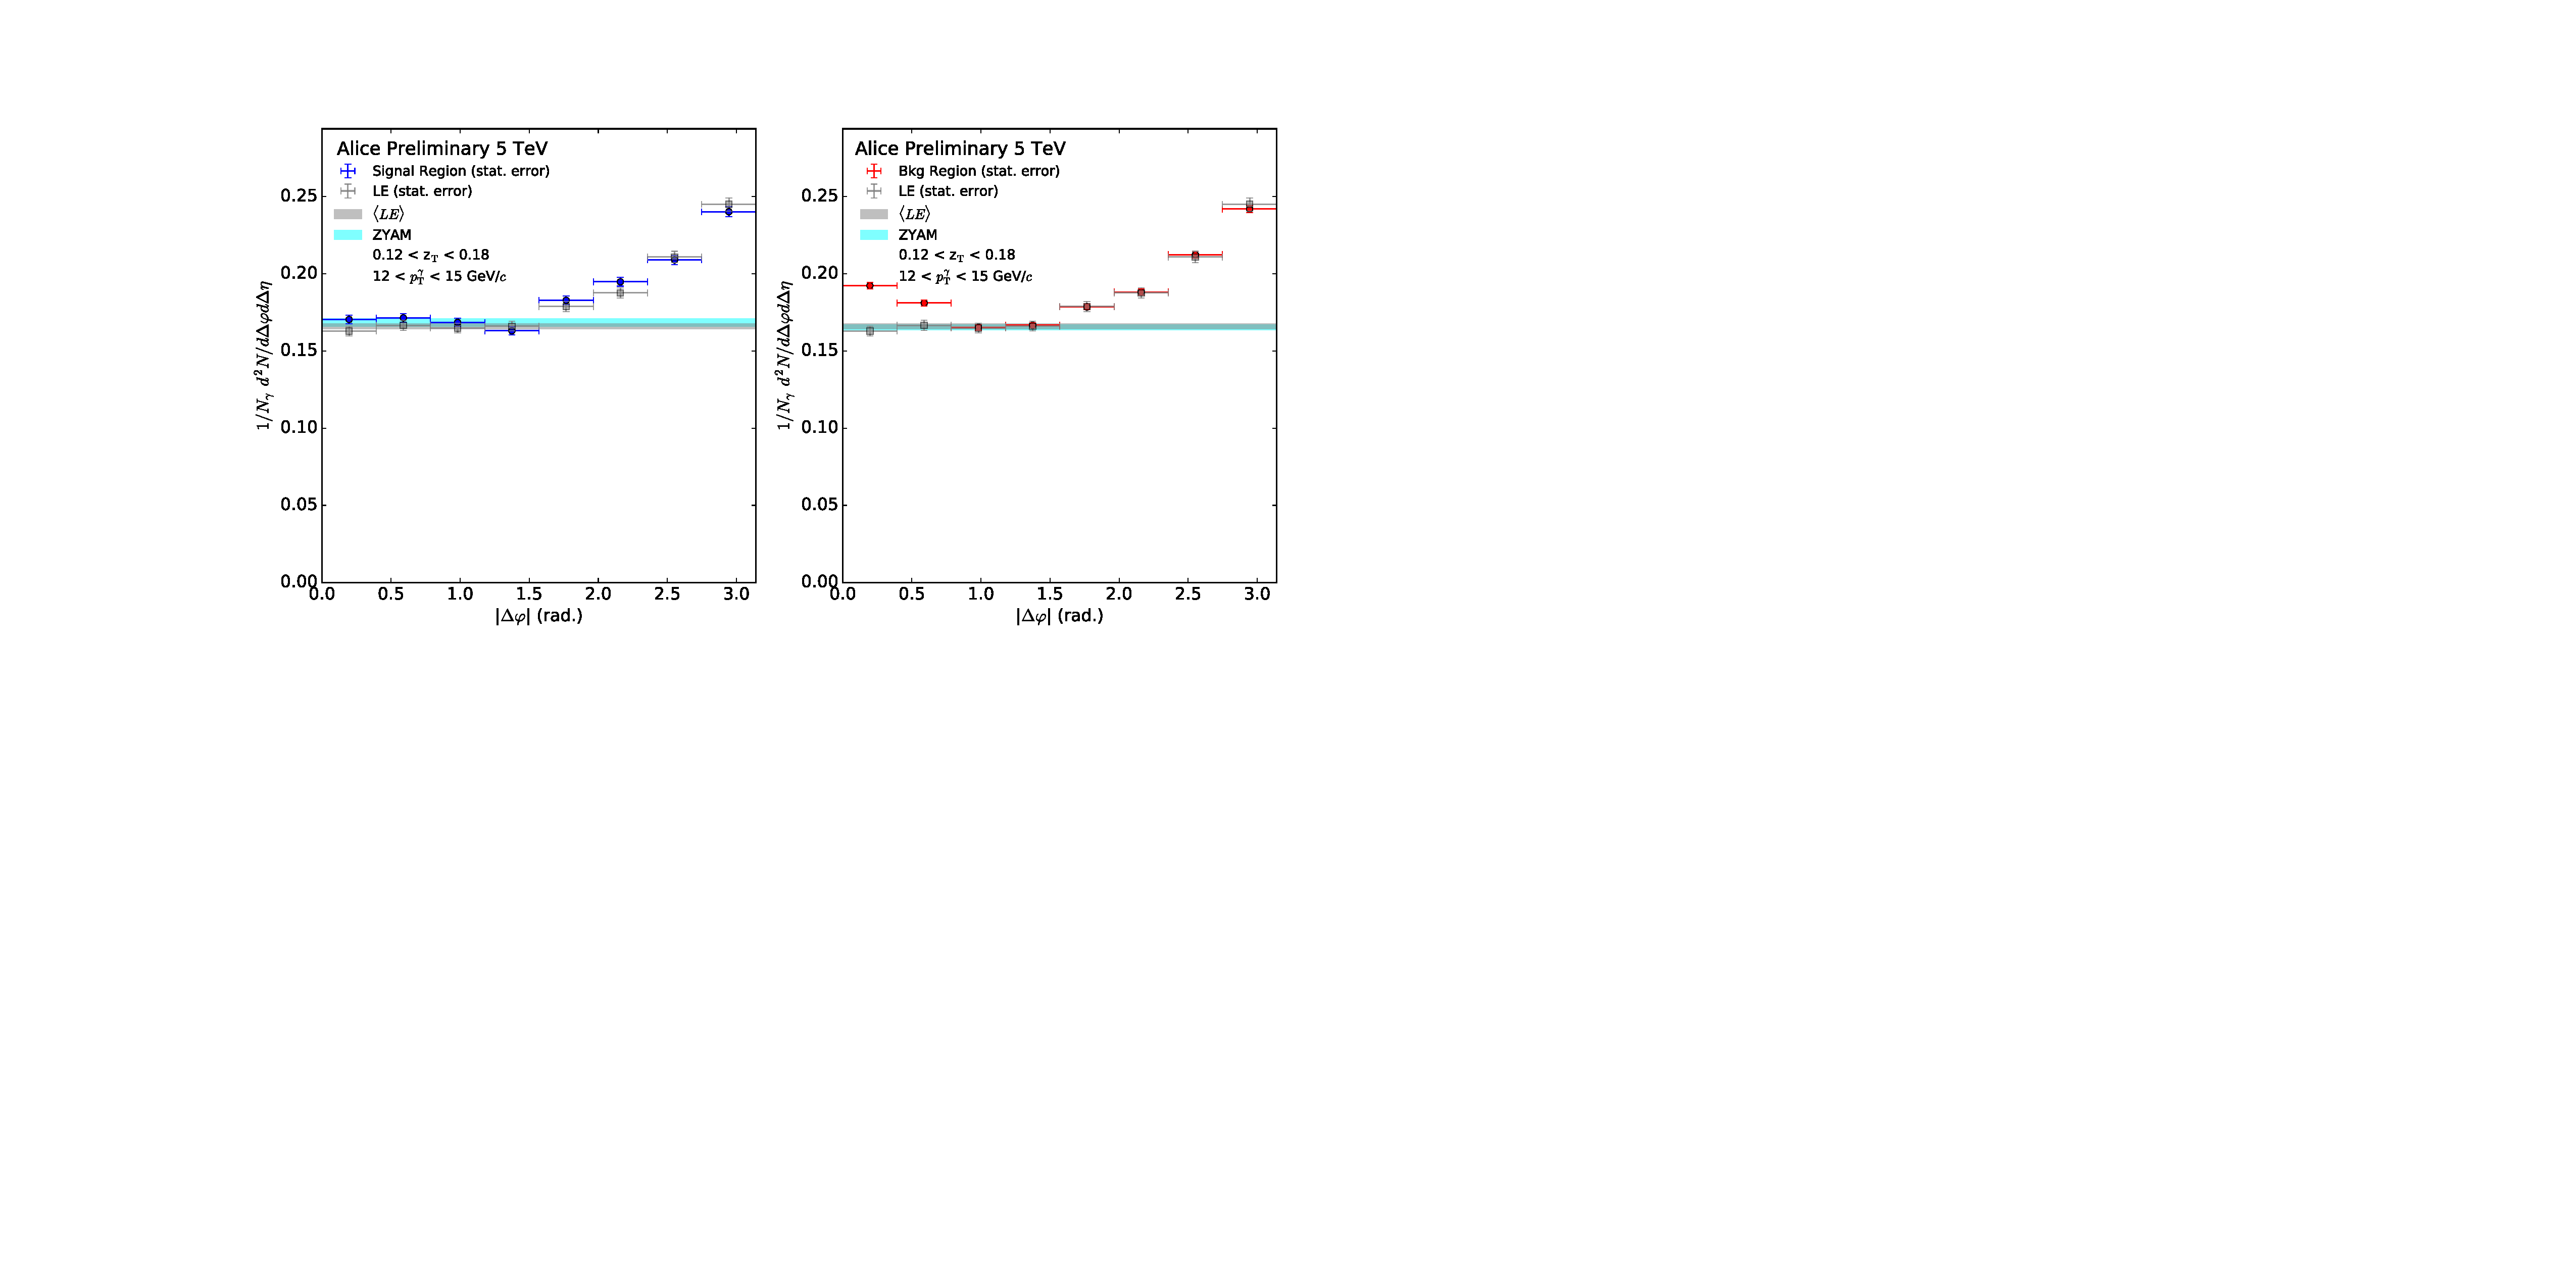
\includegraphics[width=0.5\textwidth]{G-H_New/Reverse_Subtraction_UE_Low_zT}
%\end{figure}

%\begin{figure}
%\label{fig:Reverse_Sub_UE}
%\centering
%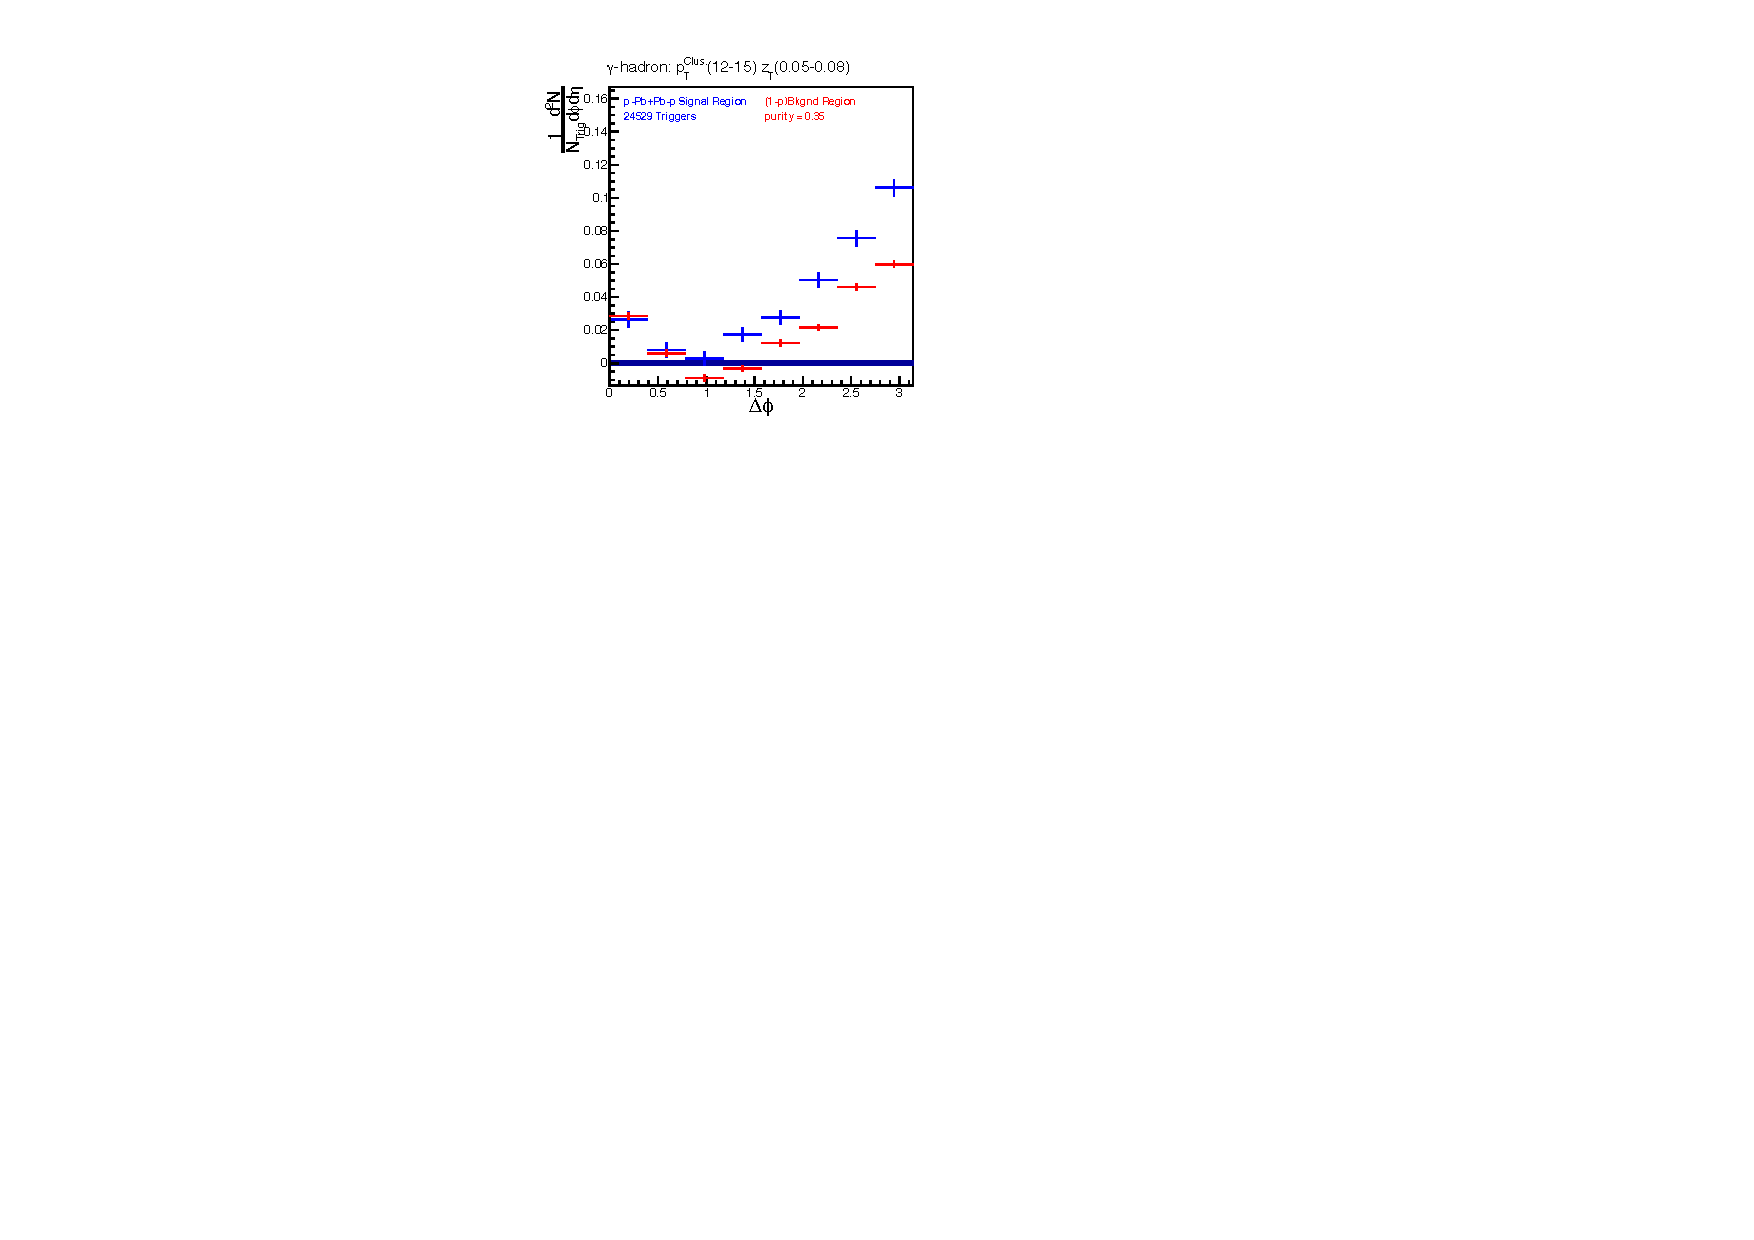
\includegraphics[width=0.5\textwidth]{G-H_New/Reverse_Subtraction_Ov_Low_zT}
%\end{figure}

